%%%%%%%%%%%%%%%%%%%%%%%%%%%%%%%%%%%%%%%%%%%%%%%%%%%%%%%%%%%%%%%%%%%%%%%%%%%%%%%%%%%%%%%%%%%%%%%%%%%
%                                                                                                 %
%         MODELO DE TESE/DISSERTAÇÃO - INSTITUTO DE FÍSICA - UNIVERSIDADE FEDERAL DE GOIÁS        %
%                                by carriunix (stardate 1601.01)                                  %
%                                 marcuscarriao at gmail dot com                                  %
%                                                                                                 %
%%%%%%%%%%%%%%%%%%%%%%%%%%%%%%%%%%%%%%%%%%%%%%%%%%%%%%%%%%%%%%%%%%%%%%%%%%%%%%%%%%%%%%%%%%%%%%%%%%%
%                                                                                                 %
%                                      AVISOS (Leia com atenção)                                  %
%                                                                                                 %
% Este é um modelo NÃO OFICIAL para Teses e Dissertações para alunos do IF-UFG. A intenção deste  %
% material é simplificar, padronizar e personalizar esses trabalhos científicos no âmbito da re-  %
% ferida instituição. Antes de começar a usar este modelo tenha em mente:                         %
%     (i) Ele não segue todas as normas da ABNT (apenas as esteticamente aceitáveis).             %
%    (ii) O modelo é composto por 4 arquivos: UFGmodelo.tex, UFGpreambulo.tex, UFGlogo.png e      %
% IFlogo.png (se você não tem algum desses, provavelmente vai ter problemas)                      %
%   (iii) Este modelo não constitui uma "classe", ele usa um arquivo de definições para ser       %
% usado "sobre" a classe "report" (nativo).                                                       %
%    (iv) Uma série de pacotes serão necessários (todos parte do TeXlive), consulte as primei-    %
% ras linhas do arquivo UFGpreambulo.tex para conhecê-los pessoalmente.                           %
%     (v) Este não é um modelo "for dummies": se você fizer coisa errada... vai dar errado!       %
%    (vi) Siga as instruções abaixo usando como referências as linhas do arquivo não modificado.  %
%                                                                                                 %
%                              INSTRUÇÕES (Leia com mais atenção ainda)                           %
%                                                                                                 %
%   l(76): Escolha as opções que achar conveniente ("oneside" e "twoside" estão disponíveis, mas  %
% os elementos do PRÓLOGO serão sempre "oneside"), mas não altere a classe. Sugiro que você con-  %
% tinue usando o tamanho 12pt (ABNT).                                                             %
%   l(77): Verifique a codificação que você está utilizando.                                      %
%   l(78): Seleção da fonte Times, sugerida por ser estéticamente mais agradável. Se você prefe-  %
% rir usar a Arial (ABNT), comente essa linha e descomente a l(79).                               %
%   l(81): Carregamento do preâmbulo. Verifique opções no próprio arquivo.                        %
%   l(83): Por default, esse é um modelo para doutorandos, se você é um mestrando, comente essa   %
% linha e descomente a seguinte l(84).                                                            %
%   l(85): Entre com o título da sua Tese/Dissertação.                                            %
%   l(86): Caso exista um subtítulo, descomente e preencha esta linha.                            %
%   l(87): Seu nome.                                                                              %
%   l(88): Nome do orientador já com a titulação.                                                 %
%   l(89): Cidade.                                                                                %
%   l(90): Ano com quatro dígitos.                                                                %
%   l(91): Data da defesa no formato "01 de janeiro de 0001"                                      %
%   l(92): Escreva a dedicatória (usando "\\" para saltar linha intencionalmente) ou use o coman- %
% do "\input{file}".                                                                              %
%   l(93): Escreva o texto de uma citação, que aparecerá em itálico e entre aspas.                %
%   l(94): Nome do autor da citação, que aparecerá em negrito precedido por dois traços.          %
%   l(95): Use a função "\input{file}" (preferencialmente) ou escreva o texto dos Agradecimentos. %
%   l(96): Use a função "\input{file}" (preferencialmente) ou escreva o texto do Resumo.          %
%   l(97): Use a função "\input{file}" (preferencialmente) ou escreva o texto do Abstract.        %
%   l(98): Use a função "\input{file}" (preferencialmente) ou escreva o texto do Prefácio. Se vo- %
% cê optar por não ter um Prefácio, comente essa linha e também a l(109).                         %
%   l(102): Invocação da estrutura da capa (obrigatória).                                         %
%   l(103): Invocação da estrutura da folha de rosto (obrigatória).                               %
%   l(104): Invocação da estrutura da folha de aprovação (obrigatória apenas na versão final).    %
%   l(105): Invocação da estrutura da dedicatória (opcional, comente se preferir não usar).       %
%   l(106): Invocação da estrutura dos agradecimentos (opcional, comente se preferir não usar).   %
%   l(107): Invocação da estrutura da epígrafe (opcional, comente se preferir não usar).          %
%   l(108): Invocação da estrutura do resumos em português  e inglês (obrigatório). Usa espaça-   %
% mento simples como sugerem as normas da ABNT.                                                   %
%   l(109): Invocação da estrutura do prefácio (opcional, comente se preferir não usar).          %
%   l(110): Invocação da estrutura do sumário (obrigatório).                                      %
%   l(111): Inclua nesta linha outras listas (figuras, tabelas, abreviaturas, simbolos, etc) que  %
% estejam sendo usadas no seu trabalho (elementos opcionais).                                     %
%   l(113): Início da numeração arábica das páginas e dos Elementos Texuais. A partir daqui, es-  %
% colha entre escrever o conteúdo diretamente neste arquivo ou usar a função "\input{file}" para  %
% incluí-lo (preferencialmente).                                                                  %
%   l(135): Informe o nome do arquivo BibTeX (*.bib) de referências.                              %
%   l(136): Informe o estilo de apresentação das referências.                                     %
%   l(137): Se você optar por inserir as referências manualmente (ou copiar o arquivo *.bbl), co- %
% mente l(135) e l(136) e descomente o ambiente "thebibliography" l(137), l(138) e l(139).        %
%   l(140): Início dos Apêndices, identificados com letras. Escreva o conteúdo diretamente neste  %
% arquivo ou usar a função "\input{file}" para incluí-lo.                                         %
%                                                                                                 %
%                                       That's all, folks!                                        %
%                                   May the Force be with you.                                    %
%%%%%%%%%%%%%%%%%%%%%%%%%%%%%%%%%%%%%%%%%%%%%%%%%%%%%%%%%%%%%%%%%%%%%%%%%%%%%%%%%%%%%%%%%%%%%%%%%%%


\documentclass[twoside,openright,12pt,a4paper]{report}
\usepackage[utf8]{inputenc}
\usepackage{times}

%%%%%%%%%%%%%%%%%%%%%%%%%%%%%%%%%%%%%%% CARREGANDO PREÂMBULO %%%%%%%%%%%%%%%%%%%%%%%%%%%%%%%%%%%%%%
\usepackage[left=3cm, right=2cm, top=3cm, bottom=2cm]{geometry}
\usepackage[english]{babel}
\usepackage{setspace}
\usepackage{amsmath}
\usepackage{amssymb}
\usepackage{amsthm}
\usepackage{acronym}
\usepackage{graphicx}
\usepackage{subfigure}
\usepackage{icomma} 
\usepackage{verbatim}
\usepackage{enumitem}
\usepackage{arydshln}
\usepackage{xspace}
\usepackage{ragged2e}
\usepackage{float}
\usepackage{titlesec}
\usepackage{emptypage}
\usepackage{indentfirst}
\usepackage{xcolor}
\usepackage{lipsum}
\usepackage{fix-cm}
\usepackage{tikz}
\usepackage{fancyhdr}
\usepackage[mathlines]{lineno}
\usepackage{cite}
\usepackage{hyperref}

\hypersetup{
    colorlinks=true,
    linkcolor=black,
    filecolor=magenta,      
    urlcolor=blue,
    citecolor=black
}
\urlstyle{same}

\usepackage{etoolbox}
\let\bbordermatrix\bordermatrix
\patchcmd{\bbordermatrix}{8.75}{4.75}{}{}
\patchcmd{\bbordermatrix}{\left(}{\left[}{}{}
\patchcmd{\bbordermatrix}{\right)}{\right]}{}{}

\usepackage{caption}
\DeclareCaptionLabelSeparator{bar}{\raisebox{0.75pt}{\space$\pmb{\vert}$\space}}
\captionsetup{labelfont=bf,labelsep=bar,font=small, width=0.95\textwidth}

\usepackage{booktabs}
\usepackage{multirow}


\renewcommand{\arraystretch}{1.2}
\newlength{\Oldarrayrulewidth}
\newcommand{\Cline}[2]{%
  \noalign{\global\setlength{\Oldarrayrulewidth}{\arrayrulewidth}}%
  \noalign{\global\setlength{\arrayrulewidth}{#1}}\cline{#2}%
  \noalign{\global\setlength{\arrayrulewidth}{\Oldarrayrulewidth}}
}





\fancypagestyle{plain}{
\fancyhf{}
\fancyfoot[C]{\bfseries \thepage}
\renewcommand{\headrulewidth}{0pt}
\renewcommand{\footrulewidth}{0pt}}

\fancypagestyle{myheadings}{
\fancyhf{}
\fancyhead[LE,RO]{\bfseries \thepage}
\fancyhead[LE,RO]{\bfseries \thepage}
\renewcommand{\headrulewidth}{0.4pt}
\renewcommand{\footrulewidth}{0pt}}

\onehalfspacing
\newcommand{\verso}{\newpage\null\thispagestyle{empty}\newpage}
\definecolor{ufgblue}{RGB}{240,255,240}


\newif\ifisappendix
\isappendixfalse

\titleformat{\chapter}[display]
  {\bfseries\huge}
  {\vspace*{-3cm}\filright{\begin{tikzpicture}
 	\ifisappendix
      % \draw[xshift=1.4cm, yshift=1cm,fill,color=ufgblue] (30:1cm) -- (90:1cm) -- (150:1cm) -- (210:1cm) -- (270:1cm) -- (330:1cm) -- (30:1cm);
% Para imprimir o \chaptername antes no número/letra do capítulo/anexo, descomente a linha abaixo:
       \draw[color=black] (-2.2cm,0.8cm) node { \fontsize{31.5}{41.5}\selectfont \chaptername };
       \draw[color=black] (1.4cm,1.cm) node { \fontsize{41.5}{51.5}\selectfont \thechapter };
    \else
       %\draw[xshift=1.cm, yshift=1cm,fill,color=ufgblue] (30:1cm) -- (90:1cm) -- (150:1cm) -- (210:1cm) -- (270:1cm) -- (330:1cm) -- (30:1cm);
% Para imprimir o \chaptername antes no número/letra do capítulo/anexo, descomente a linha abaixo:
       %\draw[color=black] (-2.2cm,0.8cm) node { \fontsize{31.5}{41.5}\selectfont \chaptername };
       \draw[color=black] (1.cm,1.cm) node { \fontsize{41.5}{51.5}\selectfont \thechapter };
	\fi
    \end{tikzpicture} } }
  {2cm}
  {\filleft}
  [\vspace{-0.6cm}\rule{\textwidth}{1.6pt}\\ \vspace*{-1.05cm}\rule{\textwidth}{0.4pt}]

\makeatletter


\newcommand{\course}{Department of Physics\xspace}
\newcommand{\college}{College of Arts and Sciences\xspace}
\newcommand{\university}{Syracuse University\xspace}
\newtoks\tipo
\newcommand{\type}{\the\tipo\xspace}
\newtoks\grau
\newtoks\gt
\newcommand{\degree}{\the\grau\xspace}
\newtoks\titulo
\renewcommand{\title}{\the\titulo\xspace}
\newcommand{\subtitle}{\the\subtitulo\xspace}
\newtoks\autor
\renewcommand{\author}{\the\autor\xspace}
\newtoks\cidade
\newcommand{\local}{\the\cidade\xspace}
\newtoks\ano
\renewcommand{\year}{\the\ano\xspace}
\newtoks\data
\renewcommand{\date}{\the\data\xspace}
\newtoks\orientador
\newcommand{\advisor}{\the\orientador\xspace}
\newtoks\coorientador
\newcommand{\coadvisor}{\the\coorientador\xspace}
\newtoks\dedicatoria
\newtoks\epigrafe
\newtoks\autordaepigrafe
\newtoks\agradecimento
\newtoks\resumo
\newtoks\abstract
\newtoks\prefacio


\pagestyle{plain}

\newcommand{\capa}{\begin{titlepage}
  \centering
  \vspace*{2cm}
  \rule{12cm}{1.6pt}\\ \vspace*{-0.55cm}
  \rule{12cm}{0.4pt}\\
  \begin{minipage}[t][5.5cm][t]{11.5cm}
  \vspace*{\fill}
  \centering
  \baselineskip=40pt
  {\Huge \bf \title}\\[\baselineskip]
  \ifx\subtitulo\undefined
  \vspace{0.1cm}
  \else
  {\Large \itshape \subtitle}\\[0.2\baselineskip]
  \fi
  \vspace*{\fill}
  \end{minipage}\\
  \rule{12cm}{0.4pt}\\ \vspace*{-0.5cm}
  \rule{12cm}{1.6pt}\\[\baselineskip]
  \vspace{0.5cm}
  
\includegraphics[width=3.8cm]{Logos/SYRACUSE_heritage_ORANGE_RGB.png}\\
  \vspace{1cm}
  {\Large \author}\par
  \vspace{1cm}
  {\scshape \course}\\
  {\scshape \college}\\
  {\scshape \university}\\
  \vfill
  {\small \type presented as a partial fulfillment of the requirements for the degree of}\\[\baselineskip]
  {\small\itshape \degree in Physics}\\[\baselineskip]
  {\large\scshape \local}\\[\baselineskip]
  {\small\scshape \year}\par
  \vspace*{0.05\textheight}
  \end{titlepage}%
}

\newcommand{\paginaTECA}{\begingroup
  \thispagestyle{empty}
  \centering
  \vspace*{\fill}
  {\Large Página dedicada ao Termo de Ciência e Autorização (TECA)}
  \vspace*{\fill}
  \endgroup
  \newpage
}


\newcommand{\folhaderosto}{\begingroup
  \thispagestyle{empty}
  \centering
  \begin{tabular}{p{2cm} p{10cm} p{2cm}}
  \centering 
\includegraphics[width=2cm]{Logos/SYRACUSE_heritage_ORANGE_RGB.png} & \centering \vspace{-1.65cm} \scshape \university \par \college \par \course& \centering \includegraphics[width=2.5cm]{}\\
  \end{tabular}\\
  \vspace*{2cm}
  \begin{minipage}[t][6cm][c]{12cm}
  \centering
  {\Large \author \\}
  \vspace{1cm}
  \baselineskip=30pt
  {\Huge \title}
  \ifx\subtitulo\undefined
  \vspace{0.1cm}
  \else
  {\Large \itshape \subtitle}\\[0.2\baselineskip]
  \fi
  \end{minipage}\\[\baselineskip]
  \hspace{7cm}
  \begin{minipage}[t][5cm][t]{7cm}
   %\type submitted to the \course of the \college of the \university, in partial fulfillment for the degree of \degree in Physics, under the advising of \advisor, with the co-advising of \coadvisor.
   \type submitted to the \course of the \college of the \university, in partial fulfillment for the degree of \degree in Physics, under the advising of \advisor.

  \end{minipage}\\
  \vfill
  {\large\scshape \local}\\[\baselineskip]
  {\small\scshape \year}\par
  \vspace*{0.05\textheight}
  \endgroup
  \newpage
}


\newcommand{\paginaFichaCatalografica}{\begingroup
  \thispagestyle{empty}
  \centering
  \vspace*{\fill}
  {\Large Página dedicada à FICHA CATALOGRÁFICA.}
  \vspace*{\fill}
  \endgroup
  \newpage
}



\newcommand{\folhadeaprovacao}{\begingroup
  \thispagestyle{empty}
  \centering
  \vspace*{\fill}
  {\Large Substitua essa folha pela FOLHA DE APROVAÇÃO ou ATA DA DEFESA.}
  \vspace*{\fill}
  \endgroup
  \verso
}




\newcommand{\adedicatoria}{\begingroup
  \thispagestyle{empty}
  \centering
  \vspace*{\fill}
  \hspace{7cm}
  \begin{minipage}[t][5cm][t]{8.2cm}
  {\itshape \vfill \hfill  \the\dedicatoria} 
  \end{minipage}\\[\baselineskip]
  \vspace*{3cm}
  \endgroup
  \verso
}

% small epigraph
\newcommand{\acitacao}{\begingroup
  \thispagestyle{empty}
  \vspace*{\fill}
  \hspace{7cm}
  \begin{minipage}[t][5cm][t]{8.2cm}
  \begin{raggedright}
    \it ``\the\epigrafe"
  \end{raggedright}  
  \begin{flushright}
	\bf \the\autordaepigrafe
  \end{flushright}
  \end{minipage}\\[\baselineskip]
  \endgroup
}

%
%% full line epigraph
%\newcommand{\acitacao}{\begingroup
%  \thispagestyle{empty}
%  \vspace*{\fill}
%  \begin{raggedright}
%    \it ``\the\epigrafe"
%  \end{raggedright}  
%  \begin{flushright}
%	\bf -- \the\autordaepigrafe
%  \end{flushright}
%  \endgroup
%}


\newcommand{\notaagradecimento}{\chapter*{Acknowledgements}
  \addcontentsline{toc}{chapter}{\protect\numberline{}Acknowledgements}
  \pagenumbering{roman}
  \setcounter{page}{9}
  \the\agradecimento
  \vspace*{\fill}
  \verso
}

\newcommand{\resumos}{\chapter*{Abstract}
  \addcontentsline{toc}{chapter}{\protect\numberline{}Abstract}
  \singlespacing
  \the\abstract
  \vspace*{\fill}
  \onehalfspacing
  \chapter*{Resumo}
  \addcontentsline{toc}{chapter}{\protect\numberline{}Resumo}
  \singlespacing 
  \the\resumo
  \vspace*{\fill}
  \onehalfspacing
  \verso
}

\newcommand{\apresentacao}{\chapter*{Preface}
  \addcontentsline{toc}{chapter}{\protect\numberline{}Preface}
  \singlespacing 
  \the\prefacio
  \vspace*{\fill}
  \onehalfspacing
}

\newcommand{\inicio}{
  \newpage
  \pagestyle{myheadings}
  \pagenumbering{arabic}
  \setcounter{page}{1}
  
  \renewcommand\chapter{\if@openright\cleardoublepage\else\clearpage\fi
                    \thispagestyle{empty}%
                    \global\@topnum\z@
                    \@afterindentfalse
                    \secdef\@chapter\@schapter}
                    
}


%%%%%%%%%%%%%%%%%%%%%%%%%%%%%%%%%%% INFORMAÇÕES GERAIS DA TESE %%%%%%%%%%%%%%%%%%%%%%%%%%%%%%%%%%%%
% Tipo
\tipo{Dissertation} \grau{Doctor of Philosophy}
%\tipo{Thesis} \grau{Master}


\titulo{~\\Search for NuMI $\mu$DAR Electron Neutrinos in MicroBooNE”}
%\newtoks\subtitulo \subtitulo{Morte e Obra} 
\autor{Ohana Benevides Rodrigues}
\orientador{Professor Mitchell Soderberg}
\coorientador{}
\cidade{Syracuse - NY}
\ano{2022}
\data{September 02}


\dedicatoria{To my parents, Andrea de Fátima Benevides and Luis Claudio Rocha Rodrigues.}


\epigrafe{Knowledge emerges only through invention and reinvention, through the restless, impatient, continuing, hopeful inquiry human beings pursue in the world, with the world, and with each other.}
\autordaepigrafe{Paulo Freire}

\agradecimento{

The acknowledgements.

}


\abstract{

\lipsum[1-3]

}

%\prefacio{\lipsum[1-3]}

\begin{document}

%%%%%%%%%%%%%%%%%%%%%%%%%%%%%%%%%%%%%%%%%% PRÓLOGO %%%%%%%%%%%%%%%%%%%%%%%%%%%%%%%%%%%%%%%%%%%%%%%%
\capa
%\paginaTECA
%\folhaderosto
%\paginaFichaCatalografica
\folhadeaprovacao
\adedicatoria
\notaagradecimento
\acitacao
%\resumos
%\apresentacao
\tableofcontents
\listoffigures 
\listoftables
\linenumbers

%%%%%%%%%%%%%%%%%%%%%%%%%%%%%%%%%%% CORPO DA TESE/DISSERTAÇÃO %%%%%%%%%%%%%%%%%%%%%%%%%%%%%%%%%%%%%
\inicio

\chapter{Introduction}
\section{Neutrino Physics Historical Overview}
\label{Chapter:1}

\subsection{The Beta Decay Problem}

Radioactivity was discovered in 1896 by Henri Becquerel. A few years later, in 1899, Ernest Rutherford classified radioactivity emissions into two types: $\alpha$ and $\beta$. In the occasion, Rutherford conjectured that the beta decay was a two-body decay. In such case, the decay would be characterized by a nucleus A becoming a lighter nucleus B, with the emission of an electron, like the following:
%
\begin{equation}
	A \longrightarrow B + e^- .
\end{equation}
%
Consequently, the energies of the outgoing particles would be kinematically determined. 
Using conservation of energy and momentum, it is straightforward to conclude that this energy should be:
%
\begin{equation}
	E = \frac{m_A^2 - m_B^2 + m_e^2}{2m_A} c^2.
	\label{electron_max_energy} 
\end{equation}
%
Experiments conducted by Lise Meitner and Otto Han in 1911 demonstrated that the energy spectrum of the electron coming out of the $\beta$ decay was, in fact, not well-defined, as expected if it was two-body decay. The electron energy spectrum was continuous, having the maximum energy defined by the equation \ref{electron_max_energy} (see figure \ref{figure_the_beta_decay_spectrum_of_tritium}) \cite{griffiths}.
%
\begin{figure}[h!]
	\begin{center}
		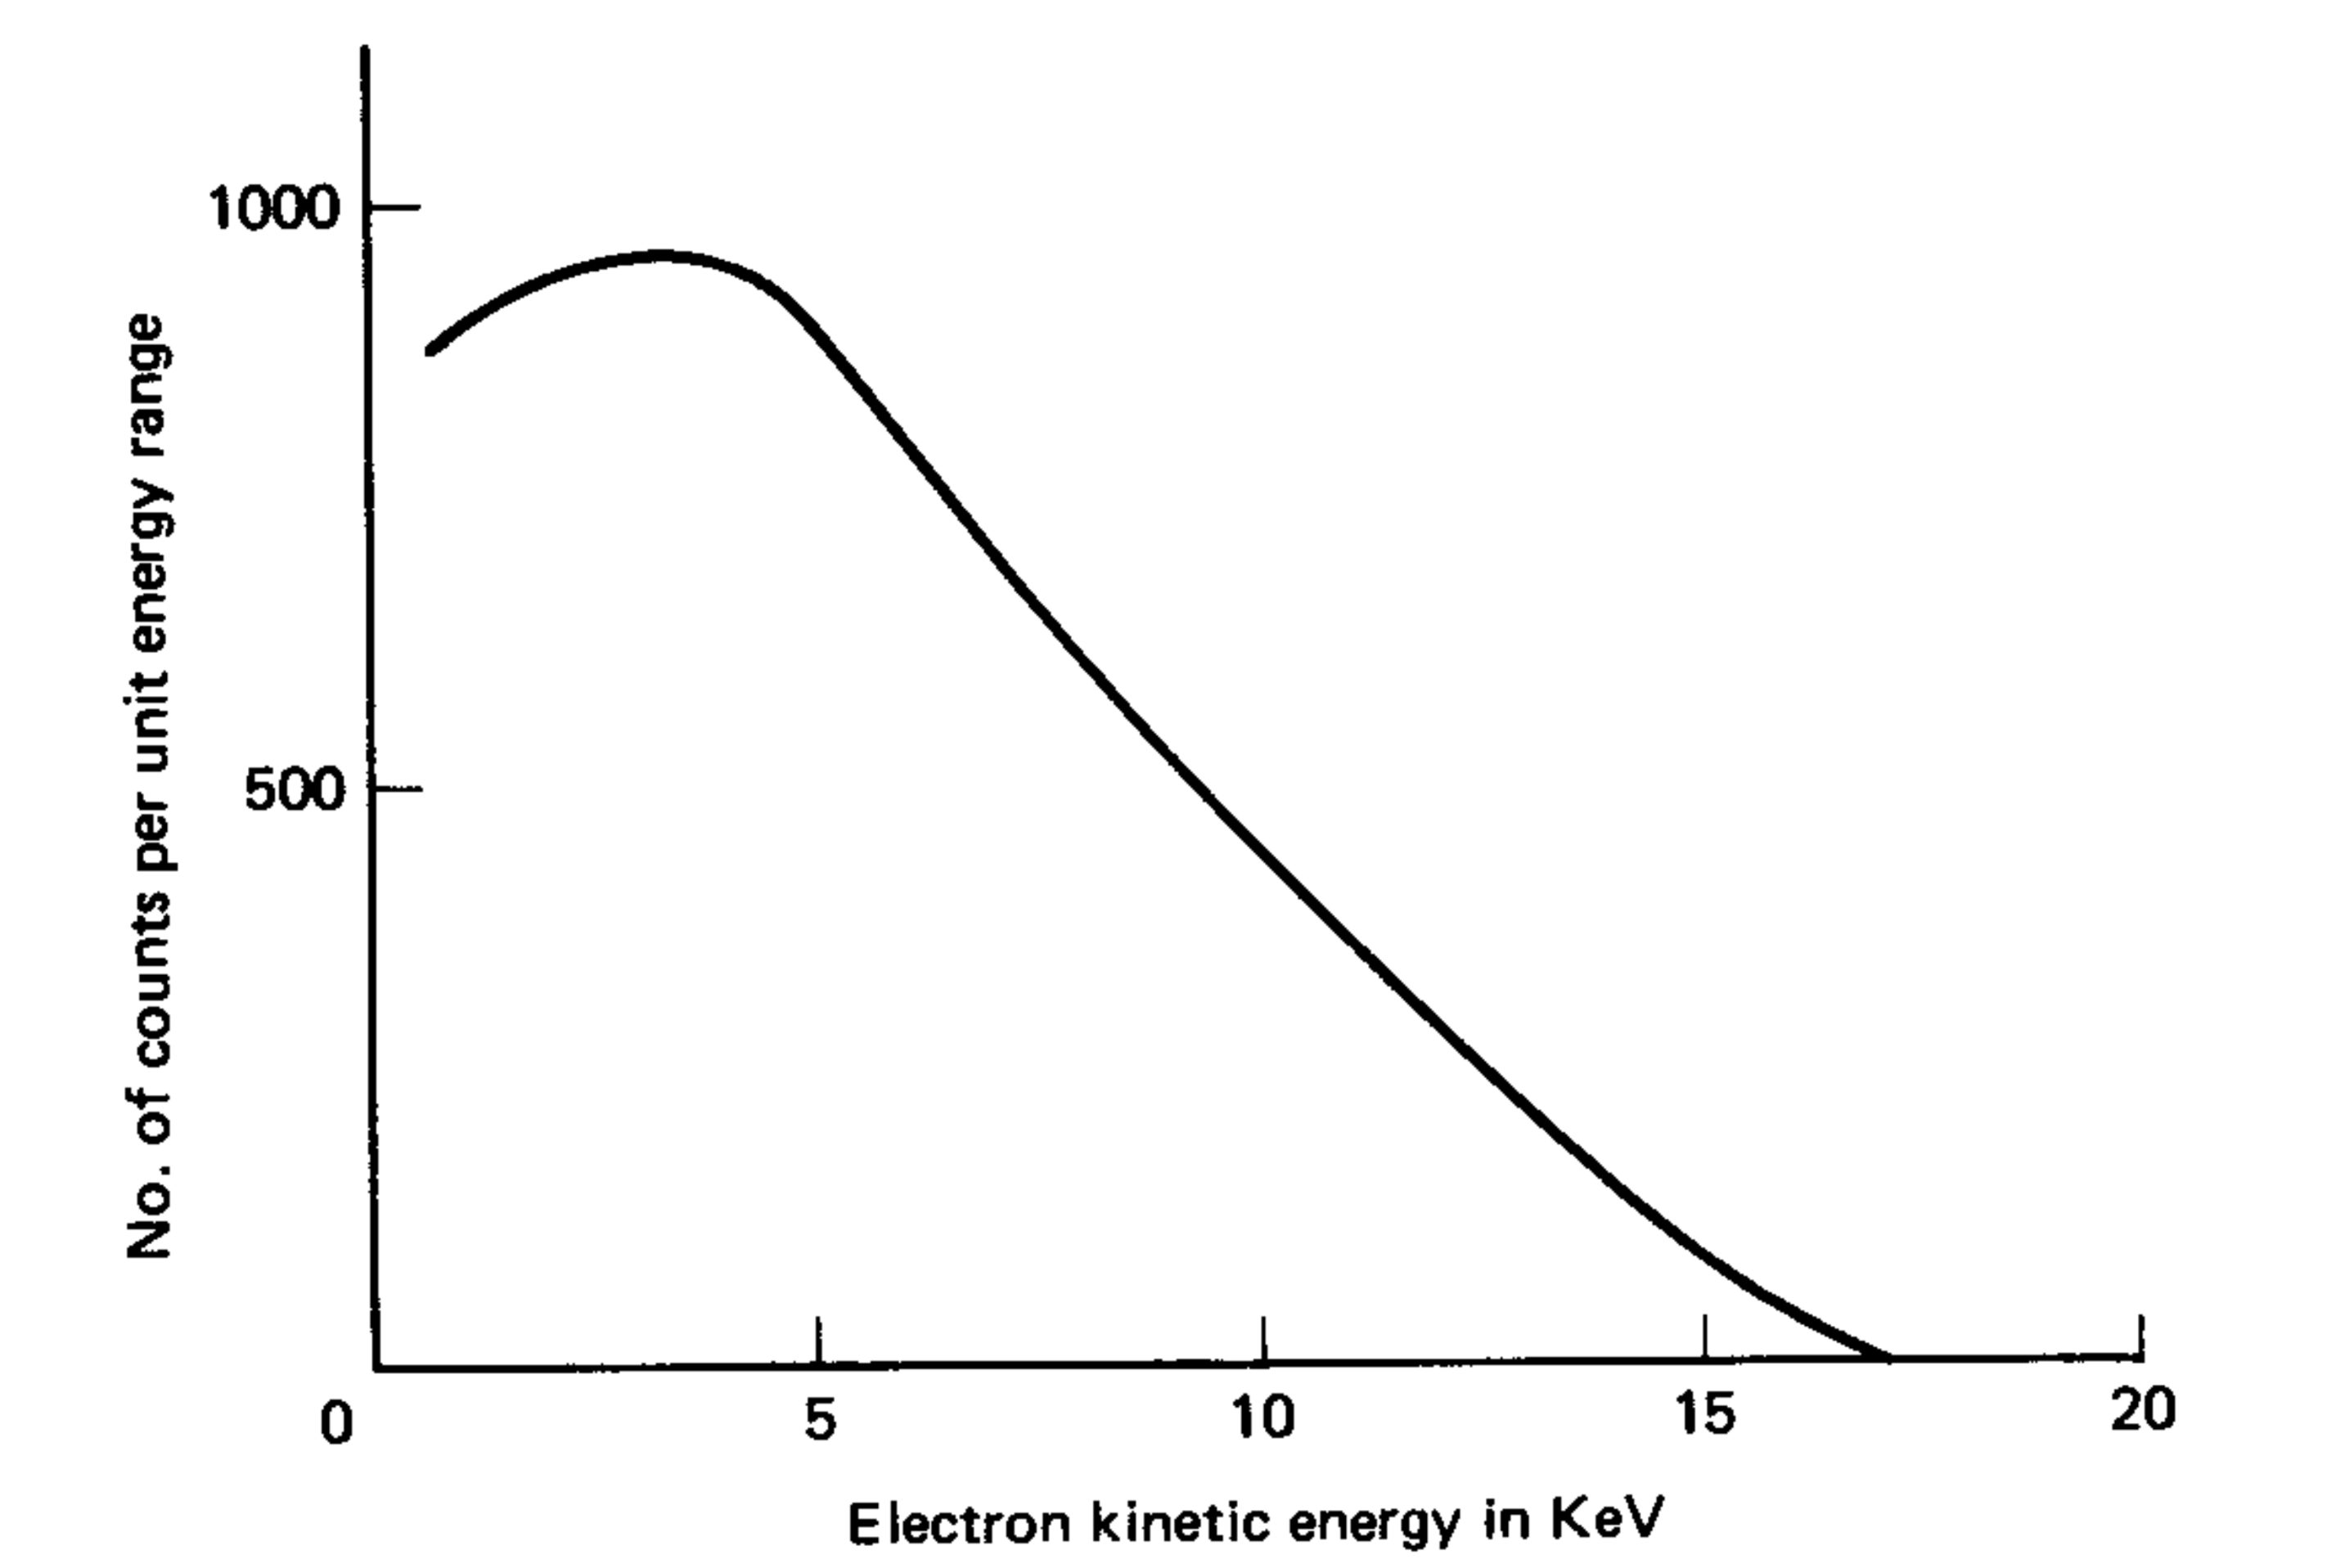
\includegraphics[scale=0.3]{Figures/electron_beta_decay_spectrum.pdf}
		\caption[The beta decay spectrum of tritium]{ {\textbf{The beta decay spectrum of tritium}} \\The figure shows the electron energy spectrum in a beta decay of tritium \cite{griffiths}.}
		\label{figure_the_beta_decay_spectrum_of_tritium}	
	\end{center}
\end{figure}
%

In 1930, Wolfgang Pauli proposed that the beta decay was not a two-body decay, but a three-body decay. He predicted that the third particle proposed by him would be neutral and light. Pauli originally named it neutron. Later, with Chadwick's discovery of the neutron, Fermi changed the name of his predicted particle to neutrino \cite{griffiths}. A few years later, in 1933, Pauli and Perrin proposed that neutrinos were massless \cite{griffiths}.

\subsection{The First Neutrino Measurement}
It was not until 1956 that neutrinos were experimentally verified by Cowan and Reines. They conducted an experiment at the Savannah River nuclear reactor in South Carolina that consisted of a big tank of water and cadmium chloride, surrounded by 4,200 litters of liquid scintillator, seated near the nuclear reactor. If neutrinos, as predicted by Pauli, were real, they would be produced by the nuclear reaction inside the reactor and, as entering the detector, would possibly hit the protons of the water and produce a positron and a neutron. This reaction is called inverse beta decay, and it is given as:
%
\begin{equation}
	\overline{\nu} + p^+ \longrightarrow n + e^+.
	\label{inverse_beta_decay_eq}
\end{equation}
%
The reaction's signature they were looking for were two photons, produced by the electron-positron annihilation, and, a few microseconds later, a few photons, produced by the neutron capture by the cadmium \cite{nobel_leptons}. They published their results in a paper called “Detection of the Free Neutrino: A Confirmation”, confirming the existence of neutrinos (Ref. \cite{cowan_reines}). 


\section{Different Types of Neutrinos}
In 1953, Konopinski  and Mahmoud proposed the existence of a lepton number and the conversation of it, which could explain why certain reactions happen and some others do not. As convention, it was established that leptons would have a lepton number L = 1, that antileptons would have lepton number L = $-$1, and that any other particle would have lepton number L = 0. By this rule, an antineutrino should be produced in a beta decay. Although the rule explained why many reactions supposedly allowed to happen were not observed, it still did not explain a few cases. This led them to postulate the existence of a lepton number for each of the leptons. That is, a muon number, an electron number and, years later, a tau number (see table \ref{lepton_family}) \cite{Konopinski_Mahmoud}. 
%
\begin{table}
	\begin{center}
		\begin{tabular}{cccc}
			\bottomrule
						& \textbf{Lepton number}	&	\textbf{Electron number}	&	\textbf{Muon number}\\
			\toprule
			Leptons			&		&		&	 \\
			$e^-$			&	1	&	1	&	0\\ 
			$\nu_e$			&	1	&	1	&	0\\
			$\mu^-$			&	1	&	0	&	1\\	
			$\nu_\mu$		&	1	&	0	&	1\\
			Antileptons		&		&		&	  \\
			$e^+$			&	$-$1	&	$-$1	&	0\\	
			$\overline{\nu_e}$	&	$-$1	&	$-$1	&	0\\
			$\mu^-$			&	$-$1	&	0	&	$-$1\\
			$\nu_\mu$		&	$-$1	&	0	&	$-$1\\
			\toprule
		\end{tabular}
		\caption[The lepton family]{{\textbf{The lepton family from 1962 to 1976}} \cite{griffiths}}
		\label{lepton_family}
	\end{center}
\end{table}
\newline

This hypothesis was experimentally checked in 1962 at the Brookhaven National Laboratory by Lederman, Schwartz e Steinberger. Their experiment consisted of having a beam of charged pions, produced in a particle accelerator called Alternating Gradient Synchrotron (AGS), and observing the neutrinos that accompanied the muons produced whenever the beam pions decayed. Hypothetically, if the lepton number is the same for muons and electrons, the following reactions are allowed and, consequently, should be observed: 
%
\begin{equation}
	\nu_{\mu} + n \longrightarrow p + e^-
	\label{lss_primeira}
\end{equation}

\begin{equation}
	\overline{\nu}_{\mu} + p \longrightarrow n + e^+
	\label{lss_segunda}
\end{equation}

\begin{equation}
	\nu_{\mu} + n \longrightarrow p + \mu^-
	\label{lss_terceira}
\end{equation}
 
\begin{equation}
	\overline{\nu}_{\mu} + p \longrightarrow n + \mu^+
	\label{lss_quarta}
\end{equation}
%
In the experiment only the third and fourth reactions were observed, implying that the interaction of neutrinos produced with a muon can only produce other muons. That is, each lepton has a corresponding neutrino \cite{two_neutrinos}.

\subsection{The Solar Neutrinos Flux Problem}
The series of nuclear reactions occurring in the solar and stellar cores are given by the so-called carbon–nitrogen–oxygen (CNO) cycle and the pp-chain. In the CNO cycle the four protons are successively absorbed in a series of nuclei, starting and ending with carbon. In the pp-chain two protons combine to form the deuteron and further protons are added \cite{the_story_of_the_neutrino}. In either case, the net process is:
%
\begin{equation}
	p+p+p+p \longrightarrow He^4 +e^+ + e^+ +\nu_e +\nu_e
	\label{solar_reaction}
\end{equation}
%
Ray Davis proposed an experiment to measure the neutrinos emitted by the sun. The experiment was based on the following inverse beta decay.
%
\begin{equation}
		\nu_e + Cl^{37} \longrightarrow e^- +Ar^{37}
		\label{solar_reaction}
\end{equation}
%
The main idea was that the chlorine would absorb a solar neutrino and would produce an electron and an Ar$^{37}$. A tank containing 615 tons of a fluid rich in chlorine called tetrachloroethylene was placed in the Homestake gold mine in South Dakota. The fluid was periodically purged with Helium gas to remove the argon-37 atoms, which were then counted by means of their radioactivity. In the average, the experiment measured one neutrino after every three days and ran for 30 years. Although the measurement of solar neutrinos was a success, the experiment measured a flux 2/3 smaller than the one theoretically predicted by John Bahcall. This difference became known as the solar neutrino problem and the results were published in 1970 \cite{the_story_of_the_neutrino}.

\subsection{Neutrino Oscillation}

In 1967 Bruno Pontecorvo published a paper called ``Neutrino Experiments and The Problem of Conservation of Leptonic Charge" in which he discussed the effect of neutrino oscillations for the solar neutrinos. He wrote \cite{pontecorvo_1967}: 
\begin{quote}
\emph{``From an observational point of view the ideal object is the sun. If the oscillation length is smaller than the radius of the sun region effectively producing neutrinos, direct oscillations will be smeared out and unobservable. The only effect on the earth’s surface would be that the flux of observable sun neutrinos must be two times smaller than the total (active and sterile) neutrino flux."}
\end{quote}
%
Thus, Pontecorvo anticipated the solar neutrino problem! 

The next paper about neutrino oscillations was published two years later by V. Gribov and B. Pontecorvo. They considered a scheme of neutrino mixing and oscillations with four neutrino and antineutrino states: two left-handed states of neutrinos, $\nu_e$ and $\nu_\mu$, and two right-handed states of antineutrinos,  $\overline{\nu}_e$ and $\overline{\nu}_\mu$. The main assumption of Gribov and Pontecorvo was that there are no sterile neutrino states \cite{neutrino_oscillations_brief_history_and_present_status}.

\subsection{Current Neutrino Oscillation Model}

The current model of oscillations considers three neutrinos: The electron neutrino, the muon neutrino and the tau\footnote{The tau neutrino particle was detected in 1997 by The Direct Observation of NU Tau (DONuT) experiment at Fermi National Laboratory (Fermilab) \cite{tau_neutrino_discovery}.} 

In this model, a neutrino flavor eigenstate with momentum $\vec{p}$ can be written as a linear combination of the neutrino mass eigenstates:
%
\begin{equation}
	|\nu_\alpha \rangle = \sum_{k=1}^n U^*_{\alpha k} |\nu_k \rangle,
	\label{nu_state}
\end{equation}
%
Where $\alpha = e, \mu, \tau$; $|\nu_k\rangle$ is the mass base, $k$ is the known mass states and $U$ is the Pontecorvo-Maki-Nakagawa-Sakata (PMNS) matrix \cite{MNS, PMNS}, that is:
%
\begin{equation}
	U = \left( \begin{array}{ccc} 
	1 & 0 & 0 \\ 
	0 & c_{23} & s_{23} \\
	0 & -s_{23} & c_{23} \end{array} \right)
	%
	\left(\begin{array}{ccc} 
	c_{13} & 0 & s_{13}e^{-i\delta} \\ 
	0 & 1 & 0 \\ 
	-s_{13}e^{+i\delta} & 0 & c_{13} \end{array}\right)
	%
	\left(\begin{array}{ccc}
	c_{12} & s_{12} & 0 \\ 
	-s_{12} & c_{12} & 0 \\ 
	0 & 0 & 1 \end{array} \right)
	%
	\label{PMNS_factored}
\end{equation}
%
where $c_{ij} \equiv \cos(\theta_{ij}), \ s_{ij} \equiv \text{sen}(\theta_{ij})$ and $\delta$ is the Charge Parity (CP) symmetry violating phase parameter.
In equation \ref{PMNS_factored}, the three matrices represent different neutrino oscillation sectors. The left matrix represents the accelerator neutrino sector, the middle matrix represents the transition $\nu_e \rightarrow \nu_\tau$, that is present in both accelerator and reactor neutrino sectors, and the right matrix represents the reactor neutrino sector.

Consider that the flavor eigenstates are orthogonal, that the mass eigenstates are also orthogonal, that the PMNS matrix is unitary, that the neutrinos are oscillating in the vacuum, and also that the mass eigenstates are hamiltonian's eigenstates. The last statement leads to:
%
\begin{equation}
	H|\nu_k \rangle = E_k |\nu_k \rangle
	\label{nu_schrodinger}
\end{equation}
%
That means that the energy eigenvalues are
%
\begin{equation}
	E_k = \sqrt{\vec{p}^2 + m_k^2}.
	\label{nu_energy}
\end{equation}
%
If we evolve the mass eigenstate in time, it is possible to write the flavor eigenstate as
%
\begin{equation}
	|\nu_\alpha (t) \rangle = \sum_{k=1}^n U^*_{\alpha k} e^{-iE_kt}|\nu_k \rangle.
	\label{nu_state_time}
\end{equation}
%
Rewriting equation \ref{nu_state_time} only in the flavor base yields 
%
\begin{equation}
	|\nu_\alpha (t)\rangle = \sum_{\beta = e, \mu, \tau} \left( \sum_{k=1}^n U^*_{\alpha k} U_{\beta k} e^{-iE_kt} \right) |\nu_\beta \rangle.
	\label{nu_state_time_2}
\end{equation}
%

The term between parenthesis is the $\nu_\alpha \rightarrow \nu_\beta$ transition amplitude. With that information and some more algebra it is possible to show that the time dependent transition probability is
\begin{equation}
	P_{\nu_\alpha \rightarrow \nu_\beta}(t) = \sum_{k=1}^n \sum_{j=1}^n U^*_{\alpha k} U_{\beta k} U_{\alpha j} U^*_{\beta j} e^{i(E_k - E_j)t}.
	\label{transition_probability}
\end{equation}

Some approximations and simplifications are possible. As neutrino masses are extremely small, they are in a relativistic regime. This allow the approximation, through Taylor expansion 
%
\begin{equation}
	E_k - E_j \approx \frac{m^2_k - m^2_j}{2E} = \frac{\Delta m^2_{kj}}{2E}.
	\label{nu_Ej-Ek}
\end{equation}
%
As neutrino's velocity is close to the light's one in vaccum 
%
\begin{equation}
	L \approx ct = t.
	\label{nu_L}
\end{equation}
%
Separating the exponential in the equation \ref{transition_probability} into real and imaginary parts, the indexes in $k=j$ and $k>j$, and using some more algebra the final result is
%
\begin{eqnarray}
	P_{\nu_\alpha \rightarrow \nu_\beta} (L/E) & = & \delta_{\alpha\beta} - 4\sum_{k>j}^n  \mathfrak{Re}[U^*_{\alpha k} U_{\beta k} U_{\alpha j} U^*_{\beta j}]\text{ sen}^2\left(\frac{\Delta m^2_{kj} L}{4E} \right) \nonumber \\
	& \quad & + \ 2\sum_{k>j}^n\mathfrak{Im}[U^*_{\alpha k} U_{\beta k} U_{\alpha j} U^*_{\beta j}]\text{ sen}\left(\frac{\Delta m^2_{kj} L}{2E} \right).
	\label{nu_oscillation_final}
\end{eqnarray}
%

In figure \ref{fig:nu_osc_prob}, you will find a plot for the three flavor oscillation probabilities as a function of $L/E_{\nu}$, assuming the original state is $\nu_{\mu}$

\begin{figure}[h!]
	\begin{center}
		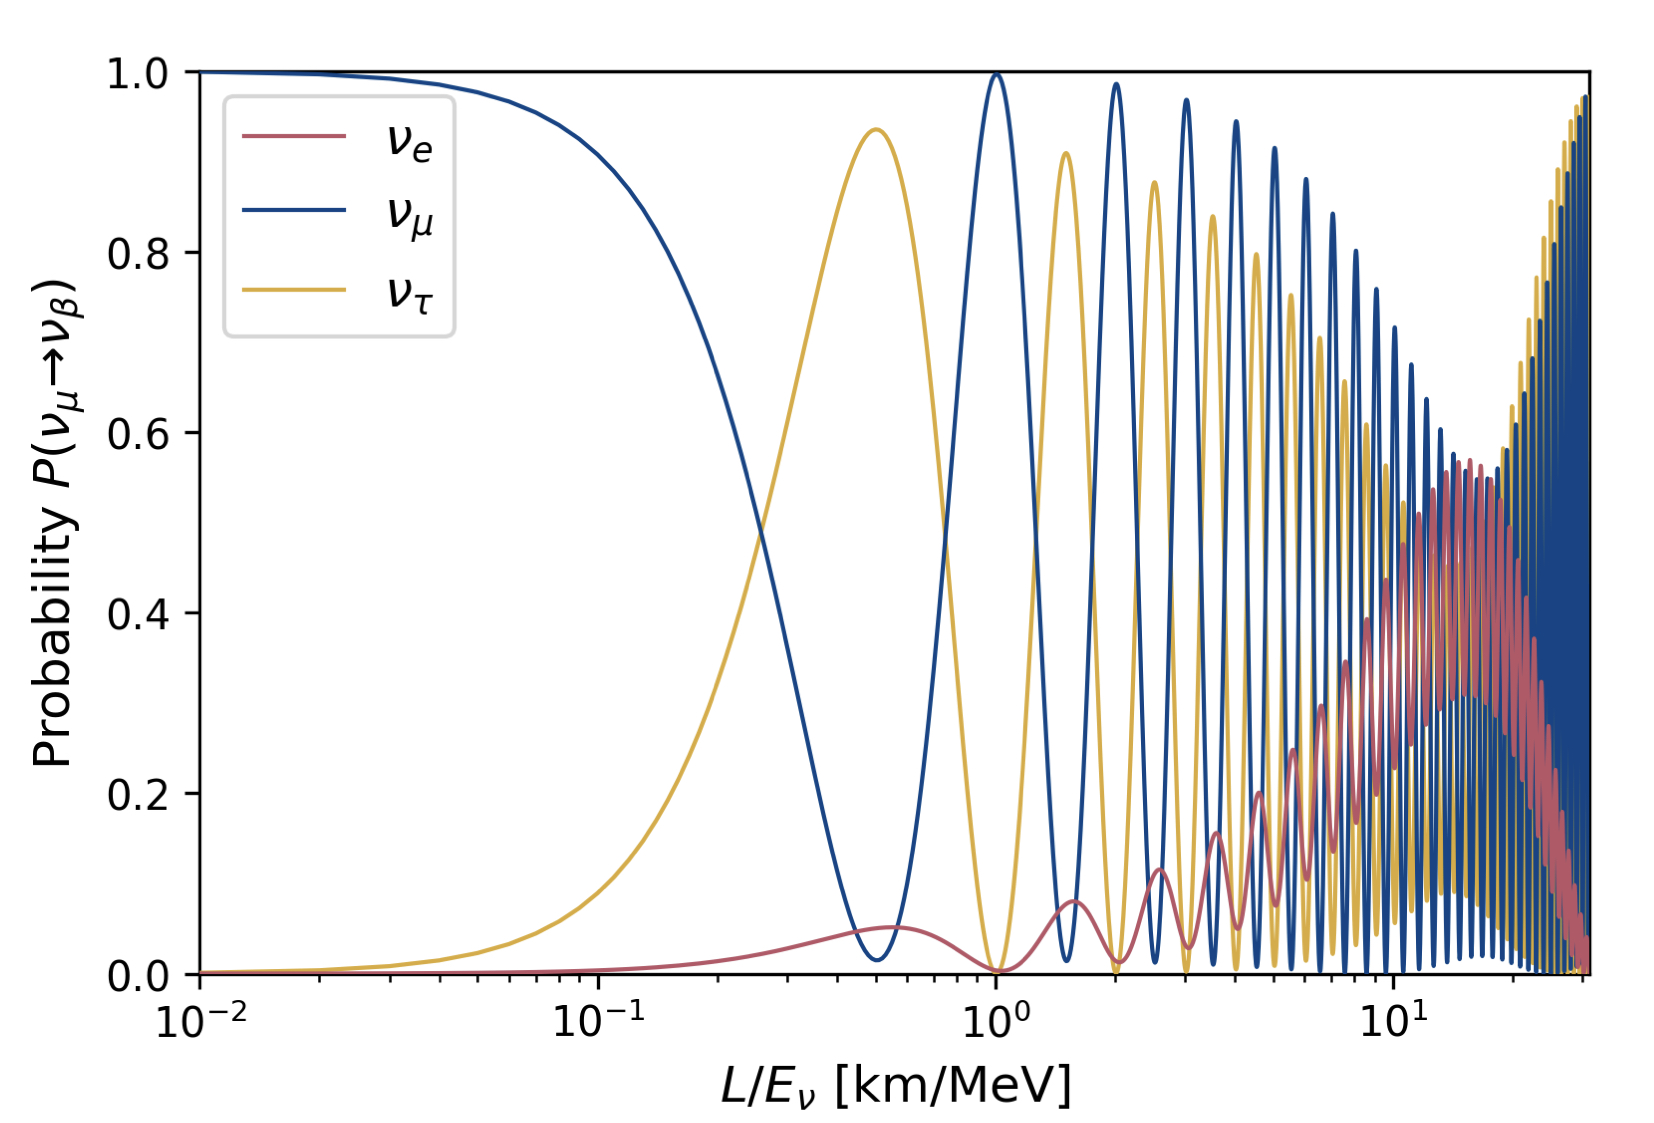
\includegraphics[scale=0.2]{Figures/three_flavor_osc.jpg}
		\caption[Three Flavor Oscillation Model]{\textbf{Three Flavor Oscillation Probabilities as a Function of L/E$_{\nu}$} \\Three Flavor Oscillation Probabilities as a Function of L/E$_{\nu}$, assuming the original state is $\nu_{\mu}$, \cite{Lauren_thesis}.}
		\label{fig:nu_osc_prob}
	\end{center}
\end{figure}

For the antineutrinos, the mathematical steps are similar from the ones we just took \cite{oscillation_math}. 

\subsubsection{First Neutrino Oscillation Measurements}
The first oscillation measurements, and consequently the confirmation that neutrinos have mass, were made by the Super-Kamiokande experiment. The Super-Kamiokande detector is located 1 km underground in the Kamioka-mine, Hida-city, Gifu, Japan. It consists of a stainless-steel tank, with 39.3 m of diameter and 41.4 m tall, filled with 50,000 tons of ultra pure water. It has about of 13,000 photo-multipliers installed on the tank's wall (see image \ref{superk_picture}).
In 1998 the Super-Kamiokande collaboration published the first neutrino oscillation measurements in a paper called ``Evidence for oscillation of atmospheric neutrinos" \cite{first_kamioka_measure}.
%
\begin{figure}[h!]
	\begin{center}
		\includegraphics[scale=0.5]{Figures/superk.pdf}
		\caption[Inside Super-Kamiokande tank]{ {\textbf{Inside Super-Kamiokande tank}}\\Workers doing photomultipliers (PMTs) checking inside Super-Kamiokande detector \cite{superk_picture}.}
		\label{superk_picture}	
	\end{center}
\end{figure}
%

\section{Current Understanding of Neutrino Physics}

At this point, allow me to briefly summarize the understanding we currently have of neutrinos, obtained through the experiments and studies I mentioned above and also by many other experiments I left out from this historical overview. 

Neutrinos are chargeless leptons with small non-zero mass that only interact through the weak force. So far, we know of the existence of three types of them, that we call "flavor", and that are named after the charged lepton that accompanies them in charged-current weak interactions: electron neutrino ($\nu_e$), muon neutrino ($\nu_{\mu}$), and tau neutrino ($\nu_{\tau}$). 

The weak interaction is mediated by three bosons: The $Z^{0}$ boson, responsible for carrying the Neutral Current (NC) interactions, and the $W^{-}$ and $W^{+}$ bosons, responsible for carrying the Charged Current (CC) interactions. The Feymann Diagrams below represent said interactions. In the CC neutrino interactions, we have an incoming neutrino interacting with a nucleus' quark and producing a charged lepton, their neutrino counterpart, and a different nucleus' quark, such as to conserve charge number. In the NC the incoming and outgoing particle natures remain the same, but transfer momentum and energy. 

\begin{figure}[h!]
	\begin{center}
		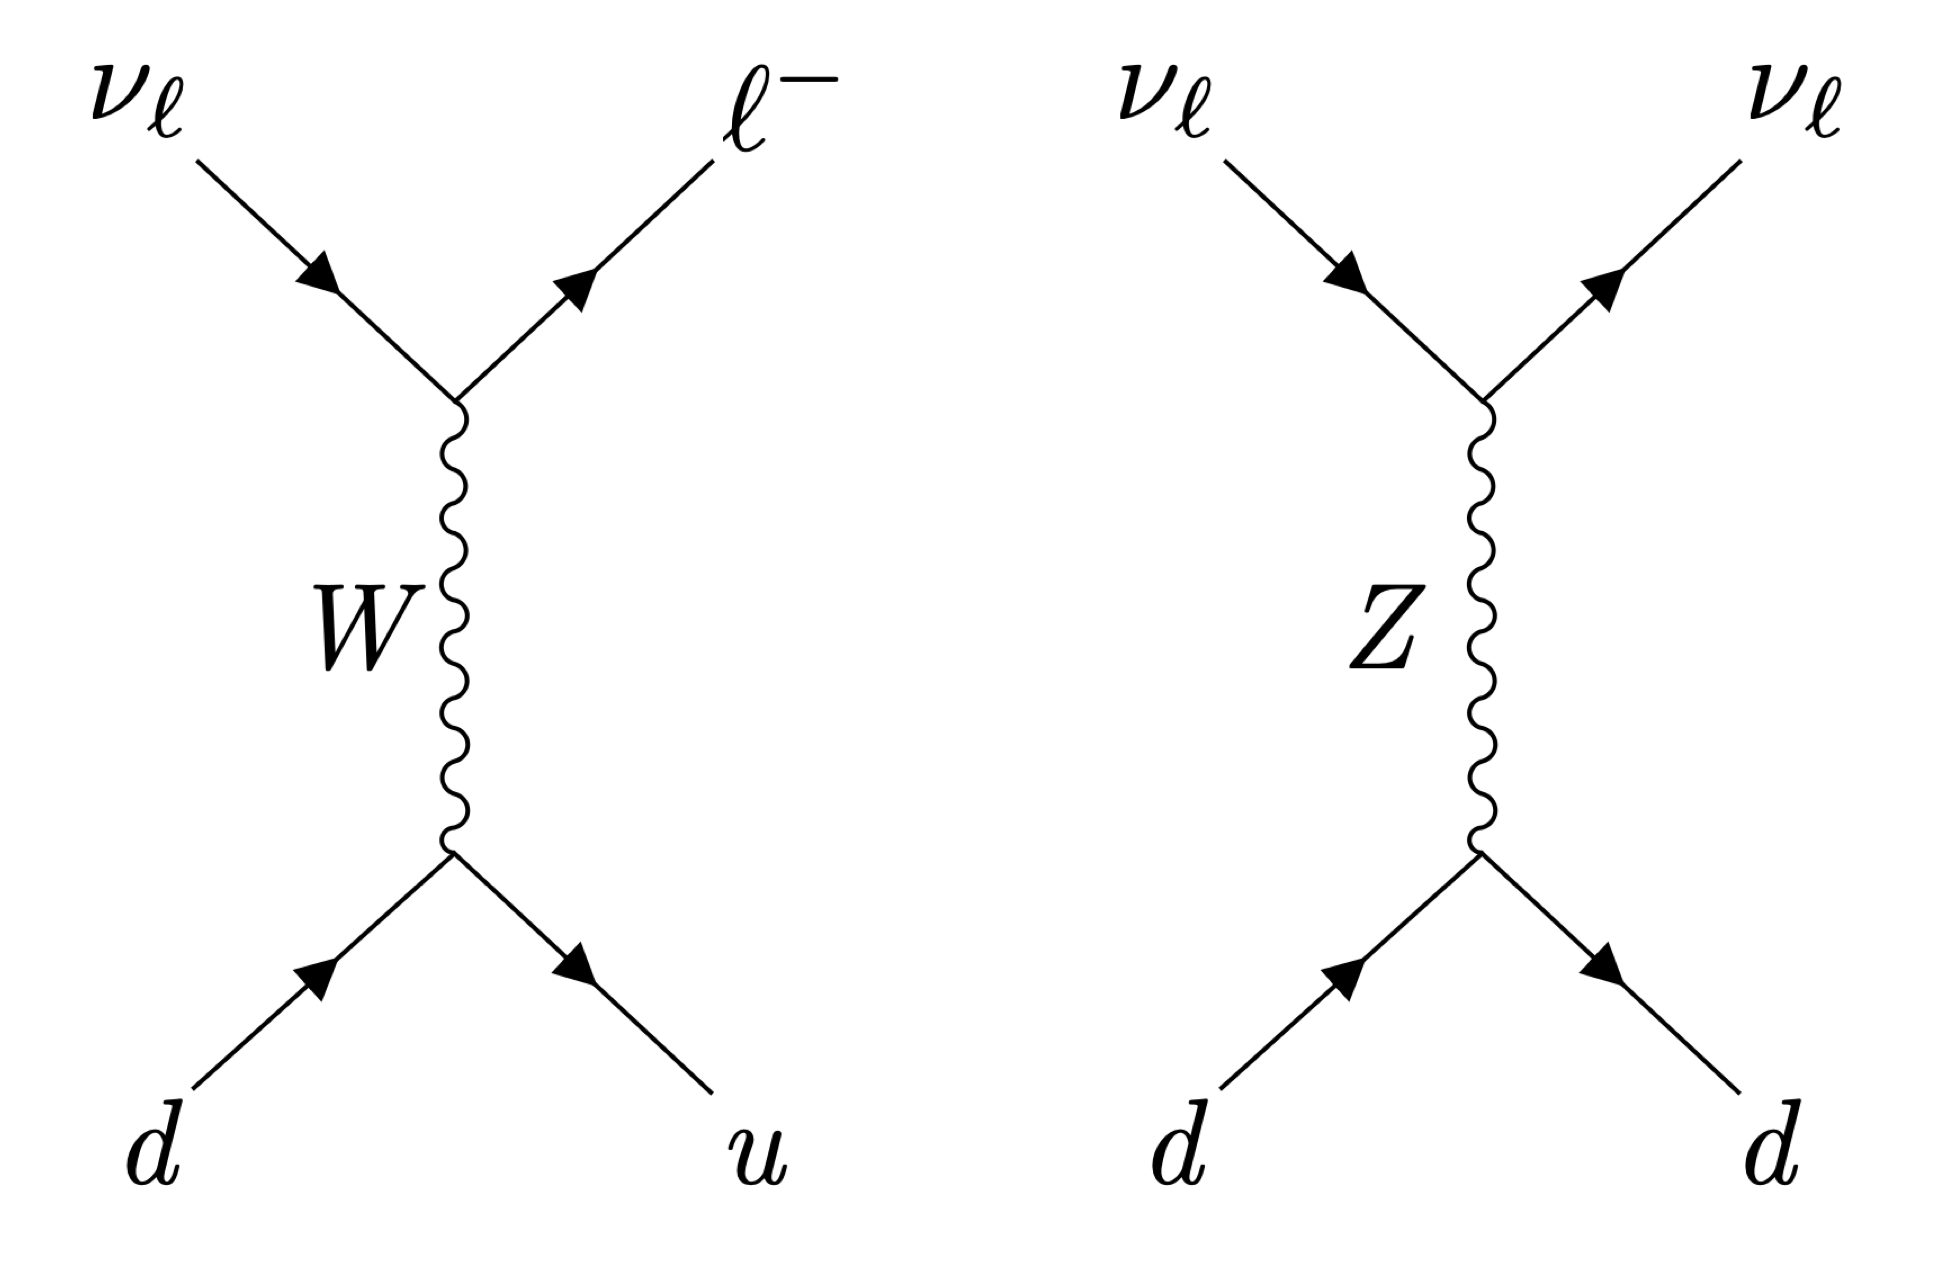
\includegraphics[scale=0.3]{Figures/feymann_diag.jpg}
		\caption[Feymann Diagrams for the two types of weak interactions]{ {\textbf{Feymann Diagrams for the two types of weak interactions}} \\ On the left, the Feymman diagram for a Charged Current interaction, carried by a W boson. On the right, the Feymman diagram for a Neutral Current interaction, carried by a Z boson, \cite{Lauren_thesis}.}
		\label{feymann_diag}	
	\end{center}
\end{figure}

We can observe different outcome final products from neutrino interactions, depending on the energy of the incoming neutrino. At lower energies, $\lessapprox 10$ GeV, the dominant processes will be quasi-elastic scattering (QE), where neutrinos scatter off of a nucleon, and resonance, where neutrinos scatter off of a nucleon that gets excited and decays. From $10$ GeV beyond, the dominant procress is Deep Inelastic Scattering (DIS) where neutrinos scatter directly off of nucleus' quarks.In figure \ref{nu_scatter} you can see a summary of the existing measurements of CC neutrino cross-section divided by neutrino energy and plotted as a function of energy. 

\begin{figure}[h!]
	\begin{center}
		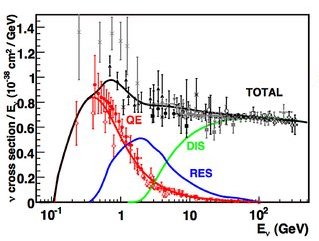
\includegraphics[scale=0.9]{Figures/nu_scatter.jpg}
		\caption[Total CC neutrino cross-section per nucleon as function of energy]{ {\textbf{Total CC neutrino cross-section per nucleon as function of energy}} \\ Summary of the existing measurements of CC neutrino-nucleon cross-section divided by neutrino energy and plotted as a function of energy. The QE is in red, the resonance in blue, the DIS in green, and the black is the total cross-section, when considering all the previous processes \cite{nu_scatter_zeller}.}
		\label{nu_scatter}	
	\end{center}
\end{figure}


%<<<<<<<<<<<<<<<<<<<<<<<<<<<<< Change Feymann Diagrams here!!! >>>>>>>>>>>>>>>>>>>>>>>>>>>>>>>>>>>>>

\subsubsection{The CP Symmetry Violating Phase Parameter}

The $\delta$ parameter showed in the PMNS matrix in equation \ref{PMNS_factored} quantifies the charge conjugation and parity symmetry violation. The strong and electromagnetic interactions are invariant under CP symmetry, but some weak interaction processes are not. This violating phase parameter is also observed in the quark sector and was already measured. The CP symmetry violating phase parameter is still not observed in the lepton sector.

\subsubsection{The Character of the Neutrino Mass Spectrum (Mass Hierarchy)}

The equation \ref{nu_oscillation_final} limits that the data of neutrino oscillation experiments can only measure the mass-squared differences. Due to the tremendous growth of the neutrino experiment efforts in the past two decades, it is known that \cite{delta_2_1}
%
\begin{equation}
	\Delta m^2_{21} = (7.53 \pm 0.18) \times 10^{-5} \ \text{eV}^2
	\label{delta_21}
\end{equation}
%
and \cite{delta_3_2}
%
\begin{equation}
	\Delta m^2_{32} = (2.34 \pm 0.09) \times 10^{-3} \ \text{eV}^2
	\label{delta_32_normal}
\end{equation}
%
or 
%
\begin{equation}
	\Delta m^2_{32} = (-2.37^{+0.07}_{-0.11}) \times 10^{-3} \ \text{eV}^2.
	\label{delta_32_inverted}
\end{equation}
%
The relative ordering $m_1 < m_2$ is known through observations of solar neutrinos, which are subject to resonant matter effects in the sun \cite{delta_2_1}. The value in \ref{delta_32_normal} corresponds to what is called Normal Hierarchy and \ref{delta_32_inverted} to what is called Inverted Hierarchy. Normal hierarchy is the condition where the $m_1 < m_2 < m_3$. Inverted hierarchy is the condition where the $m_3 < m_1 < m_2$. A schematic of the normal and inverted hierarchies can be found on figure \ref{mass_hierarchy}. The precision of neutrino sector measurements has reached a point where the unknown hierarchy is a major hurdle to further progress \cite{prospects_patterson}.

\begin{figure}
	\begin{center}
		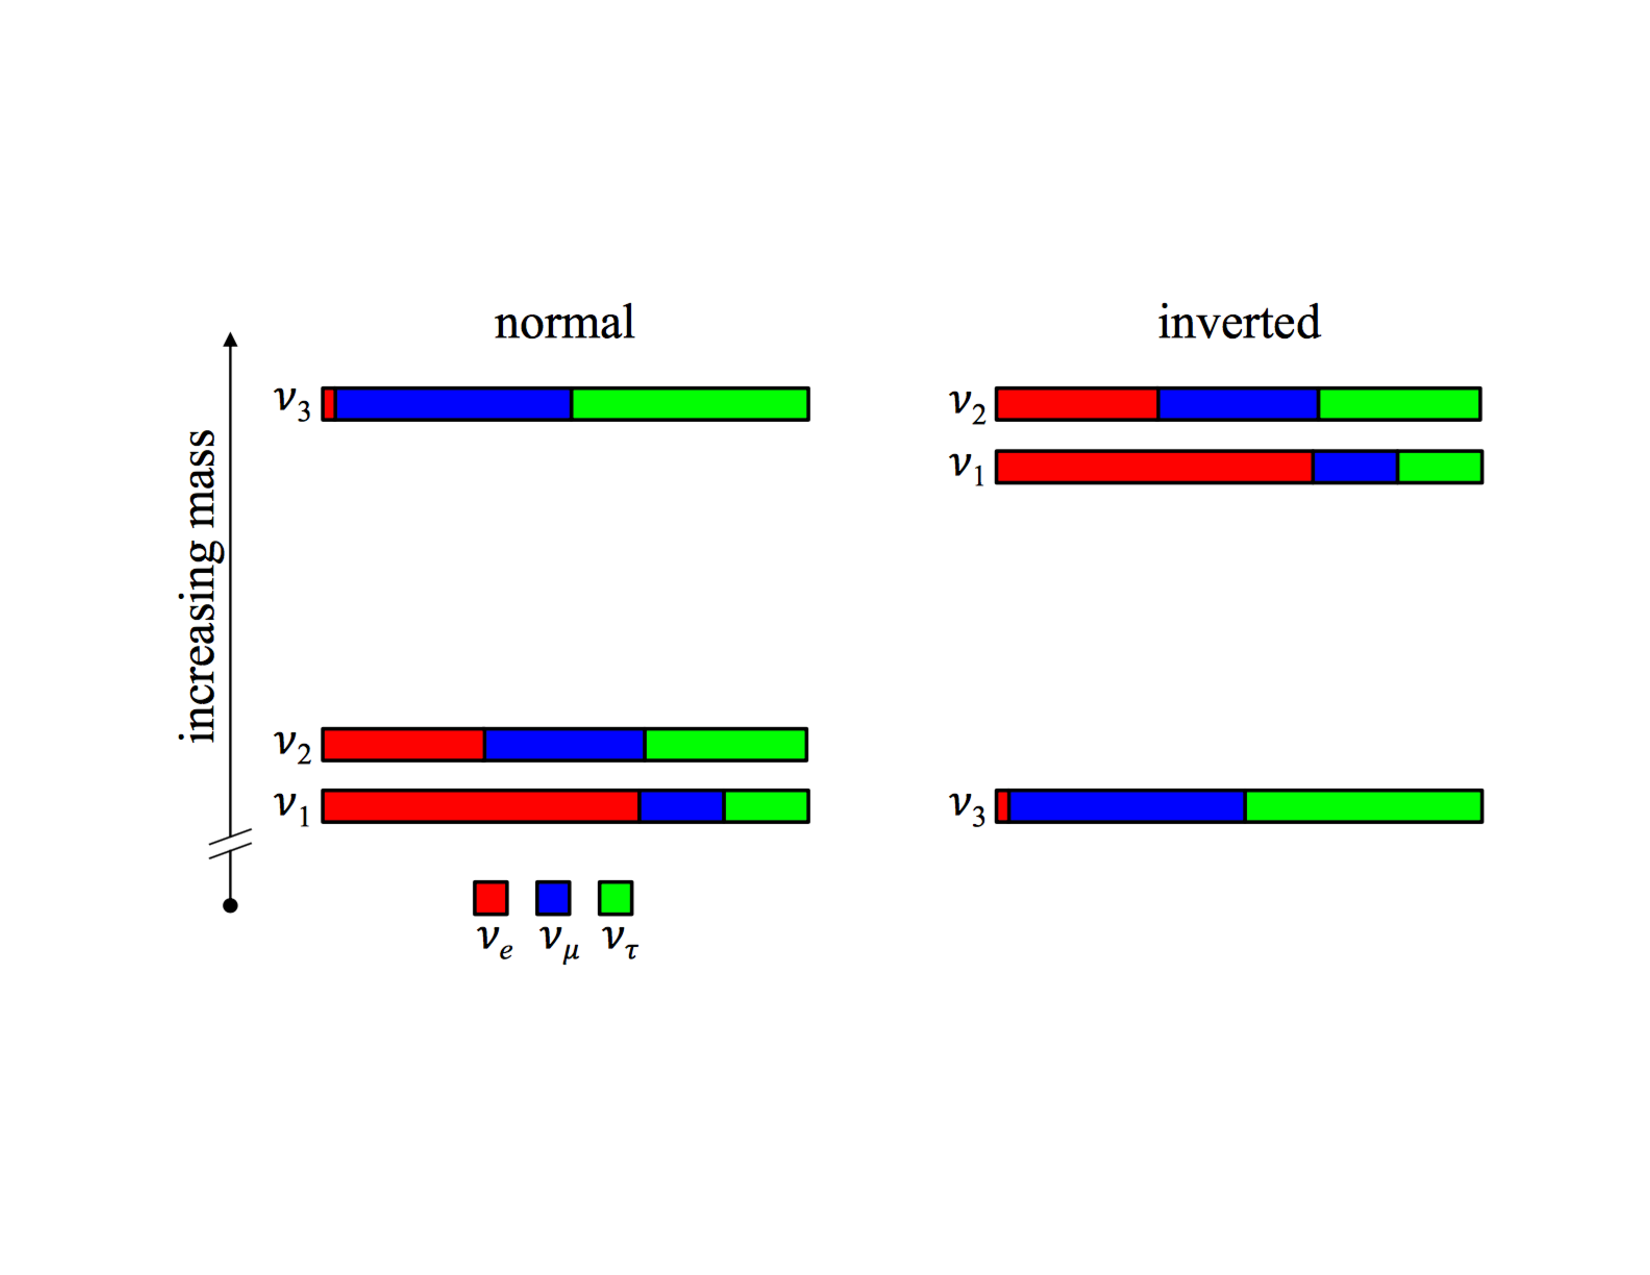
\includegraphics[scale=0.5]{Figures/mass_hierarchy.pdf}
		\caption[The Mass Hierarchy]{ {\textbf{The Mass Hierarchy}}\\The two possible neutrino mass hierarchies. The colors represent the approximate flavor admixtures present in each mass eigenstate \cite{prospects_patterson}.}
		\label{mass_hierarchy}	
	\end{center}
\end{figure}

\subsubsection{The $\mathbf{\theta_{23}}$ Octant Definition Problem}

The $\theta_{23}$ parameter is present is both $P_{\nu_\mu \rightarrow \nu_\mu}$ and $P_{\nu_\mu \rightarrow \nu_e}$ calculations. Most of the near past neutrino experiments take advantage of an approximation that considers the existence of only two neutrino flavors due to limitations in their resolution. In this approximation the oscillation probabilities take the form of
%
\begin{equation}
	P_{\nu_\mu \rightarrow \nu_e} \propto \text{sin}^2(2\theta_{23}) \ \text{ and } \ P_{\nu_\mu \rightarrow \nu_\mu} \propto \text{sin}^2(2\theta_{23}),
	\nonumber
\end{equation}
%
which implies in a redundancy in the value of $\theta_{23}$, with the possibilities being either $\theta_{23} > \pi/4$ or $\theta_{23} < \pi/4$. 
In more recent results, experiments such as NuMI Off-axis $\nu_e$ Appearance (NO$\nu$A), Main Injector Neutrino Oscillation (MINOS) and Tokai to Kamioka (T2K), do not use this approximation, resulting in a 2 fold degeneracy solution for the mixing angle $\theta_{23}$. The latest results were presented by the NO$\nu$A Collaboration and can be seen in figure \ref{nova_result}, which shows the two best fit values with their 90\% confidence level contours. In this study, NO$\nu$A Collaboration disfavored the maximal mixing ($sin^2 \theta_{23} = 0.5$) scenario with $2.6 \sigma$ significance \cite{NOVA}.

\begin{figure}
	\begin{center}
		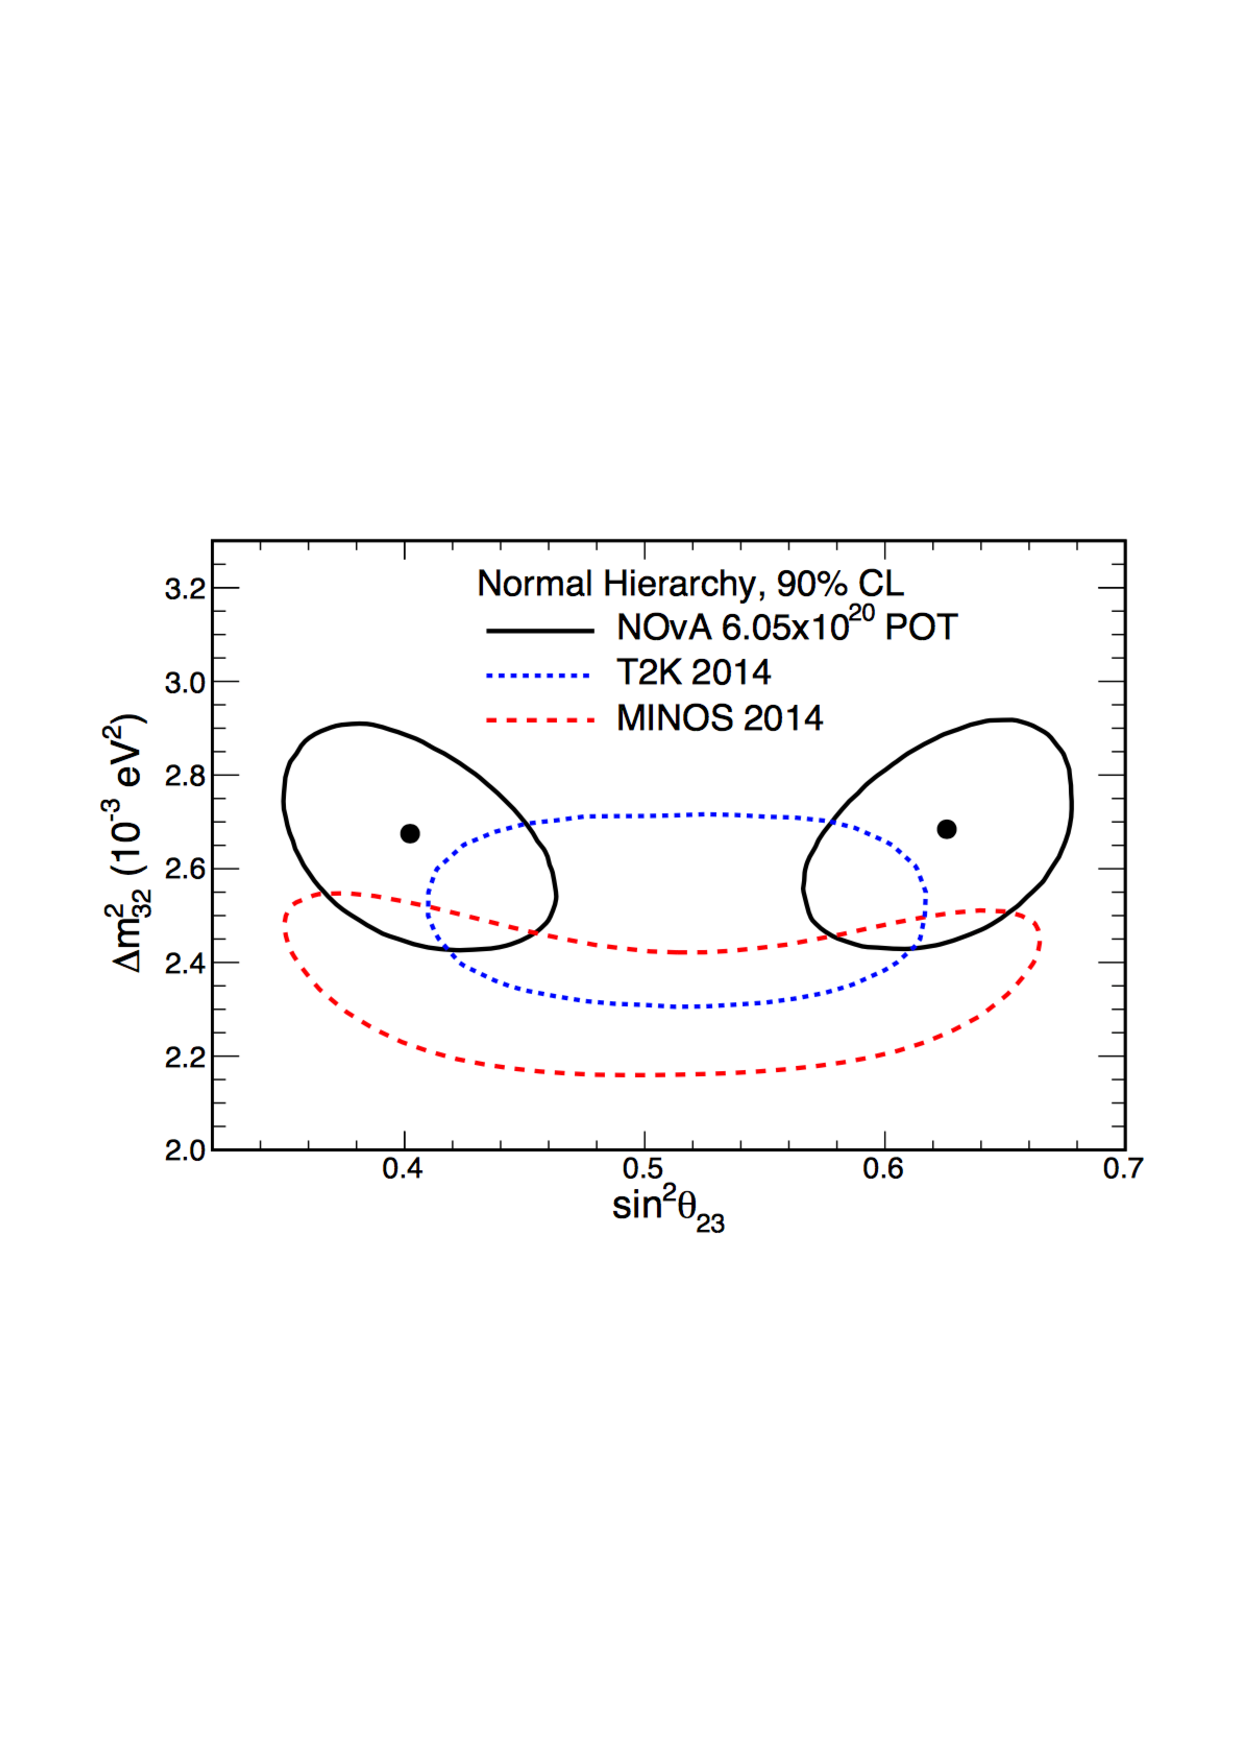
\includegraphics[scale=0.7]{Figures/nova_result.pdf}
		\caption[Preliminary $\theta_{23}$ results from the NO$\nu$A Experiment]{ {\textbf{Preliminary $\theta_{23}$ results from the NO$\nu$A Experiment}} \\ Best fit (black dots) and allowed $90\%$ confidence level regions (solid black curves) of $\sin^2 \theta_{23}$ and $\Delta m^2_{23}$ for the normal hierarchy. The dashed curves show MINOS \cite{MINOS} and T2K \cite{T2K} $90\%$ confidence level contours \cite{NOVA}.}
		\label{nova_result}	
	\end{center}
\end{figure} 


\subsubsection{Low Energy Excess (LEE) Anomalies}

Over the past few decades, a number of neutrino experiments found inconsistencies between their expected un-oscillated neutrino flux at low energies and their measurements. Allow me to describe a few of them briefly. The Liquid Scintillator Neutrino Detector (LSND) at the Los Alamos Neutron Science Center published a paper in 2001 where they had found an excess of electron-like antineutrino events in a primarily $\nu_{\mu}$ beam \cite{lsnd}. Years later, the MiniBooNE Experiment probed the same $L/E_{\nu}$ region and also found an excess of electron-like neutrino and antineutrino events in a primarily $\nu_{\mu}$ and $\bar{\nu_{\mu}}$ respectively, depending of the polarity of the Booster Neutrino Beam (BNB). Due to limitations on MiniBooNE's detector technology to separate electron and photon showers, their analysis was inconclusive as to whether the excess was due to new physics or due to background mis-modeling, \cite{miniboone}. To address this issue, a new detector with better technology for particle identification was placed near MiniBooNE. This new experiment, named MicroBooNE, published its results recently, in 2021. In this new report, they did not find an excess of electron-like neutrino events, but could not refute MiniBooNE's excess either \cite{microboone_lee}. The favorite hypothesis for new physics that could explain the LEE phenomena is that there would exist a fourth neutrino, called sterile neutrino $\nu_s$. This neutrino, unlike the others, would only interact through the weak force and therefore would only be indirectly observed whenever oscillating from or to one of the other flavors, which would justify the LEE observed, \cite{Lauren_thesis}. 
The LEE Anomaly and the of $\nu_s$s remain open questions in the field. 

\section{LArTPCs in Neutrino Physics}

Among a wide variety of detector technologies, Liquid Argon Time Projection Chambers (LArTPCs) present a set of characteristics particularly interesting to neutrino physics. 
In a more general form, Time Projection Chambers were first proposed by David Nygren, in 1974 \cite{Nygren} and they consist of a volume filled with a sensitive gas or liquid in a strong ($\sim$500 V/cm) electrical field. When a charged particle passes through the active volume of the detector, the material is ionized, leaving behind a track of ionization charge. This ionization charge is then drifted by an electrical field towards wire planes, where sensitive electronics will record the induction signal, from the passing electrons throught the wires, and current, produced by the collection of the electrons by the last set of wires (see figure \ref{lartpc}). Using a two (or more) plane setup, with at least one being an induction plane and the other being a collection plane, and a light trigger to calculate the drift time of the electrons in the event, it is possible to have a three dimensional calorimetric reconstruction of the track (see figure \ref{lartpc_readout}).

\begin{figure}[h!]
	\begin{center}
		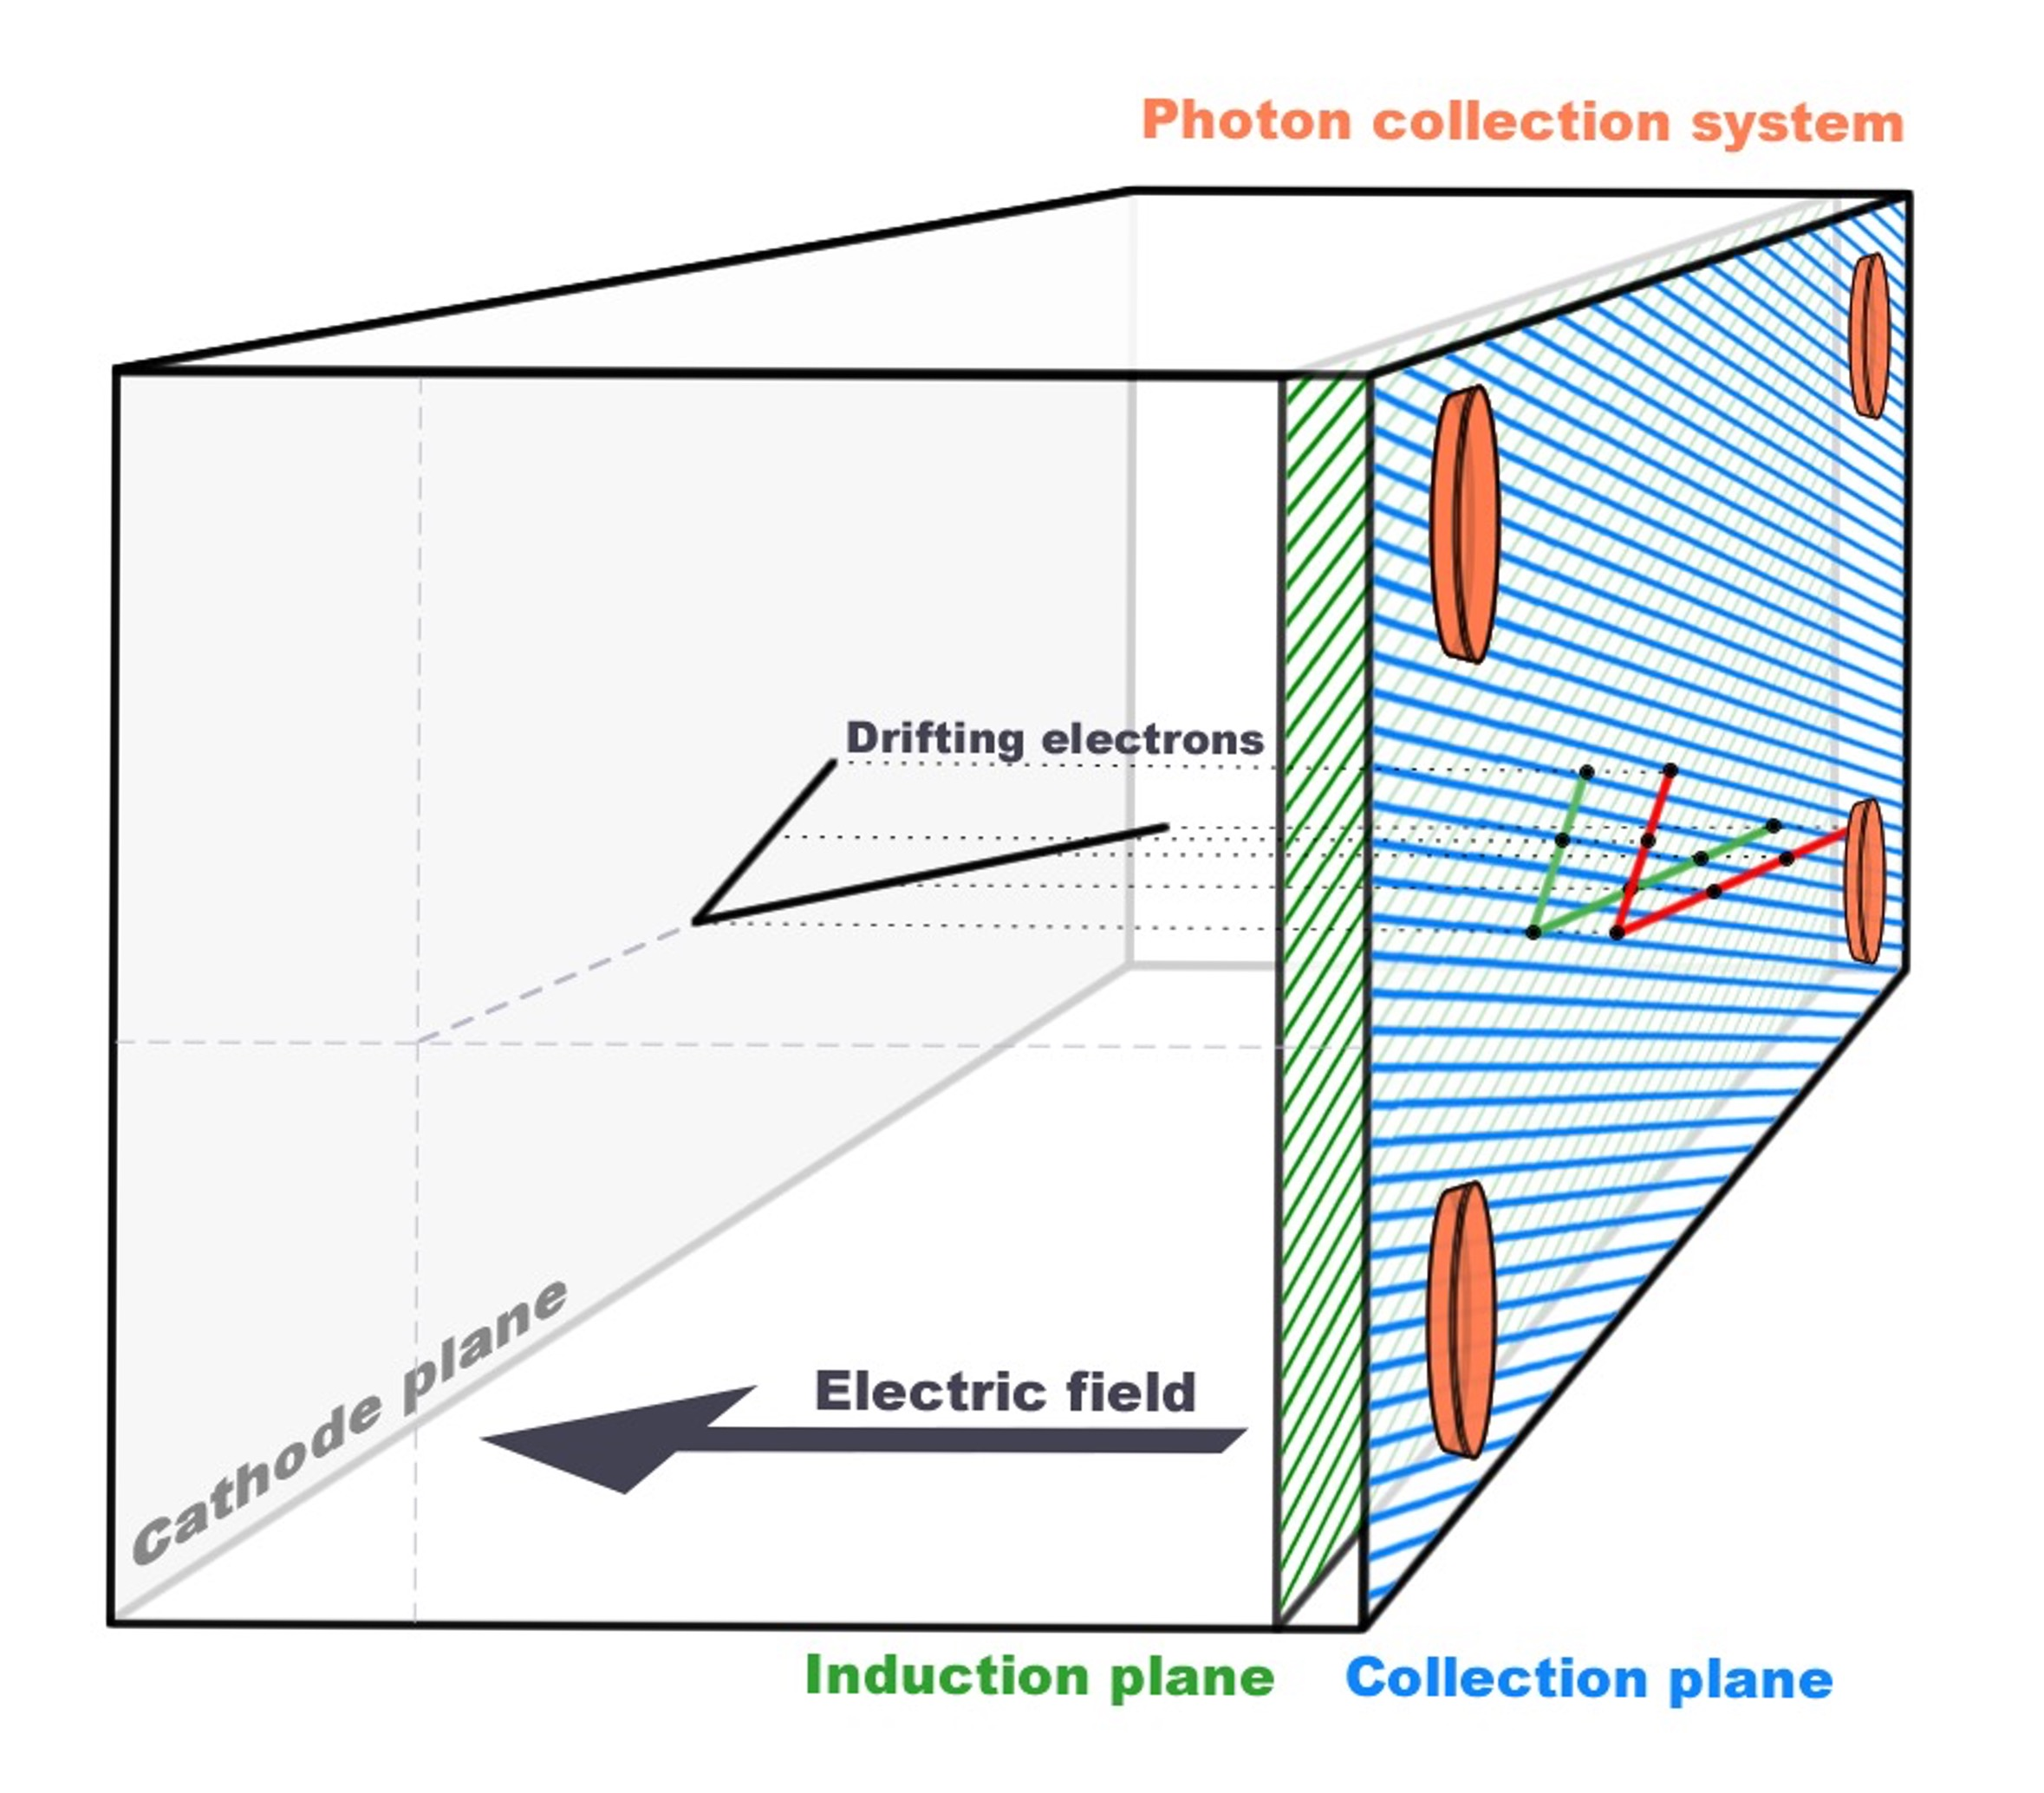
\includegraphics[scale=0.1]{Figures/LARTPC.jpg}
		\caption[LArTPC]{ {\textbf{Liquid Argon Time Projection Chamber}} \\ Liquid Argon Time Projection Chamber. When a particle passes through its fiducial volume and interacts with the liquid argon, ionization electrons and scintillation light are produced. The electric field drifts the electrons from where they are produced towards the planes of wires (right corner in the figure). Both charge and light produced are read by precision wires and a light collection system (in the figure, the orange bodies behind the wires), respectively.}
		\label{lartpc}	
	\end{center}
\end{figure}

\begin{figure}
	\begin{center}
		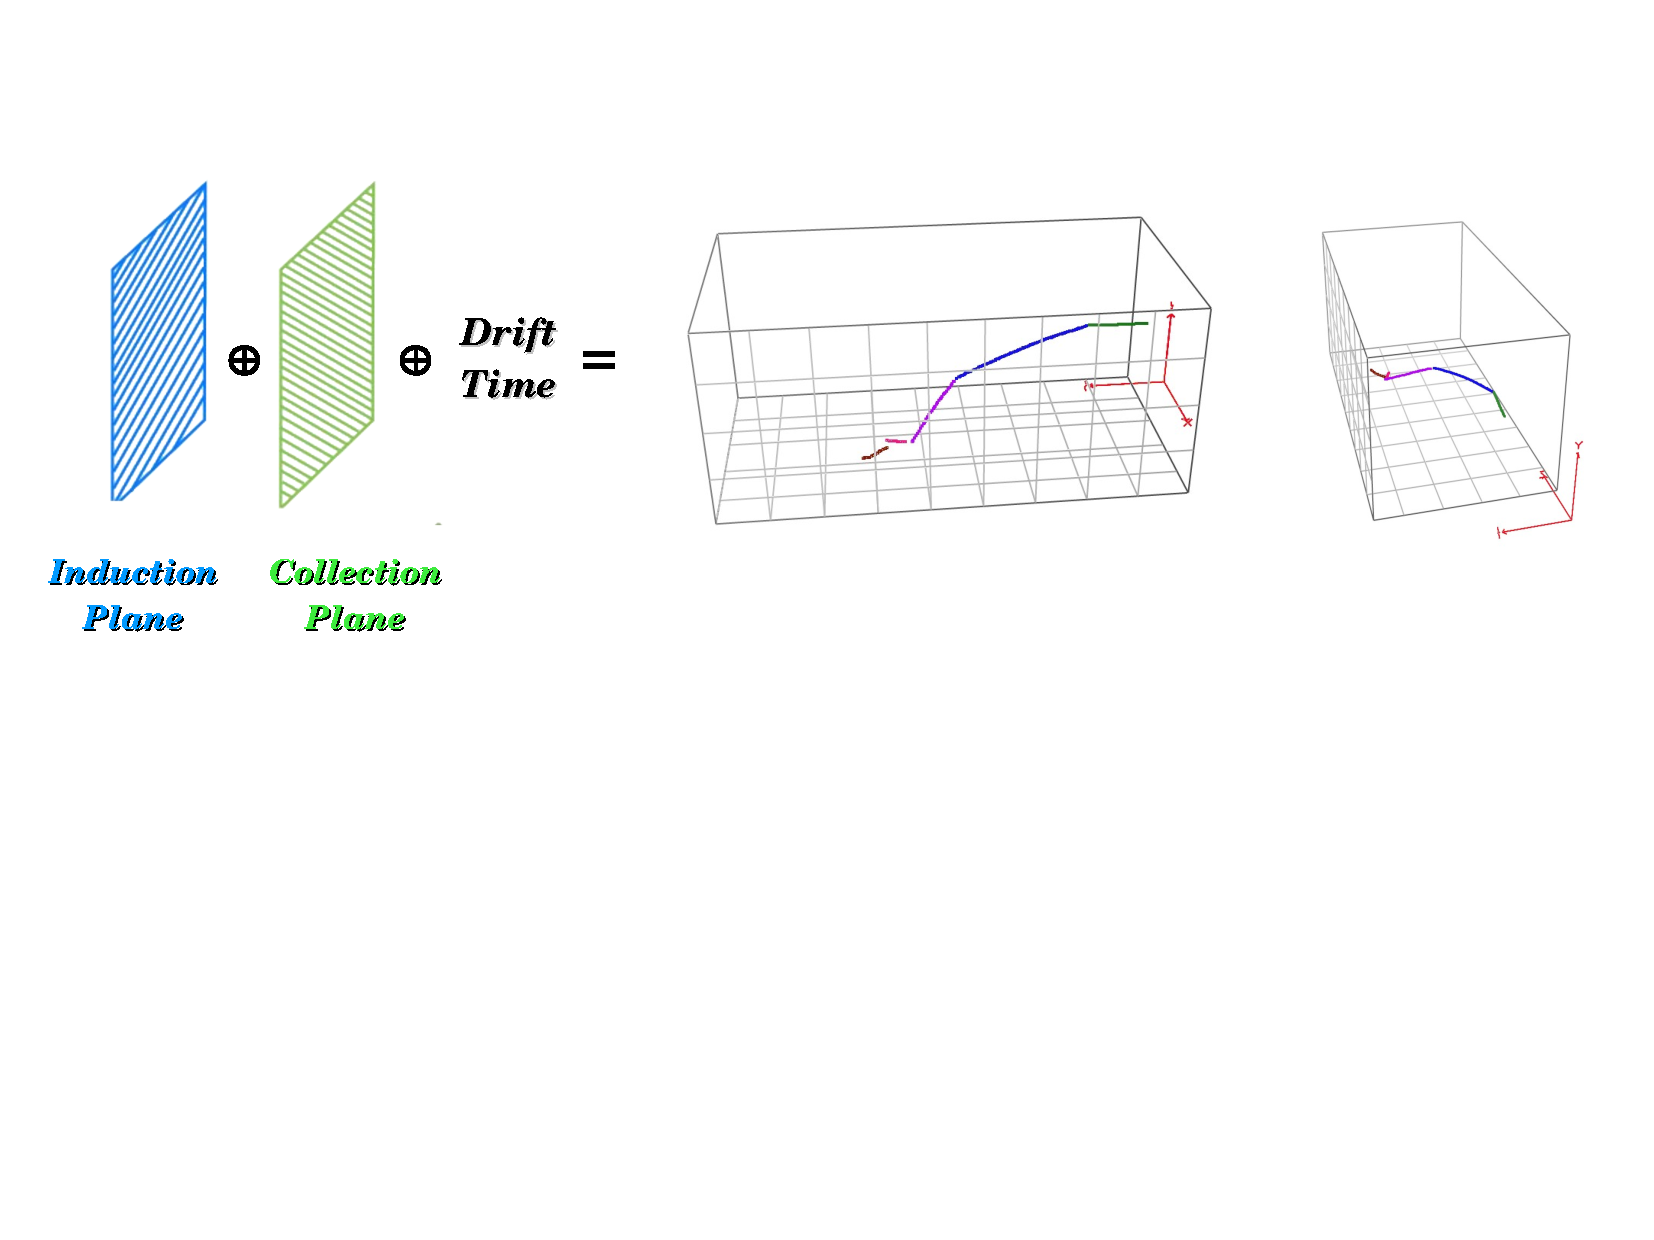
\includegraphics[scale=0.6]{Figures/Acciarri_fig2.pdf}
		\caption[LArTPC read out system]{ {\textbf{LArTPC read out system}} \\ Basic elements of the LArTPC read out system. It is needed a minimum of one induction wire plane, one collection wire plane and a light detection system. The information retrieved by those 3 components allow a 3D track reconstruction \cite{Acciarri_presentation}.}
		\label{lartpc_readout}	
	\end{center}
\end{figure}

\newpage
Not long after, in 1977, Carlo Rubia noted that using Liquid Argon (LAr) as active material in a TPC was particularly advantageous for neutrino physics, since:
\begin{itemize}
	\item it is dense (1.4 g/cm$^3$), which increases the interaction probability;
 	\item it does not attach electrons, allowing long drift distances, which allows the construction of big detectors;
  	\item it has a high electron mobility;
   	\item argon is the third most abundant gas in the atmosphere, it is easy to obtain and purify, making it relatively cheap;
  	\item it is inert and and can be liquified with liquid nitrogen \cite{Rubia_ANewConcept}
\end{itemize}

Ever since, LArTPCs have been the technology of choice of many neutrino physics experiments, such as  Imaging Cosmic and Rare Underground Signals (ICARUS), \cite{ICARUS_proposal}, MicroBooNE, \cite{microboone_proposal}, Short Baseline Neutrino Detector (SBND), \cite{SBND}, that together form the Short Baseline Neutrino (SBN) Program, and Deep Underground Neutrino Experiment (DUNE) \cite{dune_snowmass_22}, to name a few. 

\section{The Short Baseline Neutrino Program}

In a new attempt to get to a conclusion regarding the LEE, described in session, Fermilab created the SBN Program. The program consists of three LArTPCs (SBND, MicroBooNE, and ICARUS) all located along the BNB beam. The principle is that, by having three different detectors of the same technology, exposed to the same beam, and all positioned at a short-baseline range, we will be more accurately be able to constrain our flux of neutrinos and possibly have an answer to the LEE anomalies observed so far, and search for sterile neutrinos. Beyond that, it aims to study neutrino-nucleus scattering at the GeV energy scale and further develop LArTPC's construction and installation procedures, \cite{SBN}.

Originally, ICARUS was, the first large-scale LArTPC to be used to further our understanding of neutrinos and was located underground at the The Gran Sasso National Laboratory and exposed to the CERN Neutrinos to Gran Sasso (CNGS) beamline \cite{ICARUS_proposal}. Most recently one of its modules, the T600, was refurbished, upgraded and has its new home at Fermilab, in the BNB beam. ICARUS T600 LArTPC is used as the far detector in the SBN Program. It is a $476$ton active mass LArTPC and it seats $600$ m from the target. 

\begin{figure}[h!]
	\begin{center}
		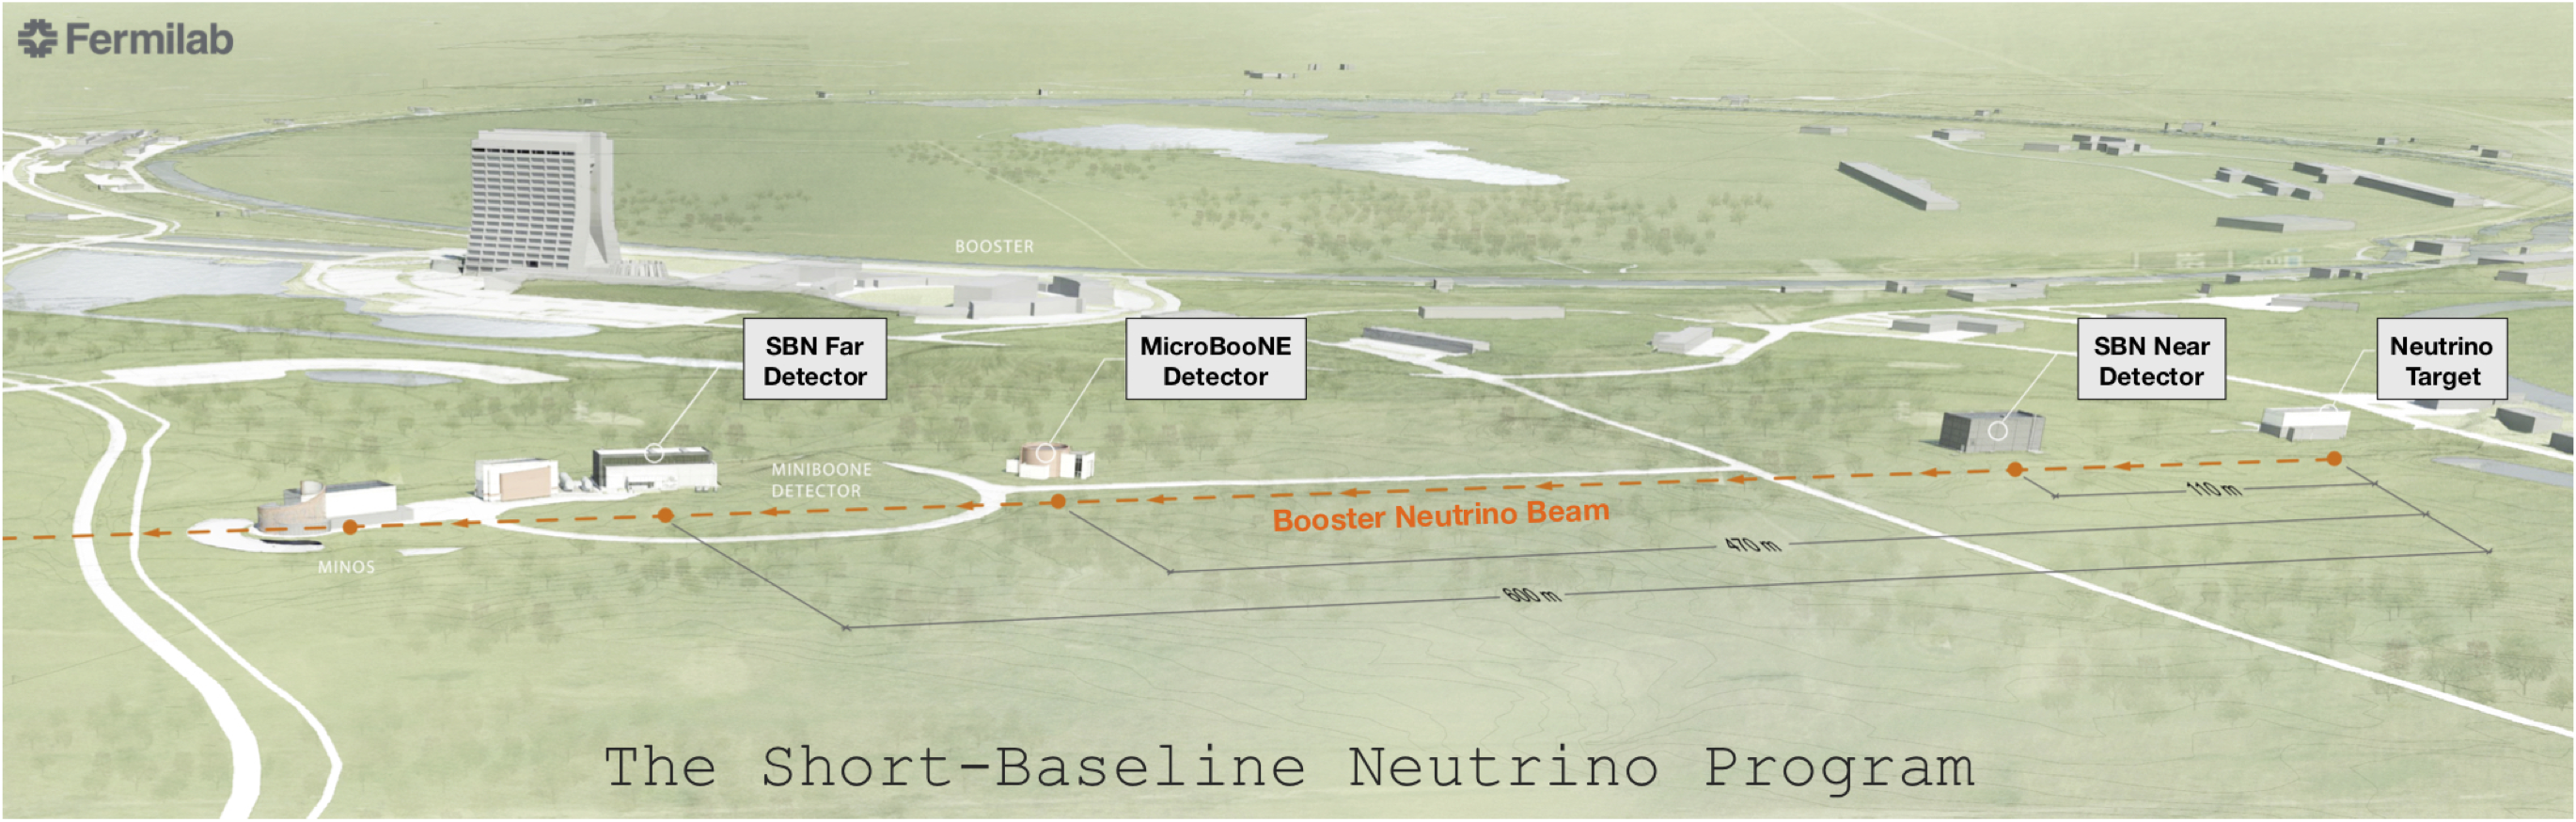
\includegraphics[scale=0.35]{Figures/SBN.png}
		\caption[SBN Program]{The Short-Baseline Neutrino Program detectors as seen from an upper view at Fermilab. To the right is the neutrino beam target area where 8 GeV protons from the Booster accelerator impinge a beryllium target. The beam is focused along the orange dashed line traveling toward the left (north). The SBND, MicroBooNE, and ICARUS, \cite{SBN}.
		}
		\label{sbn_program}
	\end{center}
\end{figure}

The SBND is, as the name implies, the program's near detector and it consists of a $112$ton active mass LArTPC is at $110$ m from the target. It is currently under  installation phase and it is expected to be taking date mid-late next year,2023. In-between ICARUS and SBND, at $470$ m from the target, there is MicroBooNE, a $89$ton active volume LArTPC that has been taking da since 2015. Where each of the detectors are in the BNB beamline, at Fermilab, is illustrated in figure \ref{sbn_program}.
I will later describe in more details SBND and MicroBooNE, as they are the experiments in which I've carried my Ph.D. work. 

\section{The Deep Underground Neutrino Experiment}

The Deep Underground Neutrino Experiment (DUNE) is by far the most promising experiment for neutrino physics, as it aims to measure the CP violating phase in the leptonic sector, to determine the character of the neutrino mass spectrum, and to make precision measurements of oscillation parameters. Beyond the neutrino physics goals, DUNE also aims to search for baryon number violating processes and to perform precision measurements of neutrinos from a core-collapse supernova within the Galaxy, if one happens during the experiment's operating period. 
To accomplish such bold goals, DUNE counts with a near detector placed at Fermilab and a far detector at the Sanford Underground Research Laboratory in Lead, South Dakota. An intense neutrino beam of up to $2.4$ megawatts is produced at Fermilab, crosses the near detector, and travels $1,300$ kilometers downstream through Earth's crust to reach the far detector. In figure \ref{DUNE_full_schematic} you can see an schematic diagram of the experiment. 

\begin{figure}[h!]
	\begin{center}
		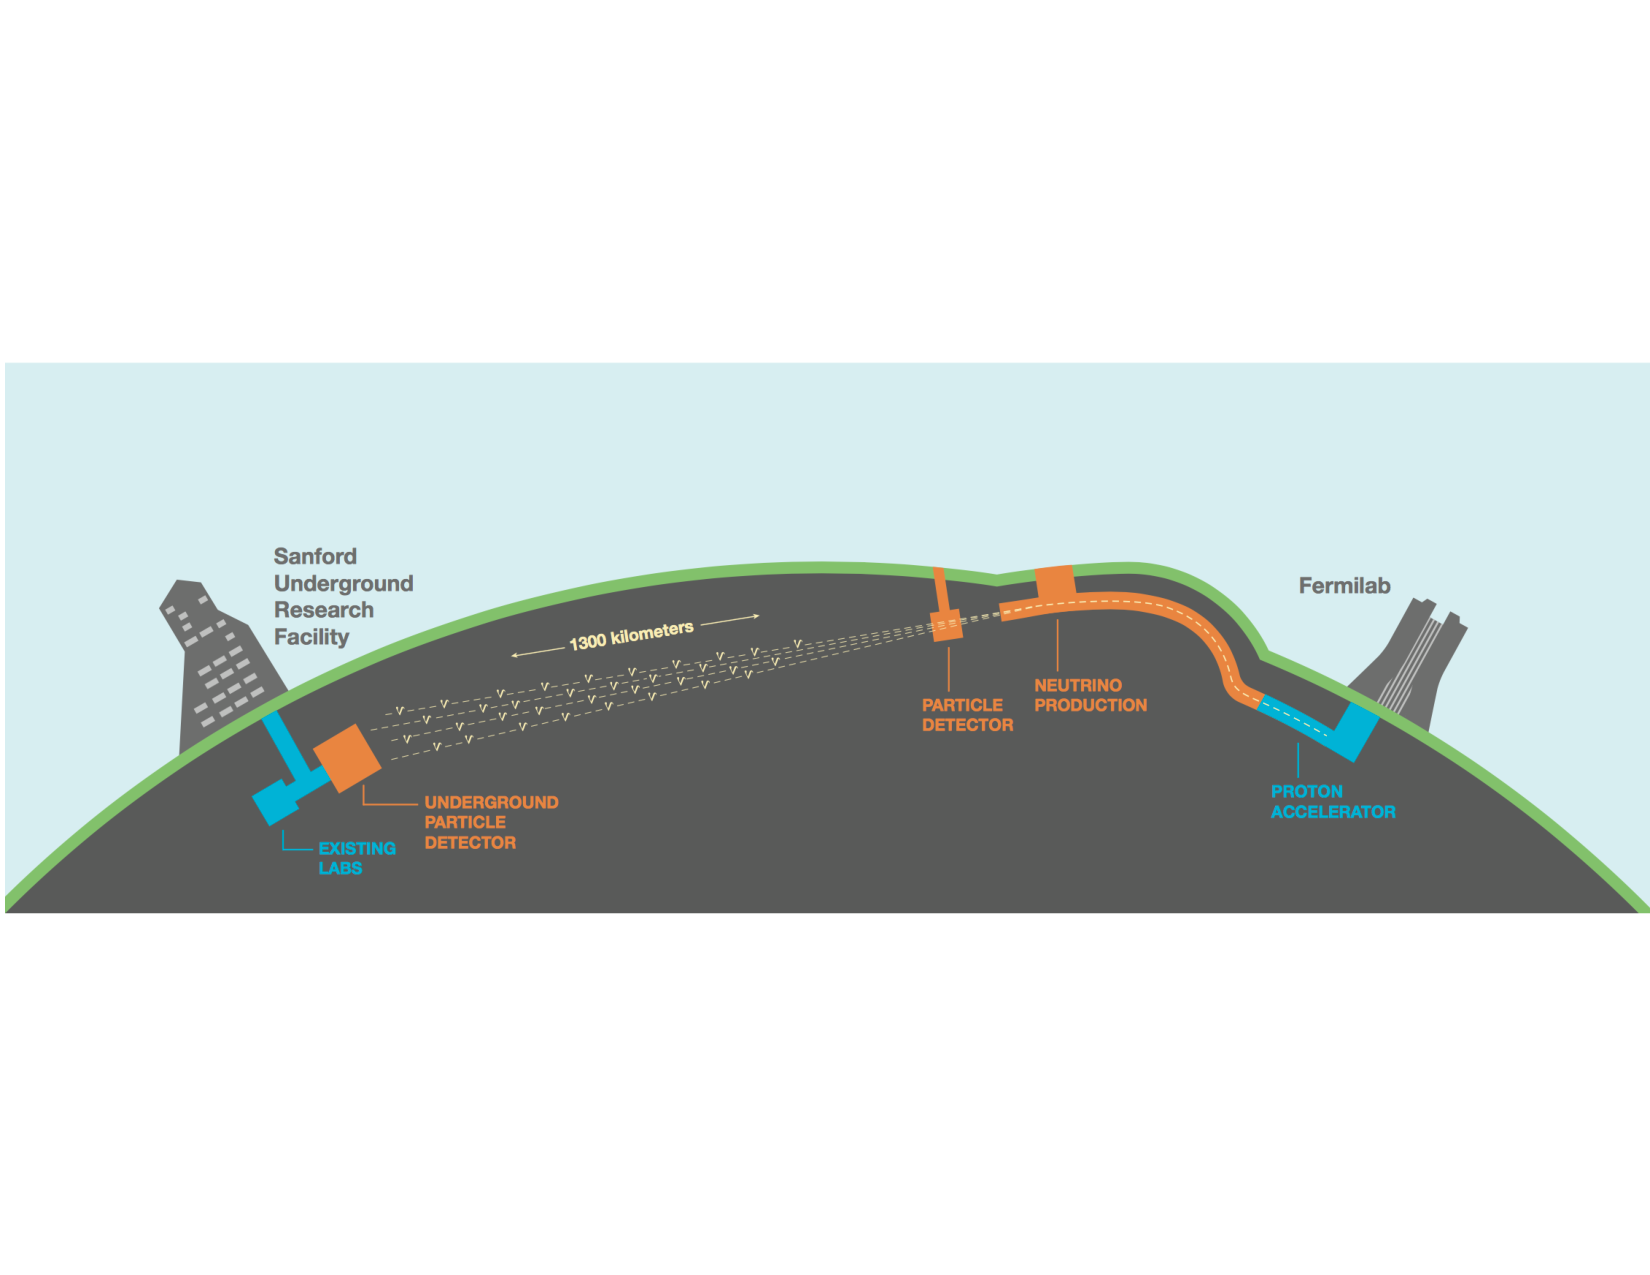
\includegraphics[scale=0.6]{Figures/DUNE_full_schematic.pdf}
		\caption[DUNE's full schematic]{ {\textbf{DUNE's full schematic.}} \\The figure shows the full DUNE's schematics, providing a view of the production of the neutrino beam, the Near Detector at Fermilab, the under crust travel of the beam, and the Far Detector at SURF \cite{dune_snowmass_22}.}
		\label{DUNE_full_schematic}	
	\end{center}
\end{figure}

DUNE's far detector is made of $4$ LArTPCs modules, of $10$ kton each. The near detector will have a combination of three different detection systems: a modular and optically segmented LArTPC of $\approx300$ tons (ND-LAr), a magnetized high-pressure Gas Argon Time Projection Chamber (GArTPC) surrounded by a calorimeterm (ND-GAr), a magnetized beam monitor consisting of an electromagnetic calorimeter, an inner target/tracker system and an active LAr target (SAND). \cite{dune_snowmass_22, dune_SAND}.

\chapter{Liquid Argon Time Projection Chambers in Neutrino Physics}
\section{Overview of the MicroBooNE Experiment}
The MicroBooNE experiment is made of a LArTPC exposed to the neutrino beams at Fermilab: the Booster Neutrino Beam (BNB) and the Neutrino at the Main Injector (NuMI). The LArTPC is located $470$ m on-axis from the BNB target and $679$ m and $3^{\circ}$ off-axis from the NuMI target. MicroBooNE's primary goal is to provide further insight into the low energy anomalies observed by MiniBooNE, mentioned in Chapter \ref{Chapter:1}. Beyond that, it aims to produce neutrino-LAr cross-sections and further develop the LArTPC technology. It took data from 2015 to 2021 and produced dozens of physics results, and dozens more are in the works. 
In this chapter, I will describe MicroBooNE's LArTPC and light collection system, the NuMI beamline, and the data acquisition and processing. I will not go into details about the BNB beamline as it escapes the scope of this work.

\section{The Detector}

In this session I will brifly describe the MicroBooNE's detector, that has two main components: The LArTPC and the light collection system. 
\subsection{Time Projection Projection Chamber}
As extensively explained in Chapter \ref{Chapter:1}, LArTPCs are very powerful detectors for neutrino physics. They allow tracking reconstruction with precision calorimetric information and event displays that resemble bubble-chamber ones. MicroBooNE's LArTPC is $10.4$ m long along the BNB beam direction, $2.56$ m wide in the drift direction, and $2.33$ m tall. This volume accommodates $87$ ton of liquid argon, which we call the detector's active volume.  

MicroBooNE LArTPC has $3$ planes of wires, $2$ of which are called "induction planes" and produce a bipolar signal when electrons pass through them. One induction wire plane has the wire oriented on $+60^{\circ}$ angle with the vertical, and the other $-60^{\circ}$ angle with the vertical. The third is the collection plane, oriented vertically, which will collect the electrons, producing a unipolar signal, \cite{microboone_electronics}. The $3$ wire planes together form a structure called anode plane assembly (APA). 

\begin{figure}[h!]
	\begin{center}
		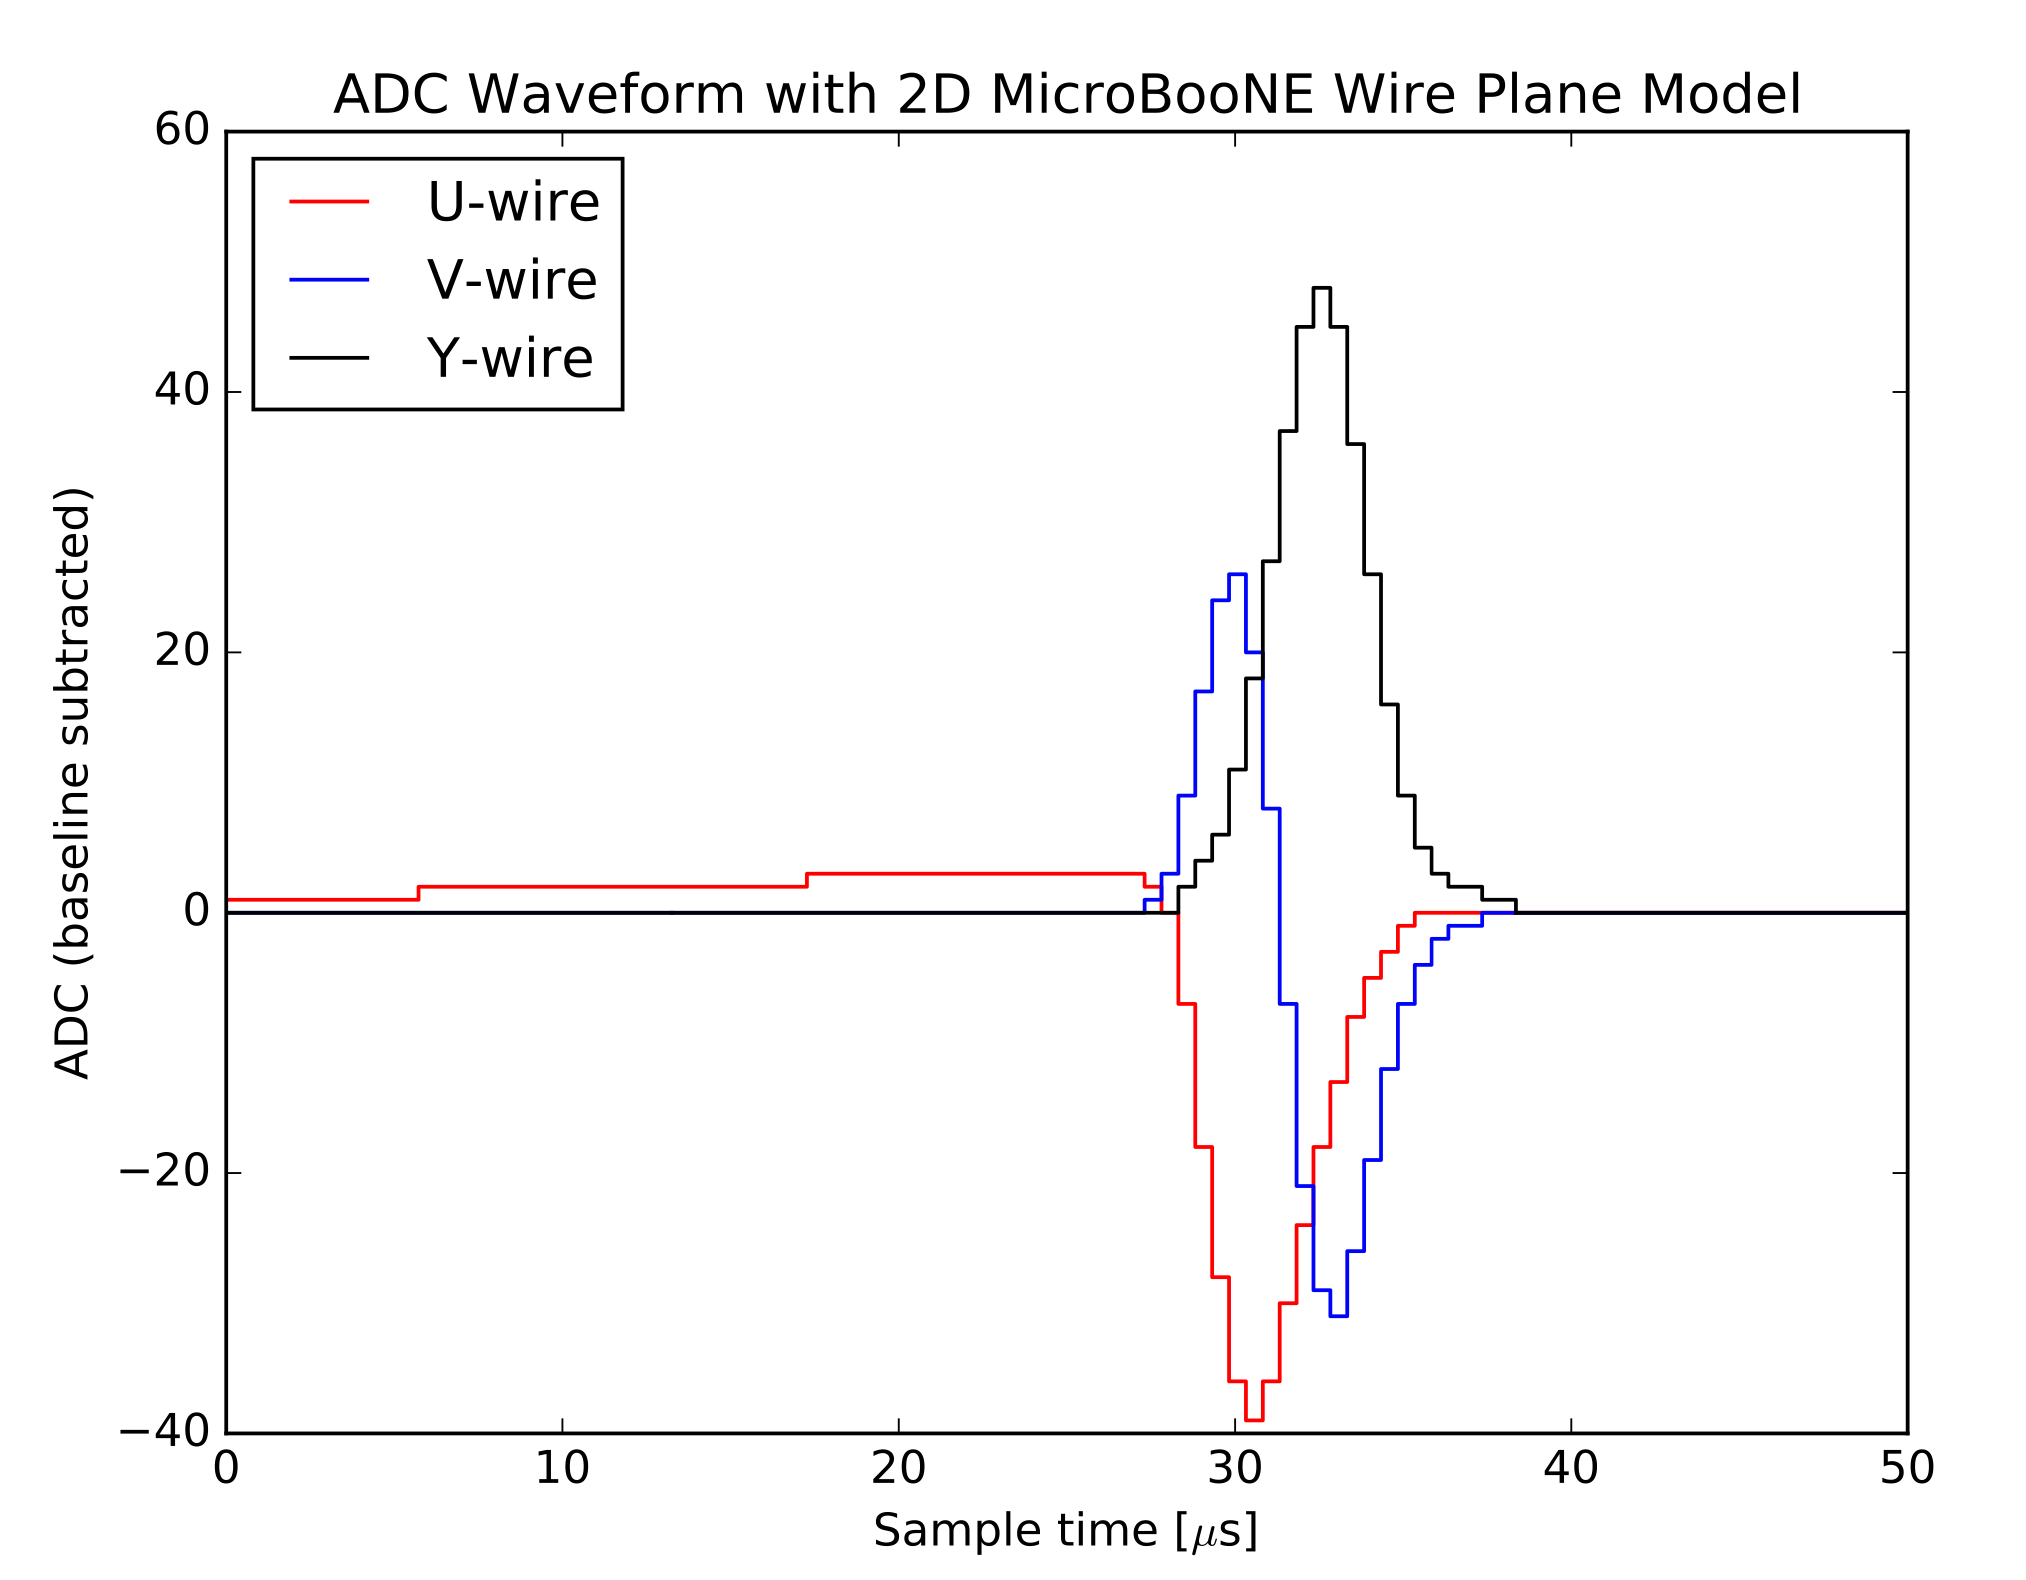
\includegraphics[scale=0.25]{Figures/uboone_dig_signal.png}
		\caption[MicroBooNE's wire planes digital signal]{{\textbf{MicroBooNE's wire planes digital signal}}  \\ Simulation of the digitalized signal of MicroBooNE's wire planes. The U plane corresponds to the induction at $+60^{\circ}$, and the V planes corresponds to the inductin plane at $-60^{\circ}$ and its signal produce takes a bipolar waveform. The Y is the collection plane and its signal takes a unipolar waveform, \cite{microboone_electronics}}
		\label{uboone_digital_signal}	
	\end{center}
\end{figure}

A picture of MicroBooNE's LArTPC assembled can be seen in figure \ref{uboone_lartpc} All three planes have a wire spacing of $3$ mm. The cathode of the LArTPC is at $-70$ V, and the APA is at ground, creating an electric field along the drift direction of $273$ V/cm. At total, MicroBooNE's LArTPC has $8,256$ wires, \cite{microboone_design}. 

\begin{figure}[h!]
	\begin{center}
		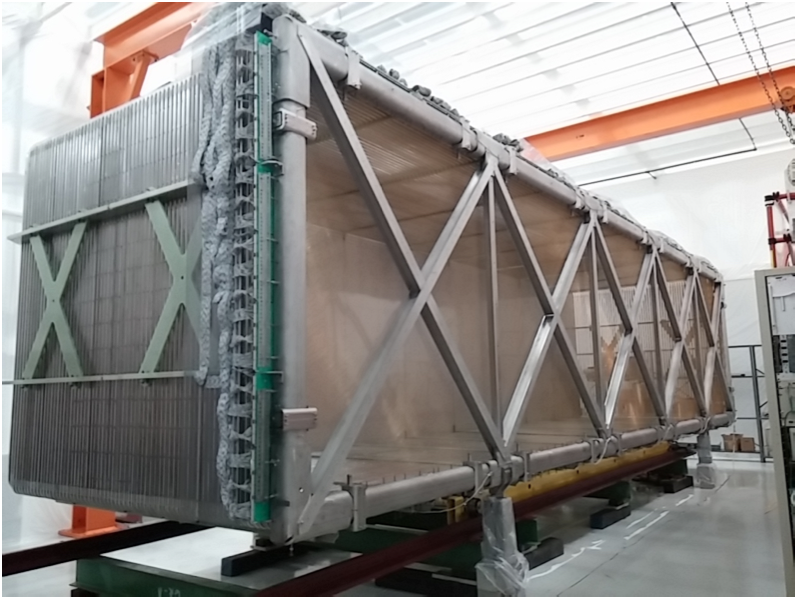
\includegraphics[scale=0.6]{Figures/uboone_LArTPC.png}
		\caption[MicroBooNE's Liquid Argon Time Projection Chamber]{{\textbf{MicroBooNE's Liquid Argon Time Projection Chamber}} \\MicroBooNE's Liquid Argon Time Projection Chamber. The right face is the anode planes face, with the outermost wire plane being the collection plane. \cite{microboone_design}}
		\label{uboone_lartpc}	
	\end{center}
\end{figure}

To keep the argon in liquid form, the LArTPC is immersed in a vessel, called cryostat, that accommodates a total of $170$ ton of Liquid Argon, keeping the temperature at $89$ K and the pressure at $1.2$ atm. How the LArTPC seats inside teh cryostat can be seen in figure \ref{uboone_cryo}.

\begin{figure}[h!]
    \begin{center}
        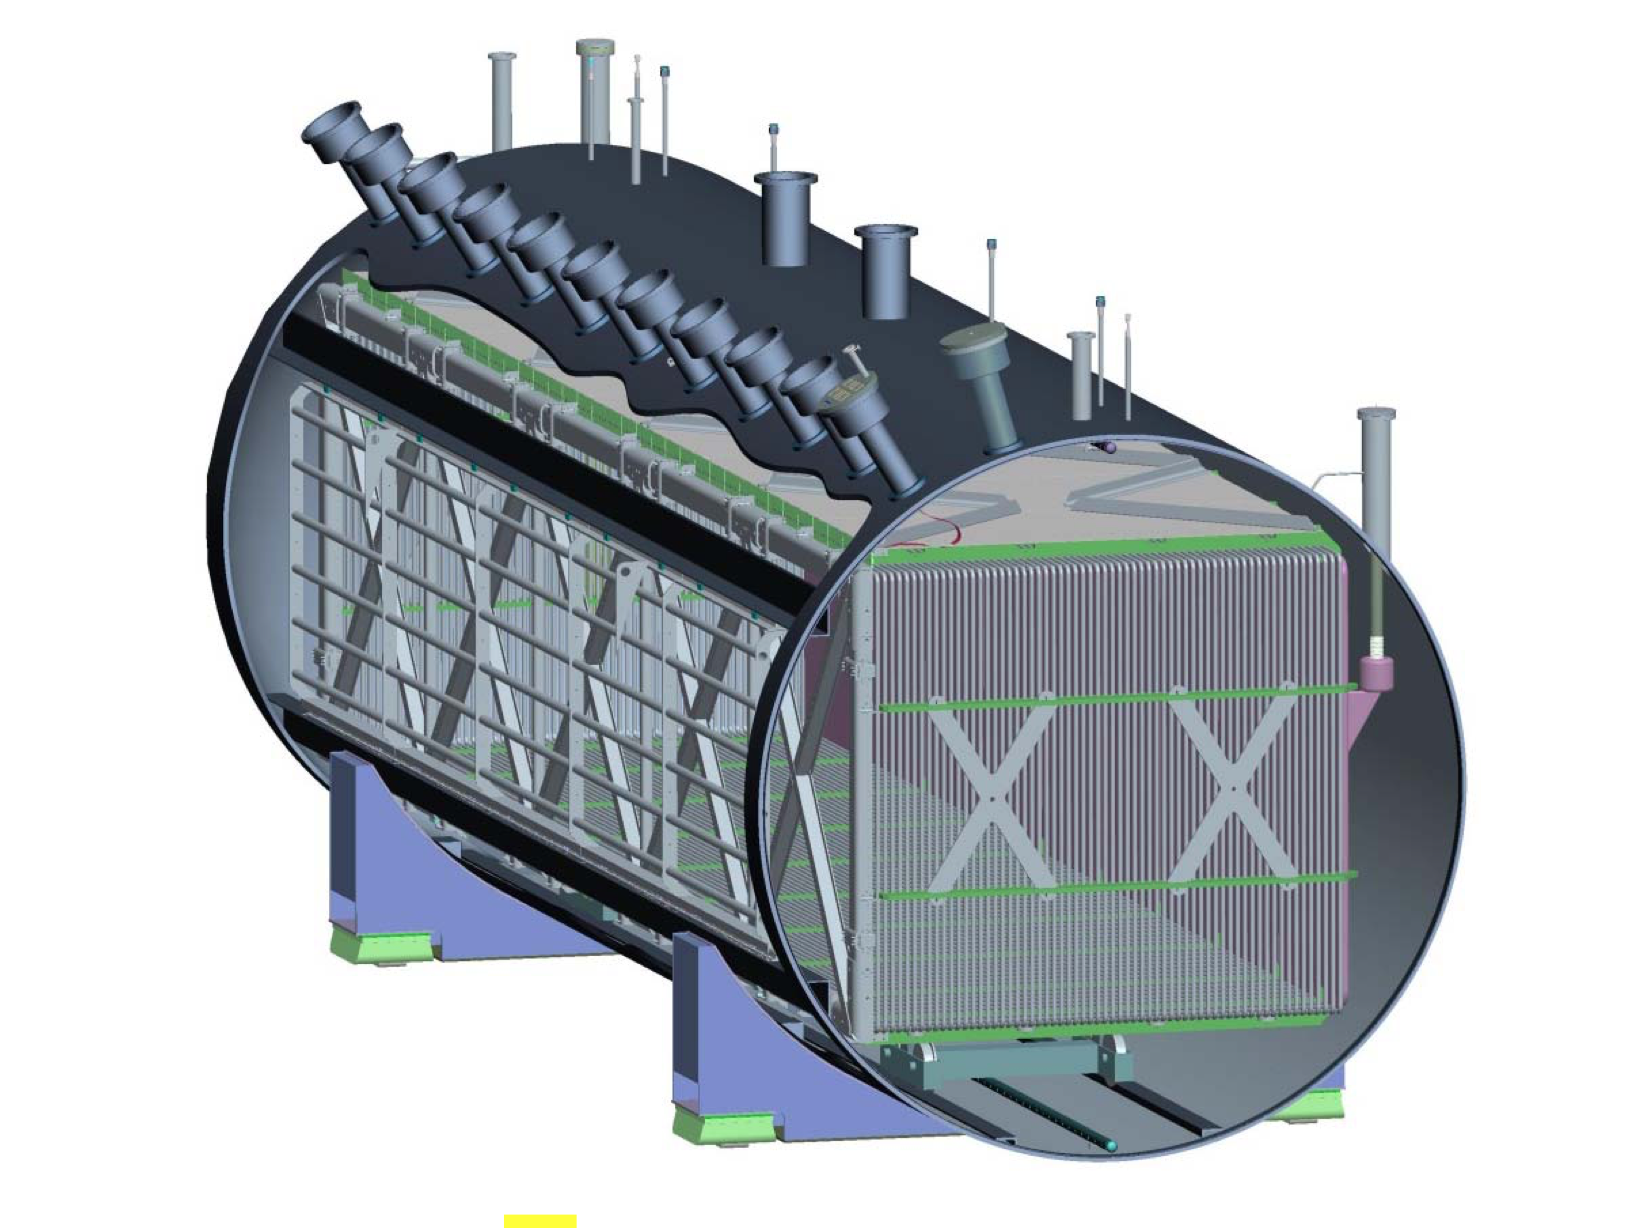
\includegraphics[scale=0.35]{Figures/uboone_cryo.png}
        \caption[MicroBooNE's LArTPC inside the cryostat]{{\textbf{MicroBooNE's LArTPC inside the cryostat}} \\ Schematic view of MicroBooNE's LArTPC inside of the cryostat vessel. The cryostat is the cylindric-like structure in the figure, \cite{microboone_design}.}
        \label{uboone_cryo} 
    \end{center}
\end{figure}

\subsection{Light Collection System}

As mentioned in chapter \ref{Chapter:1}, the scintillation light produced by a charged particle crossing the LArTPC gives the information about the start time of the event. From the difference between the time that the electrons are collected in the collection plane and the start time of the event, plus the knowledge of the drift velocity of the electrons in the detector, we recover the third dimension of the track reconstruction. In MicroBooNE, the drift velocity of the electrons is $1.14$ m/ms. 

This is only possible due to the fact that LAr produces plenty of scintillation light ($\approx 10^4 $) /MeV and that this light is produced and propagated in LAr almost instantaneously ($\approx ns$). The scintillation light is produced in LAr by two mechanisms: self-trapped excitation luminescence and recombination luminescence. Figure \ref{lar-excimers} is a diagram demonstrating those two processes. When a charge particle passes through the liquid argon, it ionizes or excites it. In the first case it will result in light being produced by self-trapped excitation luminescence, which will produce singlet state in $65\%$ of the cases, and a triplet state in $35\%$ of the cases. In the excitation case, it will result in light being produced by recombination luminescence, which will produce singlet states in half of the cases and triplet states in the other half. In all cases the light signal is supressed by impurities in the LAr. Either process produces light with peak at the $128$ nm wavelength, \cite{lar_excimers}.

\begin{figure}[h!]
    \begin{center}
        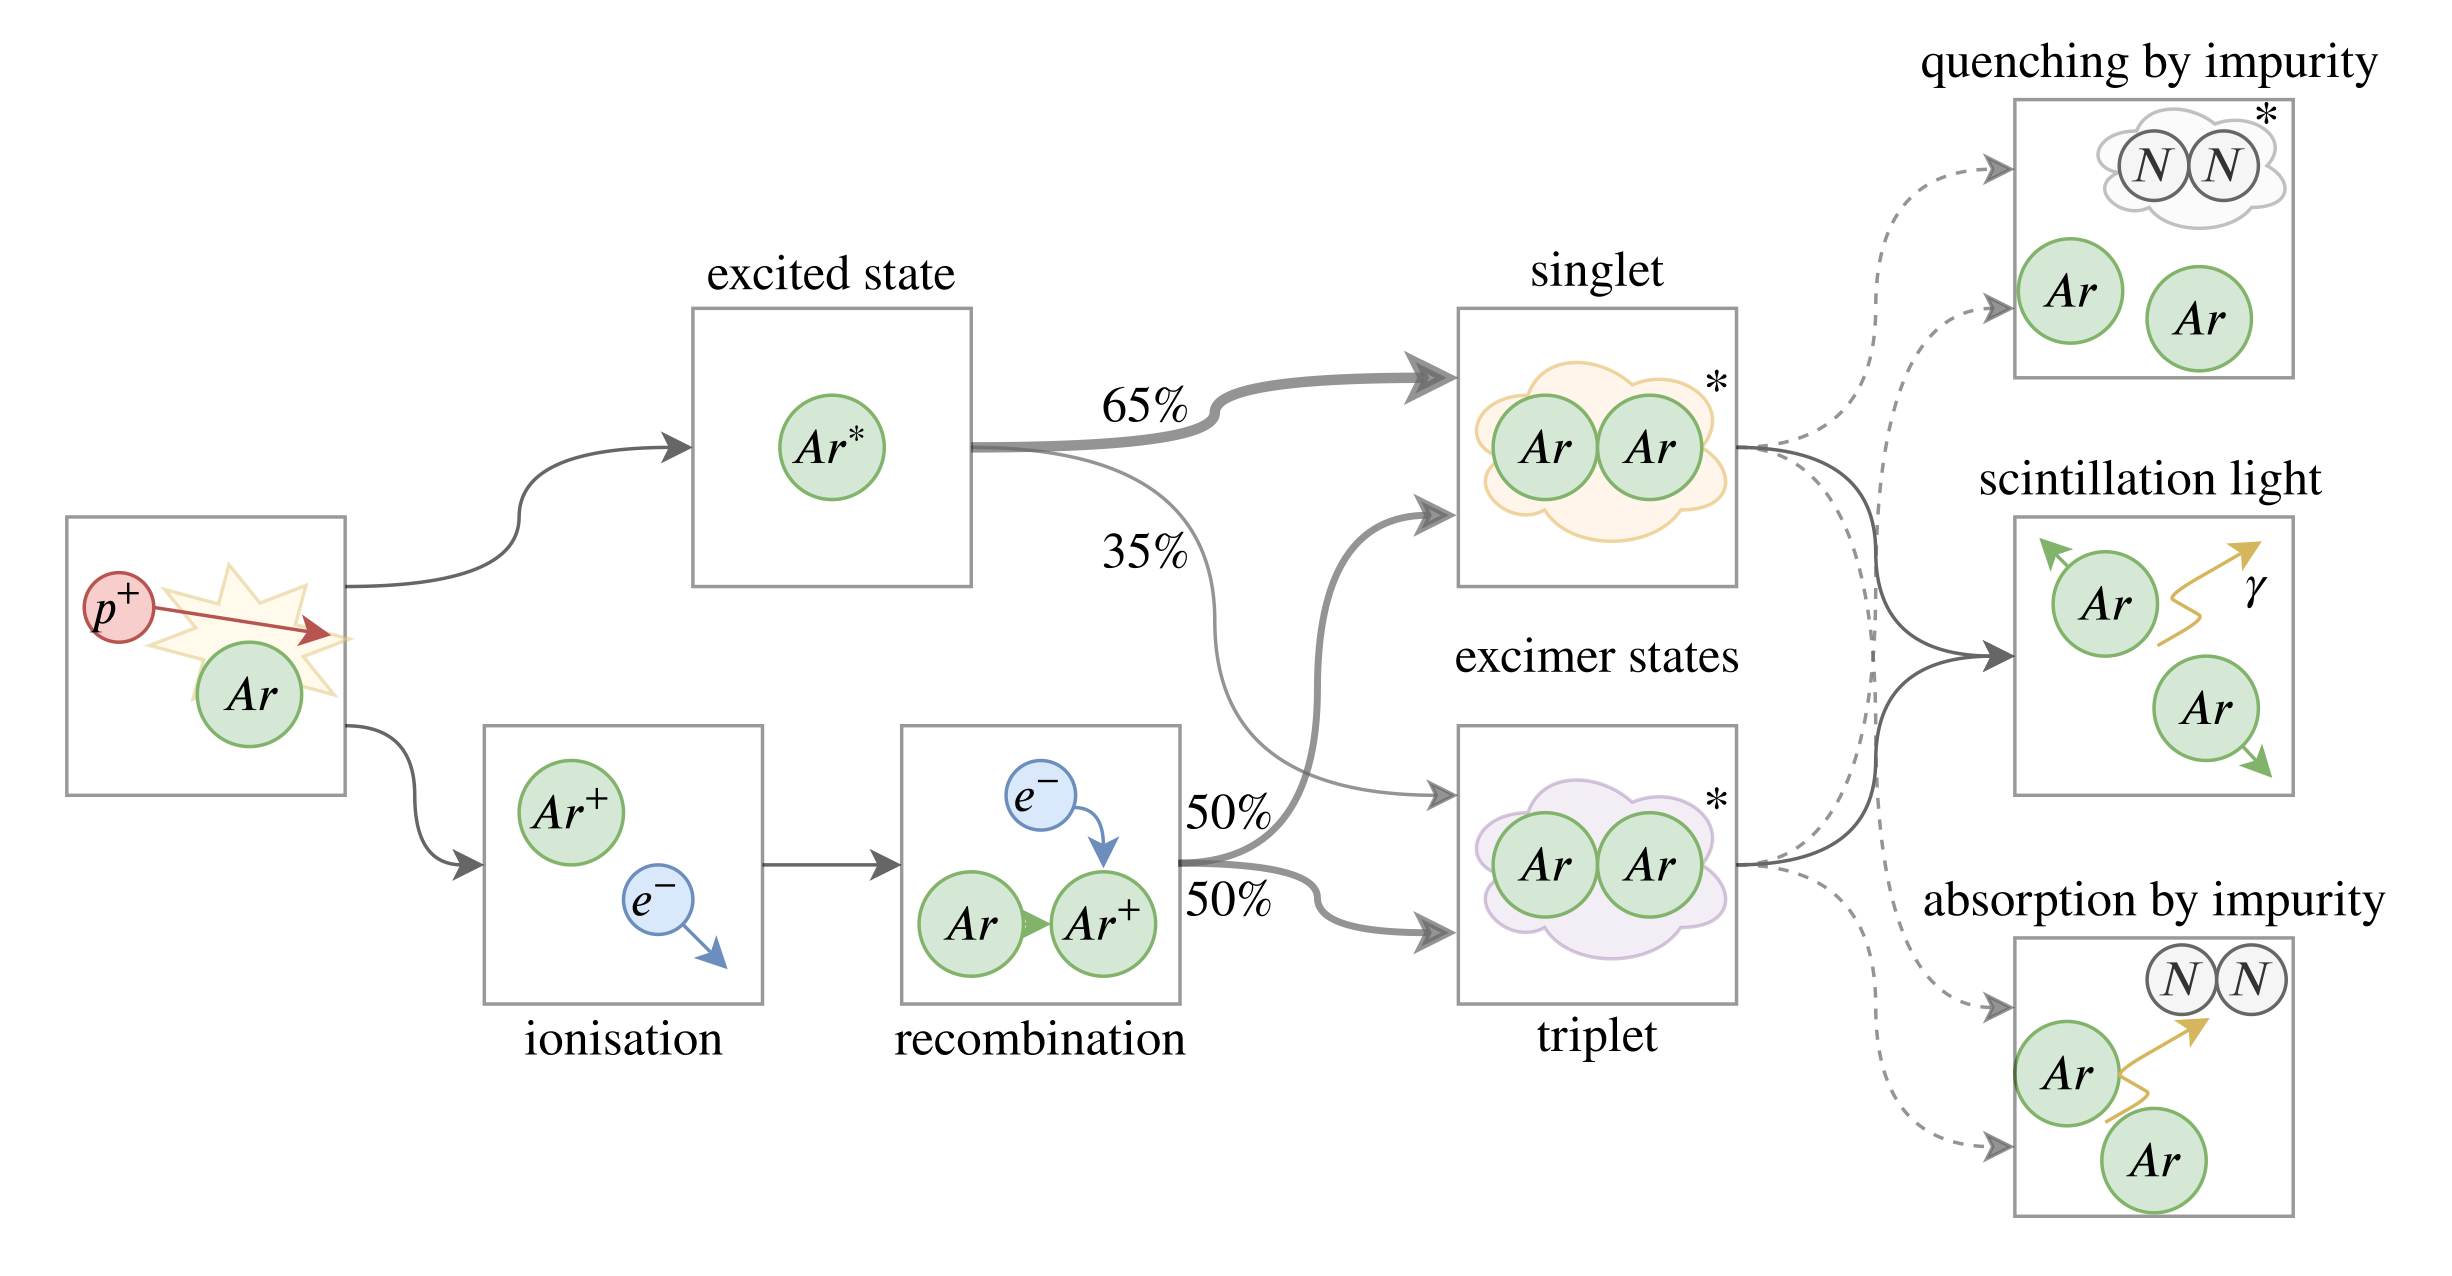
\includegraphics[scale=0.35]{Figures/lar_excimers.png}
        \caption[Scintillation light in liquid argon]{{\textbf{Scintillation light in liquid argon}} When a charge particle passes through the liquid argon, it ionizes or excites it. In the first case it will result in light being produced by self-trapped excitation luminescence In the excitation case, it will result in light being produced by recombination luminescence. In all cases the light signal is supressed by impurities in the LAr. \cite{lar_excimers}.}
        \label{uboone_cryo} 
    \end{center}
\end{figure}

To detect all this light signal, MicroBooNE has $32$ units of 8-inch Hamamatsu photomultiplier tubes (PMTs) arranged behind the APA. Each of them is covered with a plate of tetraphenyl butadiene (TPB) wavelength-shifter, that absorbs the $128$ nm photons and re-emits them at $\approx425$ nm, which is compatible with the PMT's maximum quantum efficiency. A picture of a MicroBooNE PMT is in figure \ref{uboone_pmt}.

\begin{figure}[h!]
    \begin{center}
        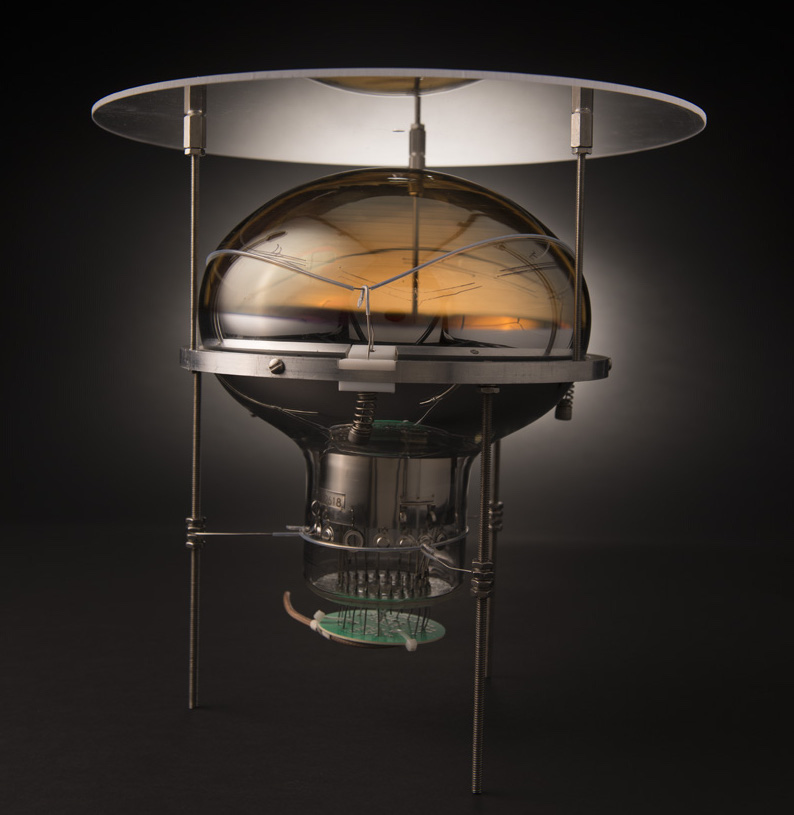
\includegraphics[scale=0.2]{Figures/microboone_pmt.jpeg}
        \caption[MicroBooNE's PMT]{{\textbf{MicroBooNE's PMT}} From: \cite{uboone_pmt}.}
        \label{uboone_pmt} 
    \end{center}
\end{figure}

\section{Neutrino at the Main Injector (NuMI) Beamline}

To study neutrinos, Fermilab artificially produces neutrinos through an accelerator chain that delivers two beams, the Booster Neutrino Beam (BNB) and the Neutrino at the Main Injector (NuMI) beam. Both supply neutrinos to a variety of experiments. MicroBooNE's main beam is the BNB,  but it is also exposed to the NuMI beam. 

The accelerator chain (see full Fermilab's beam chain in \ref{accelerator_chain}) starts with an ion source machine with a molybdenum cathode installed inside of it and filled with hydrogen gas. The molybdenum's electrons are excited and then collected by the hydrogen atoms. The result is a H$^-$ gas. An "extractor" attracts the negative atoms with a positive potential, pulling them through a hole with a width of a few mm, while a magnetic field guides them in the right direction to feed the beam into a radio-frequency quadrupole (RFQ). The RFQ receives the low-energy beam from the ion source at one end and injects a $750$ keV \cite{RFQ_website} beam into the other end, delivering it to a linear accelerator (LINAC). The LINAC is $150$ m  long and is divided into two acceleration parts. The first is a drift tube that accelerates the beam up to $116$ MeV, and the second is a side-coupled cavity that accelerates the beam up to $401$ MeV \cite{LINAC_website}. Exiting the LINAC, the beam collides with a thin carbon sheet that removes electrons from the H$^-$, resulting in three beams: a $H^-$ beam, a $H^+$ beam, and a $H^0$ beam. Only the pure proton beam is selected. After all this process, the beam is suitable to be inserted into a circular $75$ m radius accelerator called Booster, which extracts a beam of $8$ GeV protons that can be directed towards the Main Injector (MI), the BNB target, or to the Recycler \cite{booster_website}. For the NuMI beam, the protons from the Booster are directed towards a $3319.4$ m circumference synchrotron, called the Main Injector, that further accelerates the protons up to $120$ GeV. Those protons are then directed towards a graphite target, where they collide, producing the NuMI beam.

\newpage
\begin{figure}[h!]
	\begin{center}
		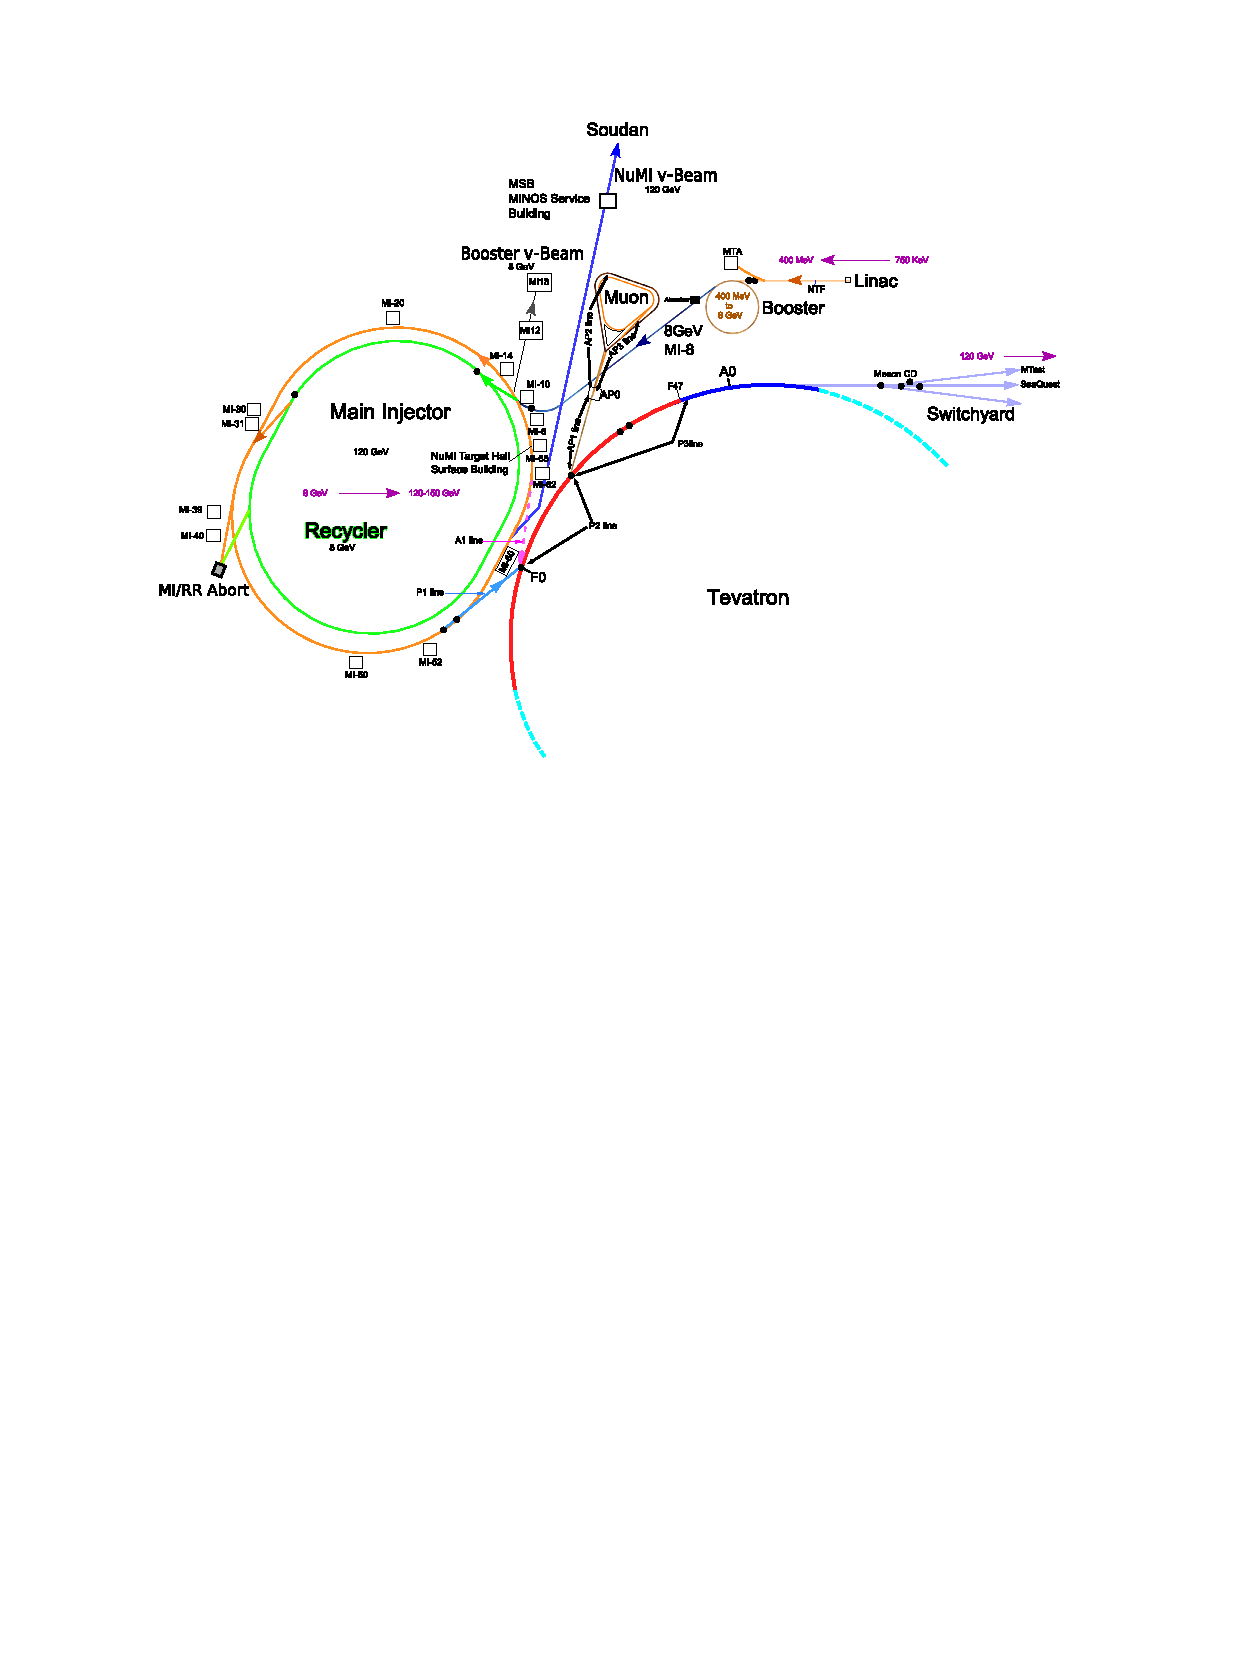
\includegraphics[scale=0.8]{Figures/acceleratorChain.pdf}
		\caption[Full Fermilab's beam chain]{ {\textbf{Full Fermilab's beam chain}} \\ The image shows the Fermilab beam chain map, from the RFQ/LINAC to the main injector, BNB, or to the recycler, \cite{paper_numibeamline}.}
		\label{accelerator_chain}	
	\end{center}
\end{figure}
%

In the NuMI beam, when the $120$ GeV protons are thrown at a graphite target, they produce mesons. These mesons are focused by magnetic horns and directed to the $675$ m long decay pipe, where they decay into muons and muon-neutrinos, as shown in the schematic view of the beamline in figure \ref{fig:numi}. After the decay pipe, an absorber blocks the remaining hadrons and muons in the beamline, leaving a pure neutrino beam beyond it. 

\begin{figure}[h!]
    \centering
    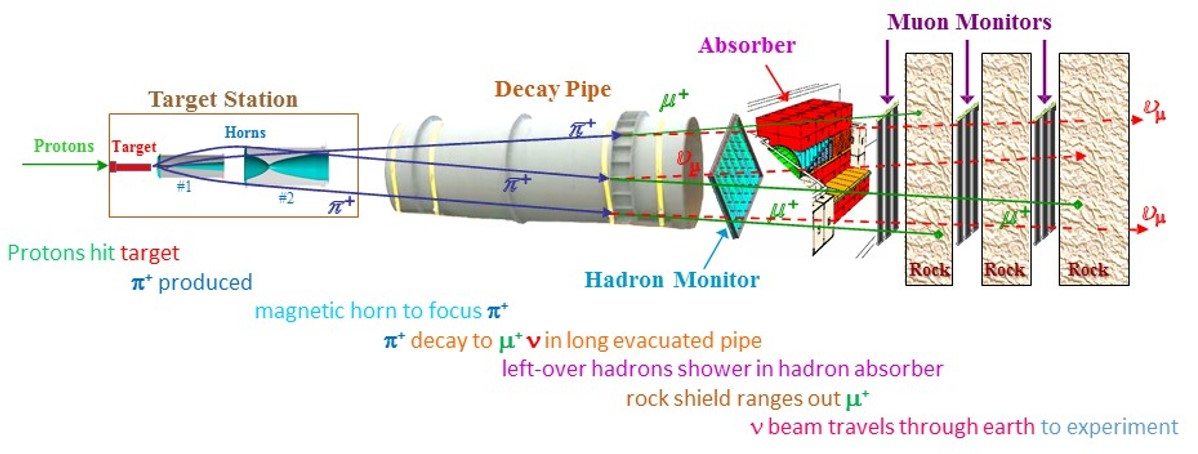
\includegraphics[width=140mm]{Figures/numi.jpg}
    \caption{NuMI layout \cite{numi}.}
    \label{fig:numi}
\end{figure}

By changing the polarity of the magnetic horns, we can select the sign of the charged mesons. By having positive horn current, we select positive particles. We call it the Forward Horn Current (FHC) mode, or Neutrino Mode. By having negative horn current, we select negative particles. We call it the Reverse Horn Current (RHC) mode, or Antineutrino Mode. In figure \ref{beam_mode_uboone} you can find a plot of the number of Protons on Target (POT) delivered in each run of MicroBooNE and in which mode the beam was selected. The NuMI beam delivers neutrinos in windows of $9.6 \mu$ s. During MicroBooNE's operation time we collected a total of $2.3\times 10^{21}$ POT, $1.0\times10^{21}$ in Neutrino Mode and $1.3\times10^{21}$ in Antineutrino Mode

\begin{figure}[h!]
    \centering
    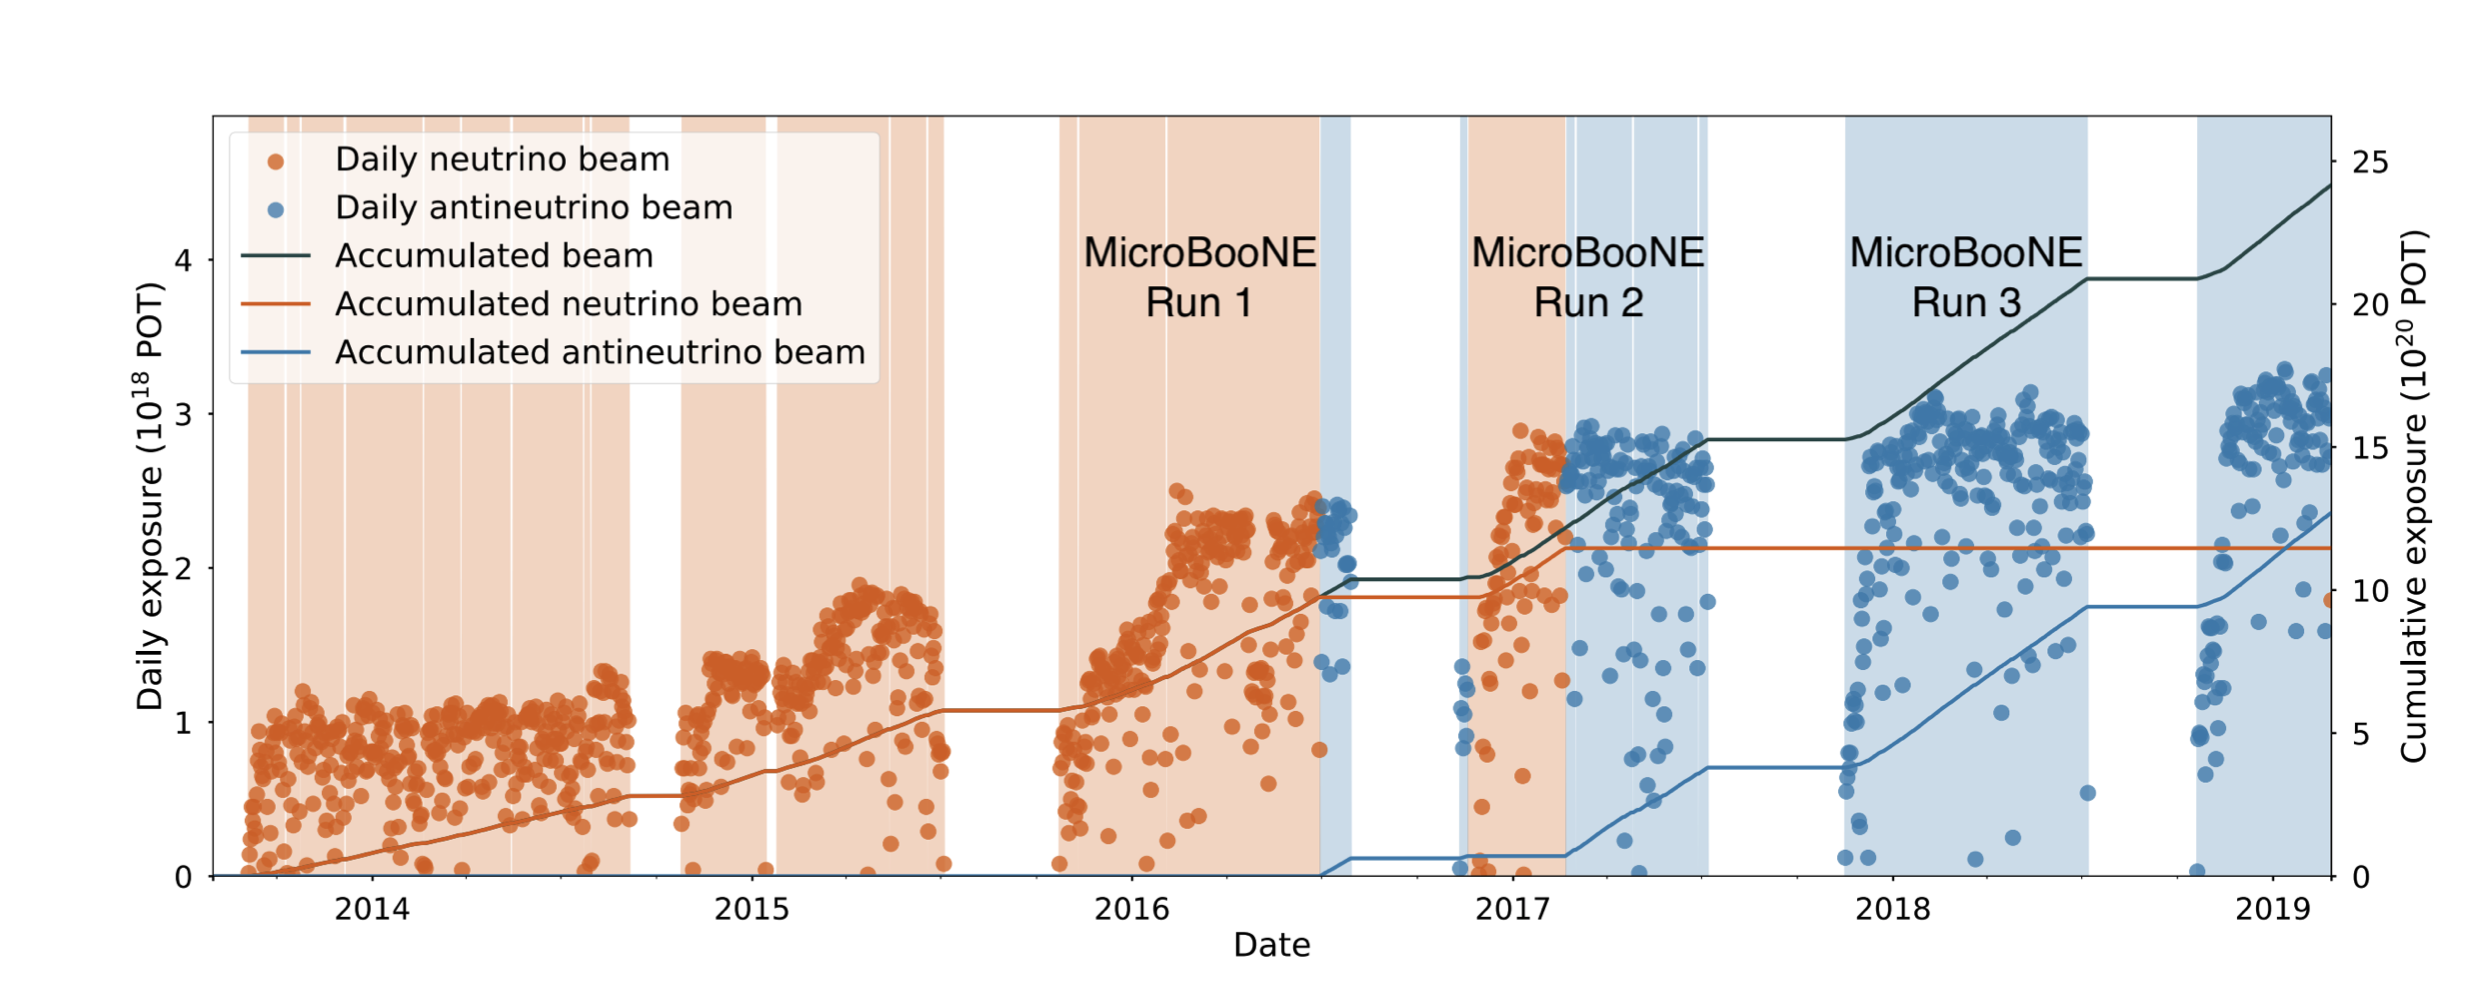
\includegraphics[width=150mm]{Figures/beam_mode_uboone.png}
    \caption{The cumulative POT from NuMI delievered to MicroBrooNE. In the orange regions the horn polarity was in Neutrino Mode. In the blue regions the horn polarity was in Antineutrino Mode. The white regions refer to periods in which the accelerator complex was shut down. \cite{krish_phd}.}
    \label{beam_mode_uboone}
\end{figure}

\section{MicroBooNE's Readout and Trigger Systems}

As a surface detector, MicroBooNE's PMTs and TPC receive particle activities all the time, and recording all this data would be impossible. Additionally, only $2-3\%$ of the pulses of protons sent to the target (called "spills") to produce the neutrinos in the NuMI beam will create a neutrino interaction in MicroBooNE. We use a trigger system to decide what data is recorded.
The trigger system starts with a signal from Fermilab's accelerator complex informing us they sent a new spill. This signal is our hardware (HW) trigger. The HW trigger gives a start to what we call the "beamgate window", in which we start the readout without any light intensity requirement (also known as "unbiased"), which lasts $23.4$ $\mu $s. This happens $1.6$ ms into the TPC readout frame. The NuMI beam spill time window goes from $5.64- 15.44$ $\mu$s into the beamgate window. The complete readout cycle takes 3 TPC readout frames, which takes a total of $4.8$ ms.
The data collected is then passed to a buffer where a software will decide what will be permanently recorded on tape. This is our software (SW) trigger. To be recorded, the SW trigger requires the data to have at least $9.5$ PE of scintillation light in a time window of $4.69- 16.41$ $\mu$s from the beginning of the beamgate window. To account for some decline on the PMT's, during Run 3 the light requirement was updated to $5.75$ PE, \cite{numi_redmine}. 
Around $14\%$ of all HW triggers pass the SW trigger conditions. 

For a visual of the readout and trigger structure, please see the diagram in figure \ref{trig}.

\begin{figure}[h!]
    \centering
    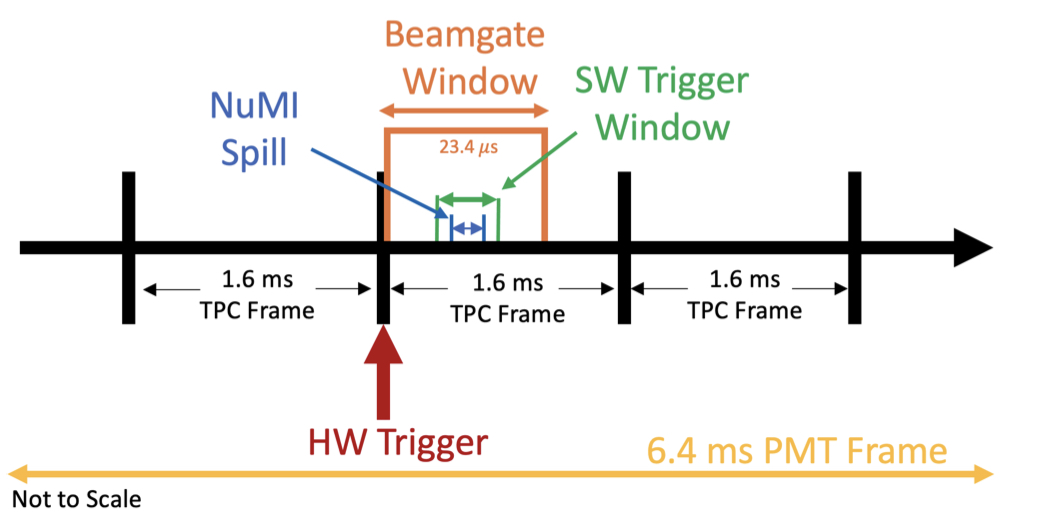
\includegraphics[width=130mm]{Figures/numi_trigger.jpg}
    \caption{Structure of MicroBooNE's NuMI readout and trigger. \cite{krish_phd}.}
    \label{trig}
\end{figure}

From the data collected, MicroBooNE produces three data streams:
\begin{itemize}
    \item NuMI: For this stream, the data has to pass both the hardware and software triggers described above. It is also referred to as "beam-on" data. 
    \item EXT NuMI: This is some data that passes the light requirements of the software trigger but is outside the beamgate window. The light is produced by cosmic rays, and this data is essential for us to understand the background of the neutrino analysis. It is also called "beam-off" data. 
    \item EXT unbiased: This is data that is not in the beamgate window but with no additional requirements. Data from this stream is used to make our simulated events more realistic, as we overlay them with the simulated neutrino interactions. The procedure we use for that is documented in \cite{afro_phd}. 
\end{itemize}

MicroBooNE has a similar data stream, readout and trigger systems for the BNB beam, but with its own time windows. The beamgate window for the BNB and NuMI beams do not overlap. 



\chapter{The MicroBooNE Experiment}
\section{Overview of the MicroBooNE Experiment}
\label{Chapter:2}
The Micro Booster Neutrino Experiment (MicroBooNE) features the first large-scale LArTPC exposed to both the Booster Neutrino Beam (BNB) and Neutrinos at the Main Injector (NuMI) beamlines at Fermilab. The LArTPC is located at $470$ m on-axis from the BNB target and $679$ m and $3^{\circ}$ off-axis from the NuMI target. MicroBooNE's primary goal is to provide further insight into the low energy anomalies observed by MiniBooNE, mentioned in Chapter \ref{Chapter:1}. Beyond that, it aims to measure neutrino-LAr cross-sections and further develop the LArTPC technology. It took data from 2015 to 2021 and produced dozens of physics results; dozens more are in the works. 
In this chapter, I will describe MicroBooNE's LArTPC and light collection system, the NuMI beamline, and the data acquisition and processing. I will not go into details about the BNB beamline as it escapes the scope of this work.

\section{The Detector}

In this section, I will briefly describe the two main components of the MicroBooNE detector: the LArTPC and the light collection system.
\subsection{Time Projection Projection Chamber}
As extensively explained in Chapter \ref{Chapter:1}, LArTPCs are very powerful detectors for neutrino physics. They allow tracking reconstruction with precision calorimetric information and event displays that resemble bubble-chamber ones. MicroBooNE's LArTPC is $10.4$ m long along the BNB beam direction (z-coordinate), $2.56$ m wide in the drift direction (x-coordinate), and $2.33$ m tall (y-coordinate). Referred to as the ``active volume", this corresponds to $87$ tons of liquid argon 

The MicroBooNE LArTPC has $3$ planes of wires, $2$ of which are called ``induction planes" and produce a bipolar signal when electrons pass through them. One induction wire plane (the U plane) has the wire oriented on $+60^{\circ}$ angle with the vertical, and the other (the V plane) $-60^{\circ}$ angle with the vertical. The third is the collection plane (Y plane), oriented vertically, which will collect the electrons, producing a unipolar signal \cite{microboone_electronics}. In figure \ref{uboone_digital_signal} you can see each plane's signal shape. The $3$ wire planes together form a structure called the anode plane assembly (APA). 

\begin{figure}[h!]
	\begin{center}
		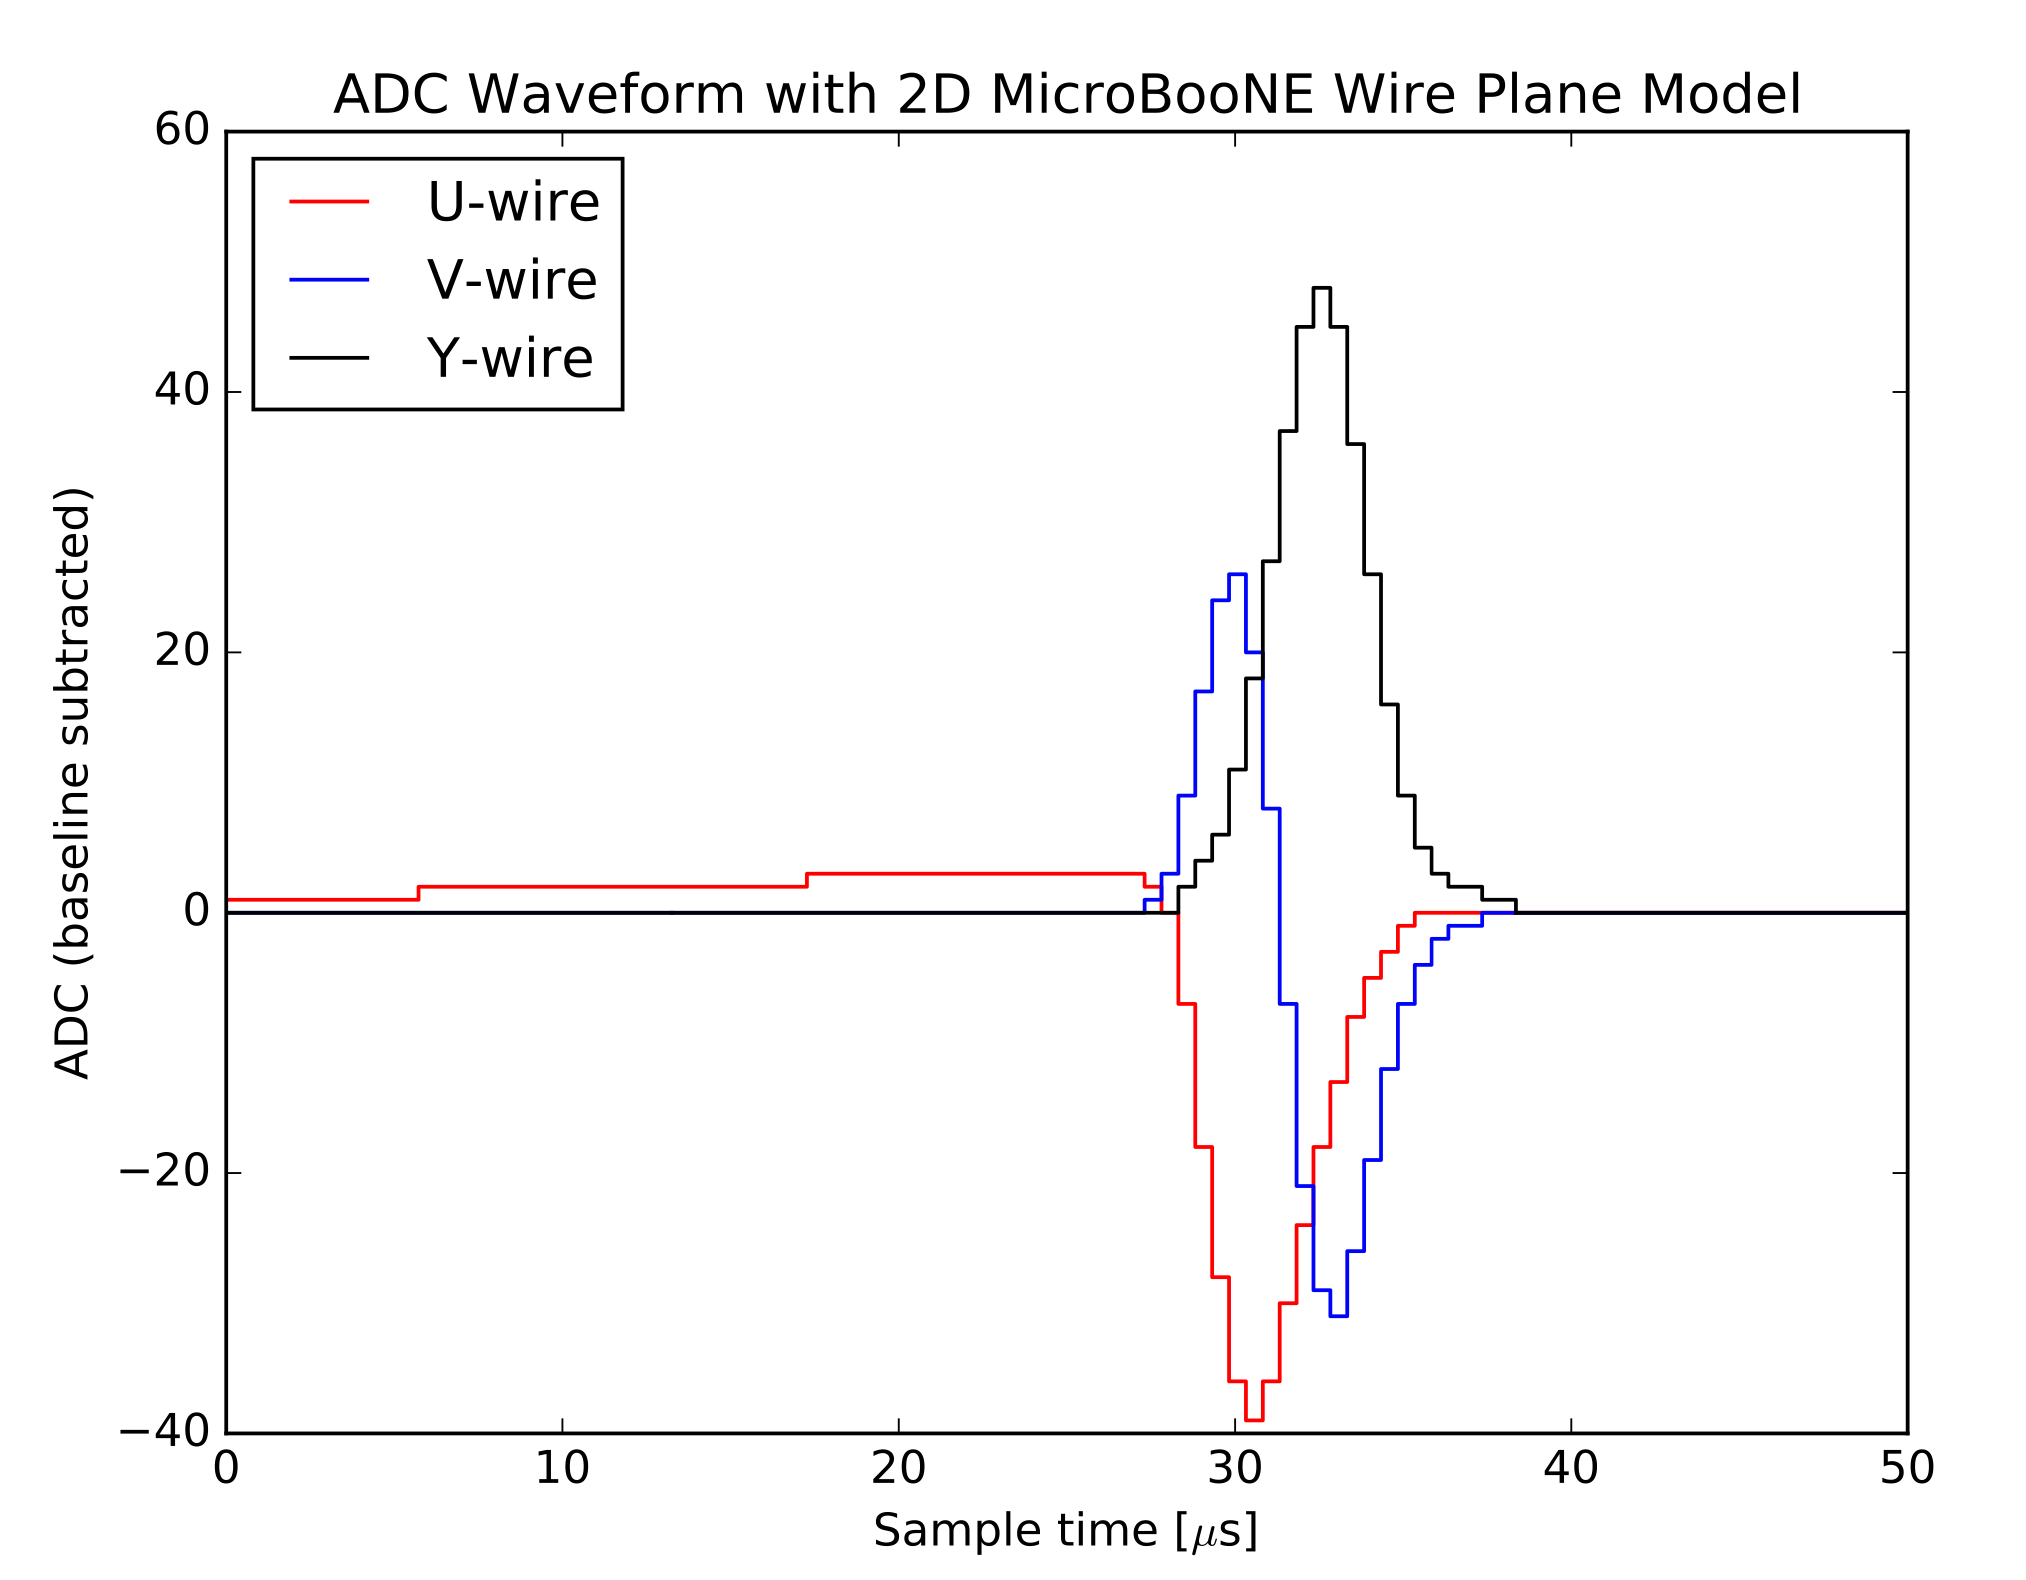
\includegraphics[scale=0.25]{Figures/uboone_dig_signal.png}
		\caption[MicroBooNE's wire planes digital signal]{{\textbf{MicroBooNE's wire planes digital signal}}  \\ The U (V) plane corresponds to the induction wires at $+60$ ($-60$), and induction signals are bipolar in shape. The Y plane corresponds to the vertically-oriented collection wires, whose signals are unipolar in shape.”
        \cite{microboone_electronics}}
		\label{uboone_digital_signal}	
	\end{center}
\end{figure}

A picture of MicroBooNE's assembled LArTPC can be seen in figure \ref{uboone_lartpc} All three planes have a wire spacing of $3$ mm. The cathode of the LArTPC is at $-70$ kV, and the middle induction plane in the APA is at ground, creating an electric field along the drift direction of $273$ V/cm. At total, MicroBooNE's LArTPC has $8,256$ wires \cite{microboone_design}. 

\begin{figure}[h!]
	\begin{center}
		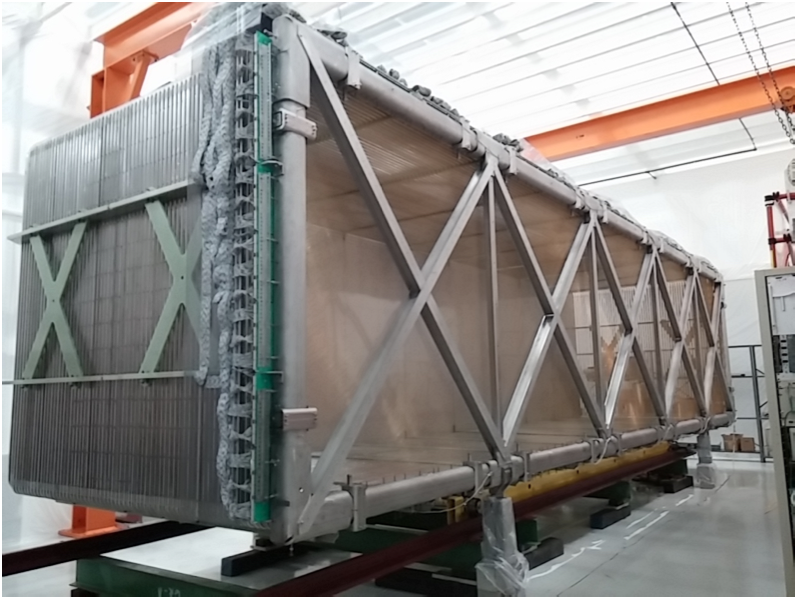
\includegraphics[scale=0.6]{Figures/uboone_LArTPC.png}
		\caption[MicroBooNE's Liquid Argon Time Projection Chamber]{{\textbf{MicroBooNE's Liquid Argon Time Projection Chamber}} \\MicroBooNE's Liquid Argon Time Projection Chamber. The right face is the anode planes face, with the outermost wire plane being the collection plane \cite{microboone_design}.}
		\label{uboone_lartpc}	
	\end{center}
\end{figure}

To keep the argon in liquid form, the LArTPC is immersed in a cryostat, a vessel that accommodates a total of $170$ tons of liquid argon, keeping the temperature at $89$ K and the pressure at $1.2$ atm. How the LArTPC sits inside the cryostat can be seen in figure \ref{uboone_cryo}.

\begin{figure}[h!]
    \begin{center}
        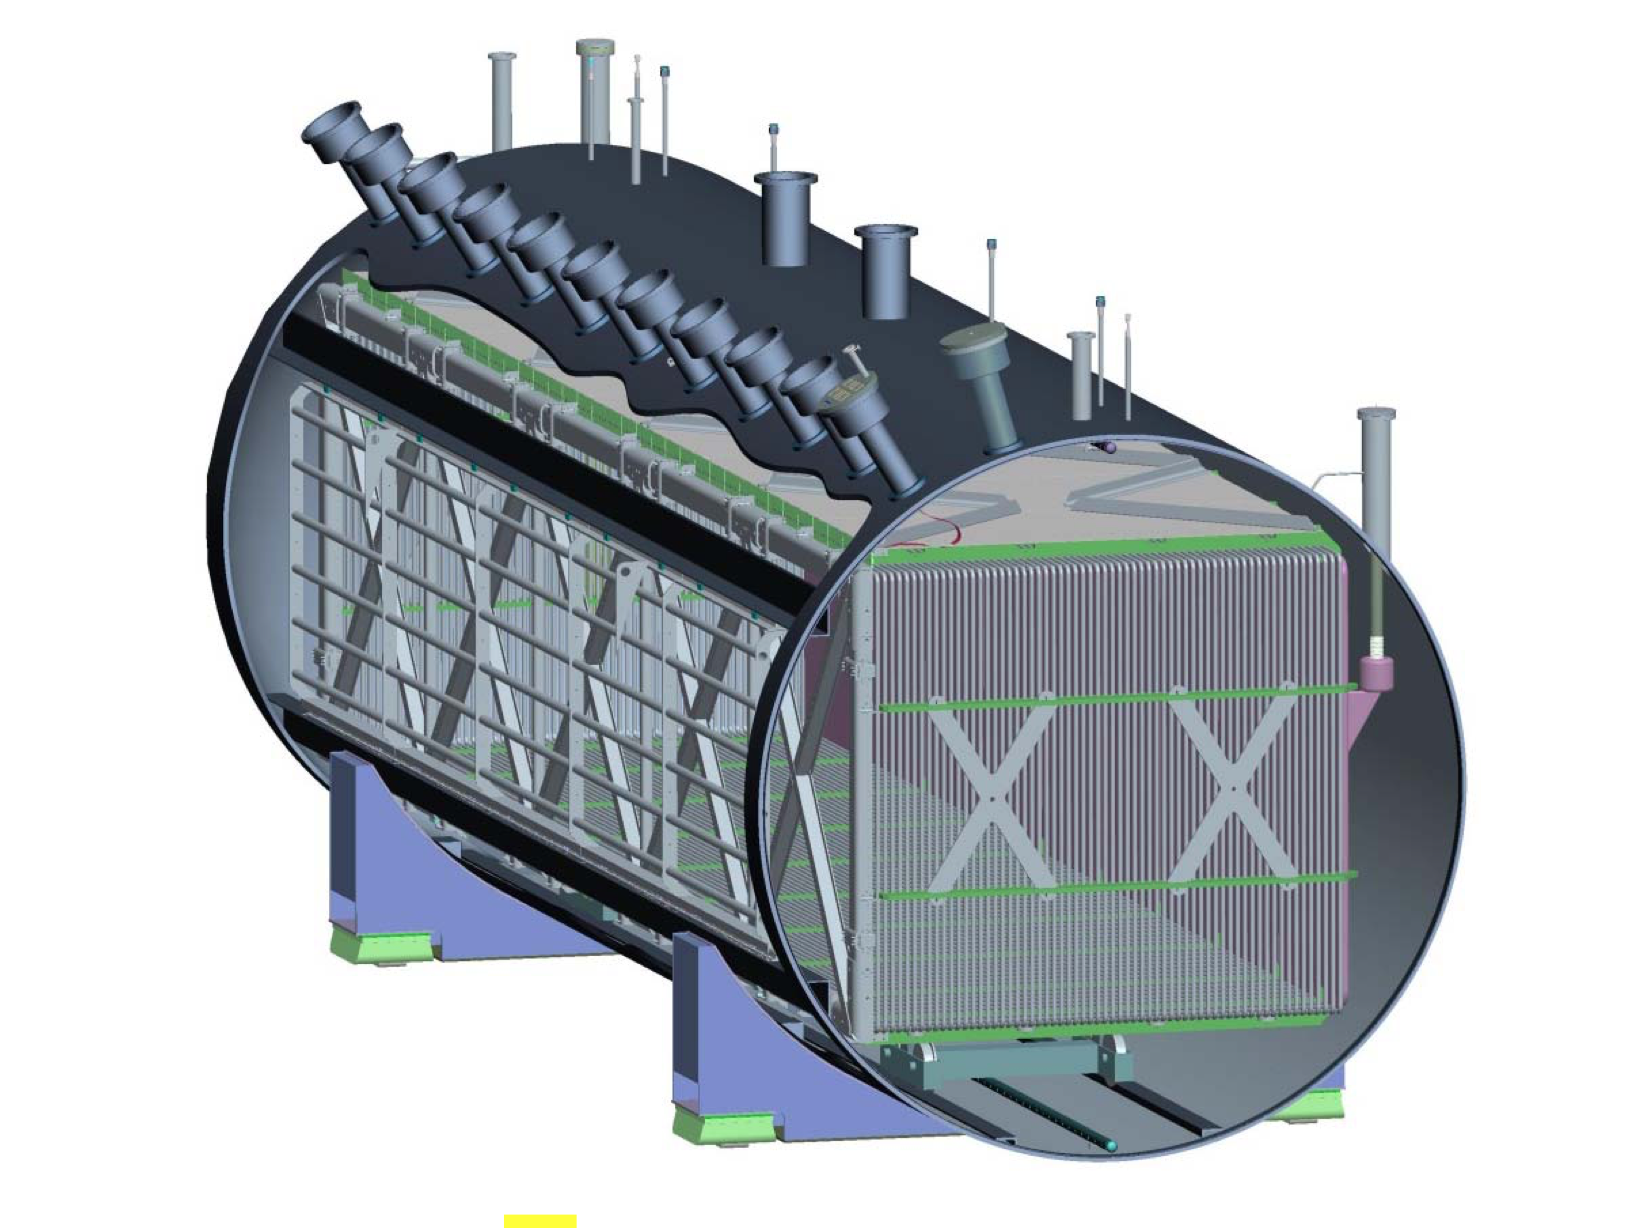
\includegraphics[scale=0.35]{Figures/uboone_cryo.png}
        \caption[MicroBooNE's LArTPC inside the cryostat]{{\textbf{MicroBooNE's LArTPC inside the cryostat}} \\ Schematic view of MicroBooNE's LArTPC inside of the cryostat vessel. The cryostat is the cylindric-like structure in the figure \cite{microboone_design}.}
        \label{uboone_cryo} 
    \end{center}
\end{figure}

\subsection{Light Collection System}

As mentioned in chapter \ref{Chapter:1}, the scintillation light produced by a charged particle crossing the LArTPC gives information about the event's start time. From the difference between the time that the electrons are collected in the collection plane and the start time of the event, plus the knowledge of the drift velocity of the electrons in the detector, we recover the third dimension of the track reconstruction. In MicroBooNE, the drift velocity of the electrons is $1.14$ m/ms. 

This is only possible because LAr produces plenty of scintillation light ($\approx 10^4 $) photons/MeV, and this light is produced and propagated in LAr almost instantaneously ($\approx$ ns). The scintillation light is produced in LAr by two mechanisms: self-trapped excitation luminescence and recombination luminescence. Figure \ref{lar_excimers} is a diagram demonstrating those two processes. When a charged particle passes through the liquid argon, it ionizes or excites it. In the first case, it will result in light being produced by self-trapped excitation luminescence, which will produce a singlet state in $65\  $ of the cases, and a triplet state in $35\%$ of the cases. In the excitation case, it will produce light by recombination luminescence, producing a singlet state in half of the cases and a triplet state in the other half. In all cases, the light signal is suppressed by impurities in the LAr. Either process produces light with a peak at the $128$ nm wavelength \cite{lar_excimers}.
 
\begin{figure}[h!]
    \begin{center}
        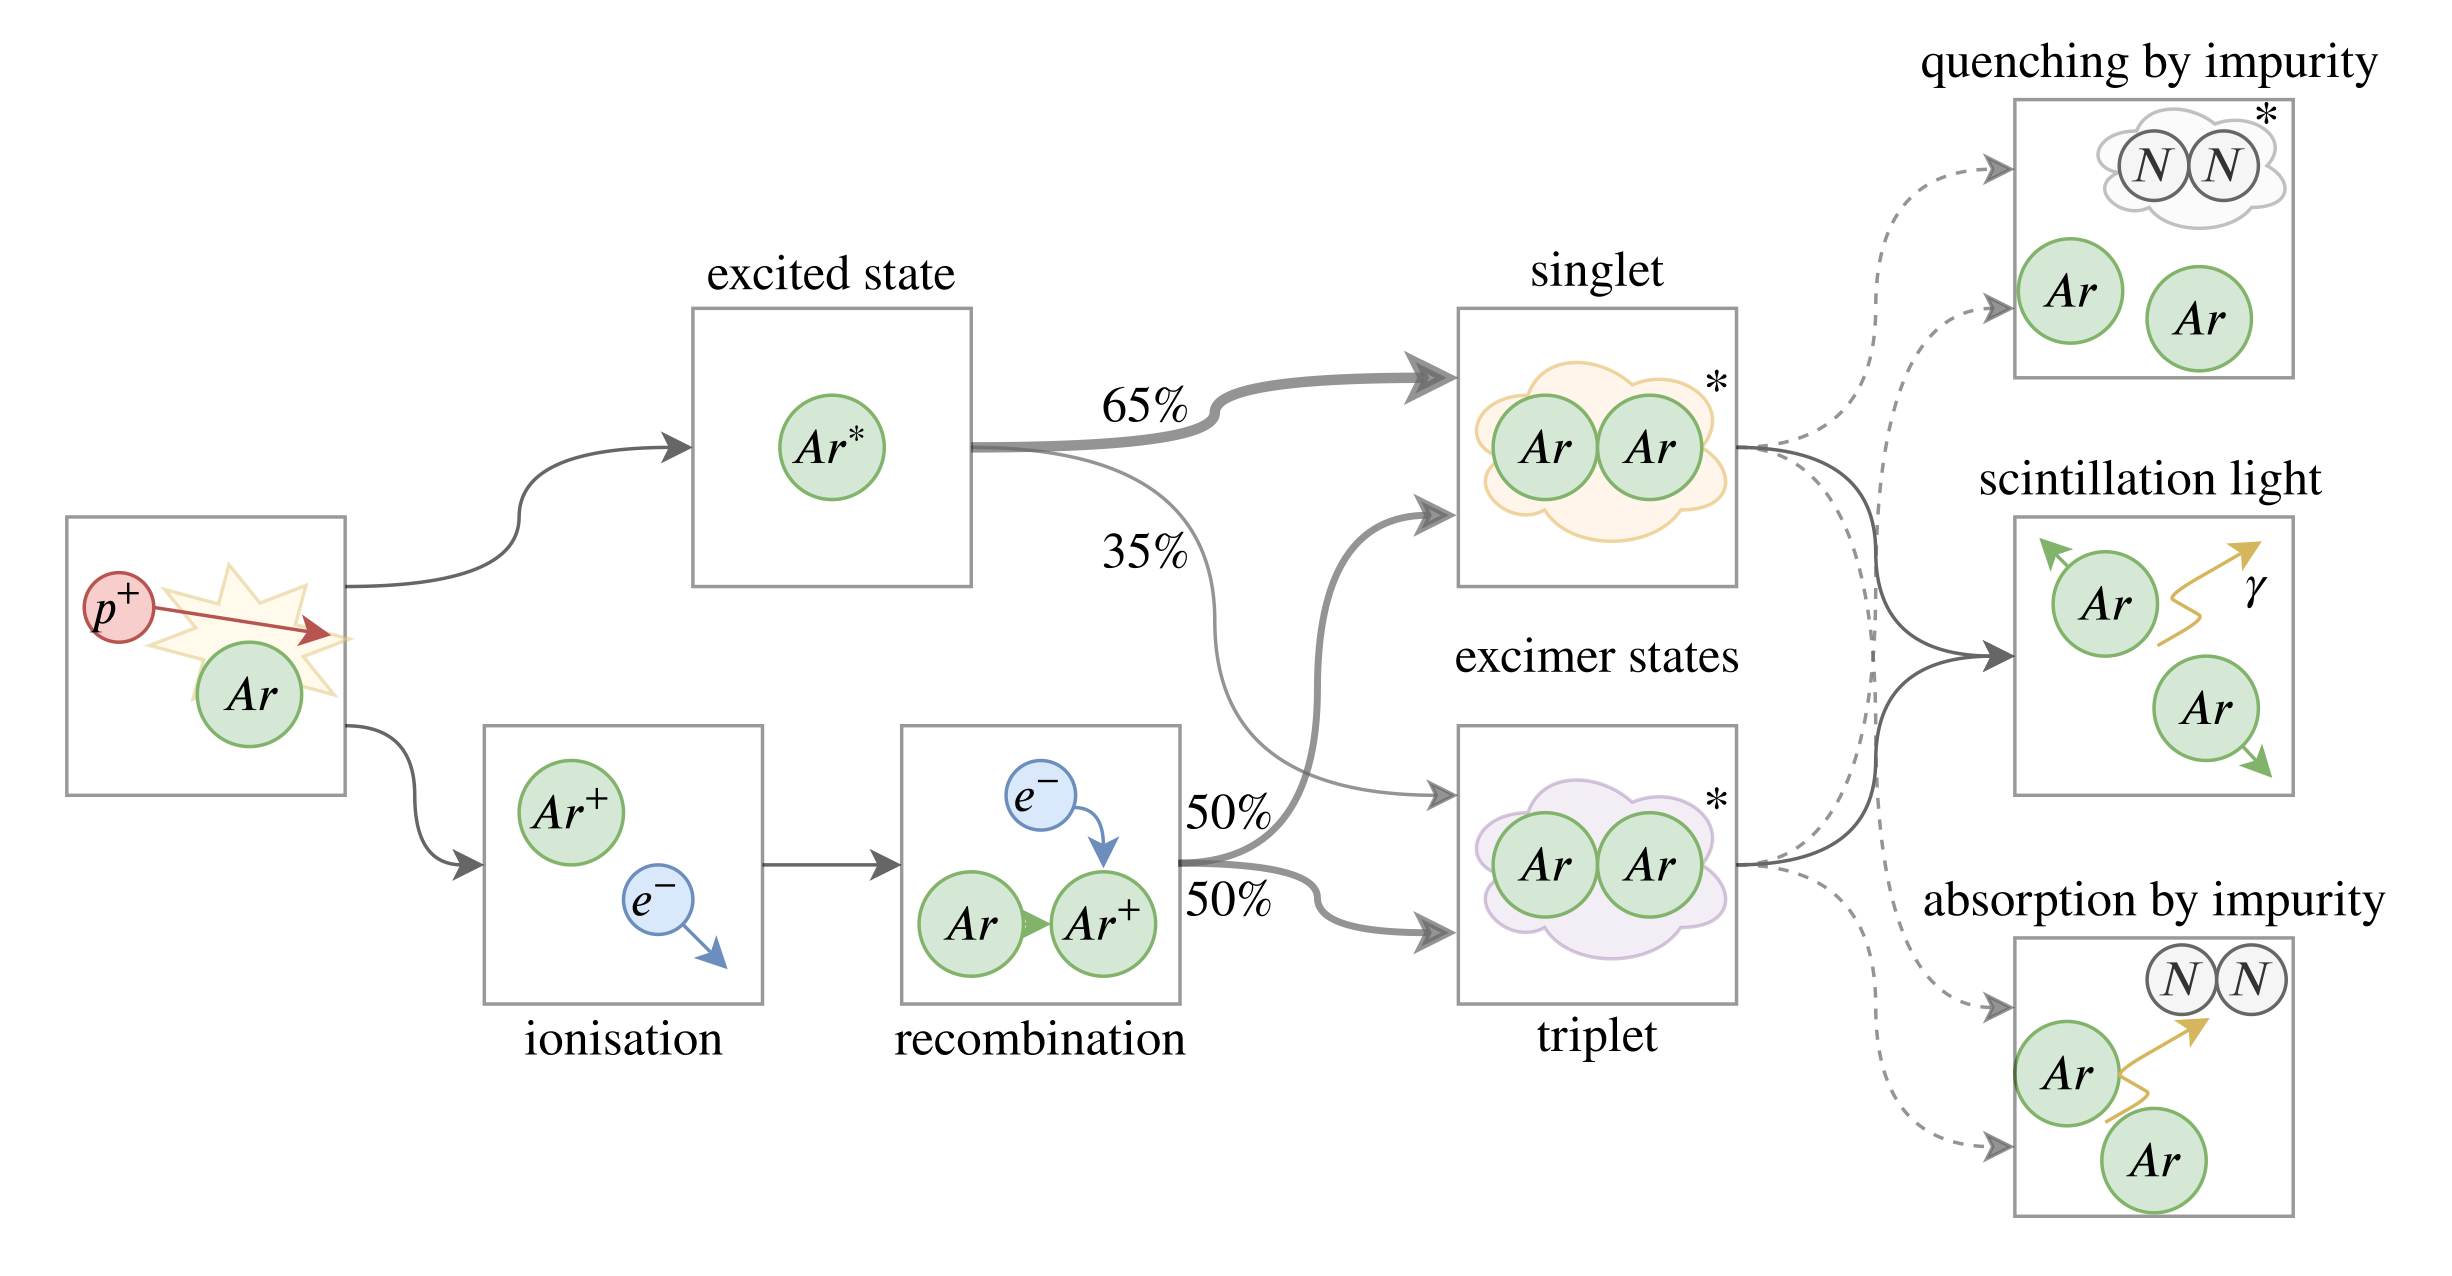
\includegraphics[scale=0.35]{Figures/lar_excimers.png}
        \caption[Scintillation light in liquid argon]{{\textbf{Scintillation light in liquid argon}} \\When a charge particle passes through the liquid argon, it ionizes or excites it. The light will be either produced by self-trapped excitationor by recombination. In all cases the light signal is supressed by impurities in the LAr \cite{lar_excimers}.}
        \label{lar_excimers} 
    \end{center}
\end{figure}
  
To detect this light signal, MicroBooNE has $32$ units of 8-inch Hamamatsu photomultiplier tubes (PMTs) arranged behind the APA. Each of them is covered with a plate coated in tetraphenyl butadiene (TPB) wavelength-shifter that absorbs the $128$ nm photons and re-emits them at $\approx425$ nm, which is compatible with the PMT's maximum quantum efficiency. A picture of a MicroBooNE PMT is in figure \ref{uboone_pmt}. Figure \ref{pmt_quantum_eff} shows the quantum efficiency of the PMTs used in MicroBooNE. 
  
\begin{figure}[h!]
    \begin{center}
        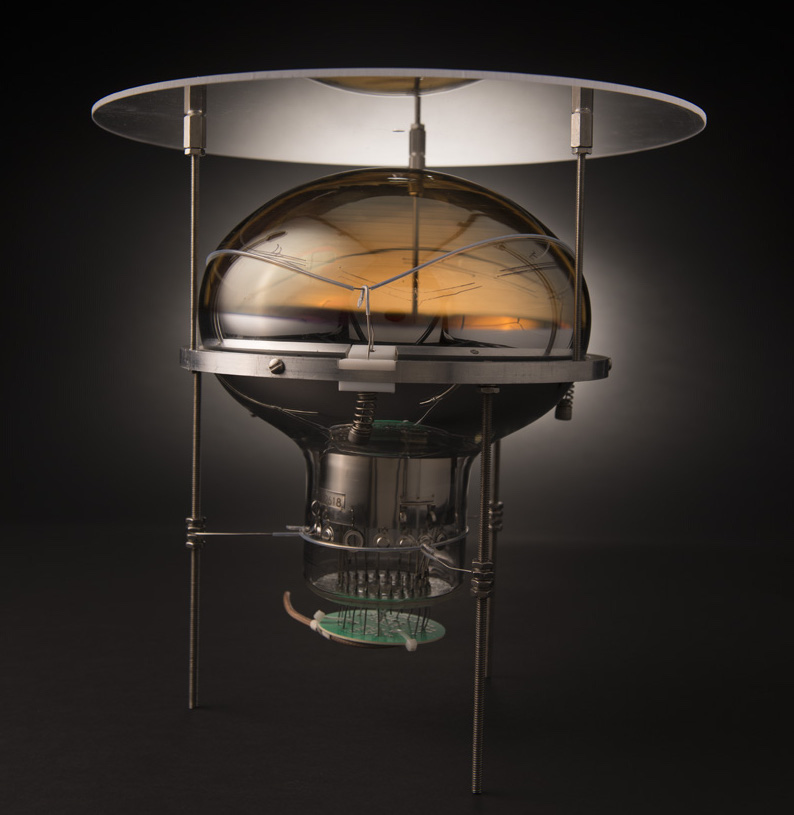
\includegraphics[scale=0.25]{Figures/microboone_pmt.jpeg}
        \caption[MicroBooNE's PMT]{{\textbf{MicroBooNE's PMT}} \\Picture of a $8$-inch Hamamatsu PMT used in MicroBooNE \cite{uboone_pmt}.}
        \label{uboone_pmt} 
    \end{center}
\end{figure}

\begin{figure}[h!]
    \begin{center}
        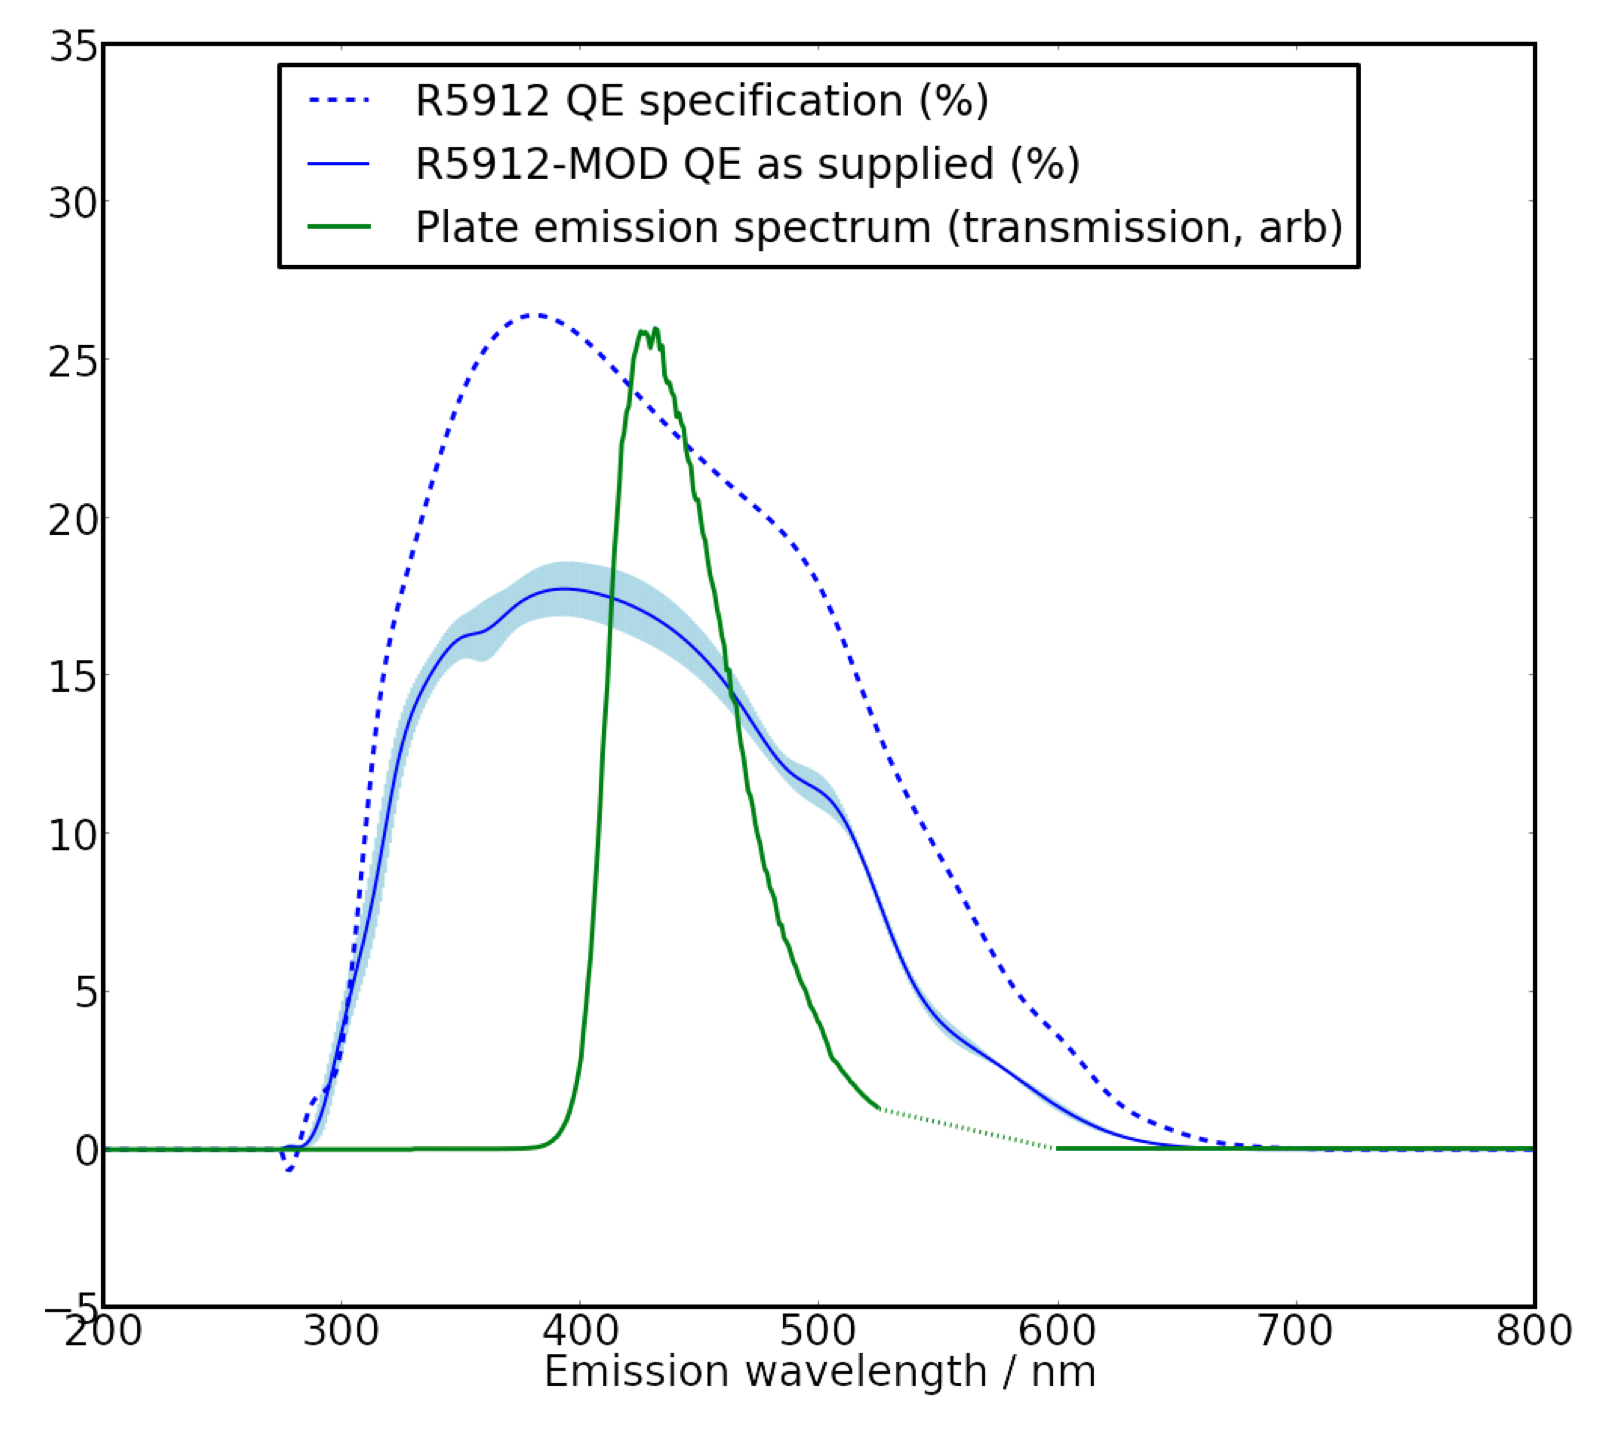
\includegraphics[scale=0.4]{Figures/quantum_eff.png}
        \caption[PMT's Quantum Efficiency]{{\textbf{PMT's Quantum Efficiency}} \\The specification for the non-platinum undercoated R5912 Hamamatsu PMT. The blue band shows the mean and standard deviation of the four quantum efficiency curves provided by Hamamatsu for the installed PMTs. Also shown is the measured emission spectra of the MicroBooNE wavelength-shifting coatings \cite{microboone_design}.}
        \label{pmt_quantum_eff} 
    \end{center}
\end{figure}
  

\section{Neutrino at the Main Injector (NuMI) Beamline}
  
To study neutrinos, Fermilab produces neutrinos through an accelerator chain that delivers two beams, the Booster Neutrino Beam and the Neutrino at the Main Injector beam. Both supply neutrinos to a variety of experiments. MicroBooNE's main beam is the BNB,  but it is also exposed to the NuMI beam. 
  
The accelerator chain (see full Fermilab's beam chain in figure \ref{accelerator_chain}) starts with an ion source machine with a molybdenum cathode installed inside of it and filled with hydrogen gas. The molybdenum's electrons are excited and then collected by the hydrogen atoms. The result is a H$^-$ gas. An ``extractor" attracts the negative atoms with a positive potential, pulling them through a hole with a width of a few mm. At the same time, a magnetic field guides them in the right direction to feed the beam into a radio-frequency quadrupole (RFQ). The RFQ receives the low-energy beam from the ion source at one end and ejects a $750$ keV \cite{RFQ_website} beam out of the other end, delivering it to a linear accelerator (LINAC). The LINAC is $150$ m long and is divided into two acceleration parts. The first is a drift tube that accelerates the beam up to $116$ MeV, and the second is a side-coupled cavity that accelerates the beam up to $401$ MeV \cite{LINAC_website}. Exiting the LINAC, the beam collides with a thin carbon sheet that removes electrons from the H$^-$, resulting in three beams: a $H^-$ beam, a $H^+$ beam, and a $H^0$ beam. Only the pure proton beam is selected. After these processes, the beam is suitable to be inserted into a circular $75$ m radius accelerator called the Booster, from which an $8$ GeV beam of protons is extracted that can be directed towards the Main Injector (MI), the BNB target, or to the Recycler \cite{booster_website}. For the NuMI beam, the protons from the Booster are directed towards a $3319.4$ m circumference synchrotron, called the Main Injector, that further accelerates the protons up to $120$ GeV. Those protons are then directed towards a graphite target, where they collide, producing the NuMI beam.
  
\begin{figure}[h!]
	\begin{center}
		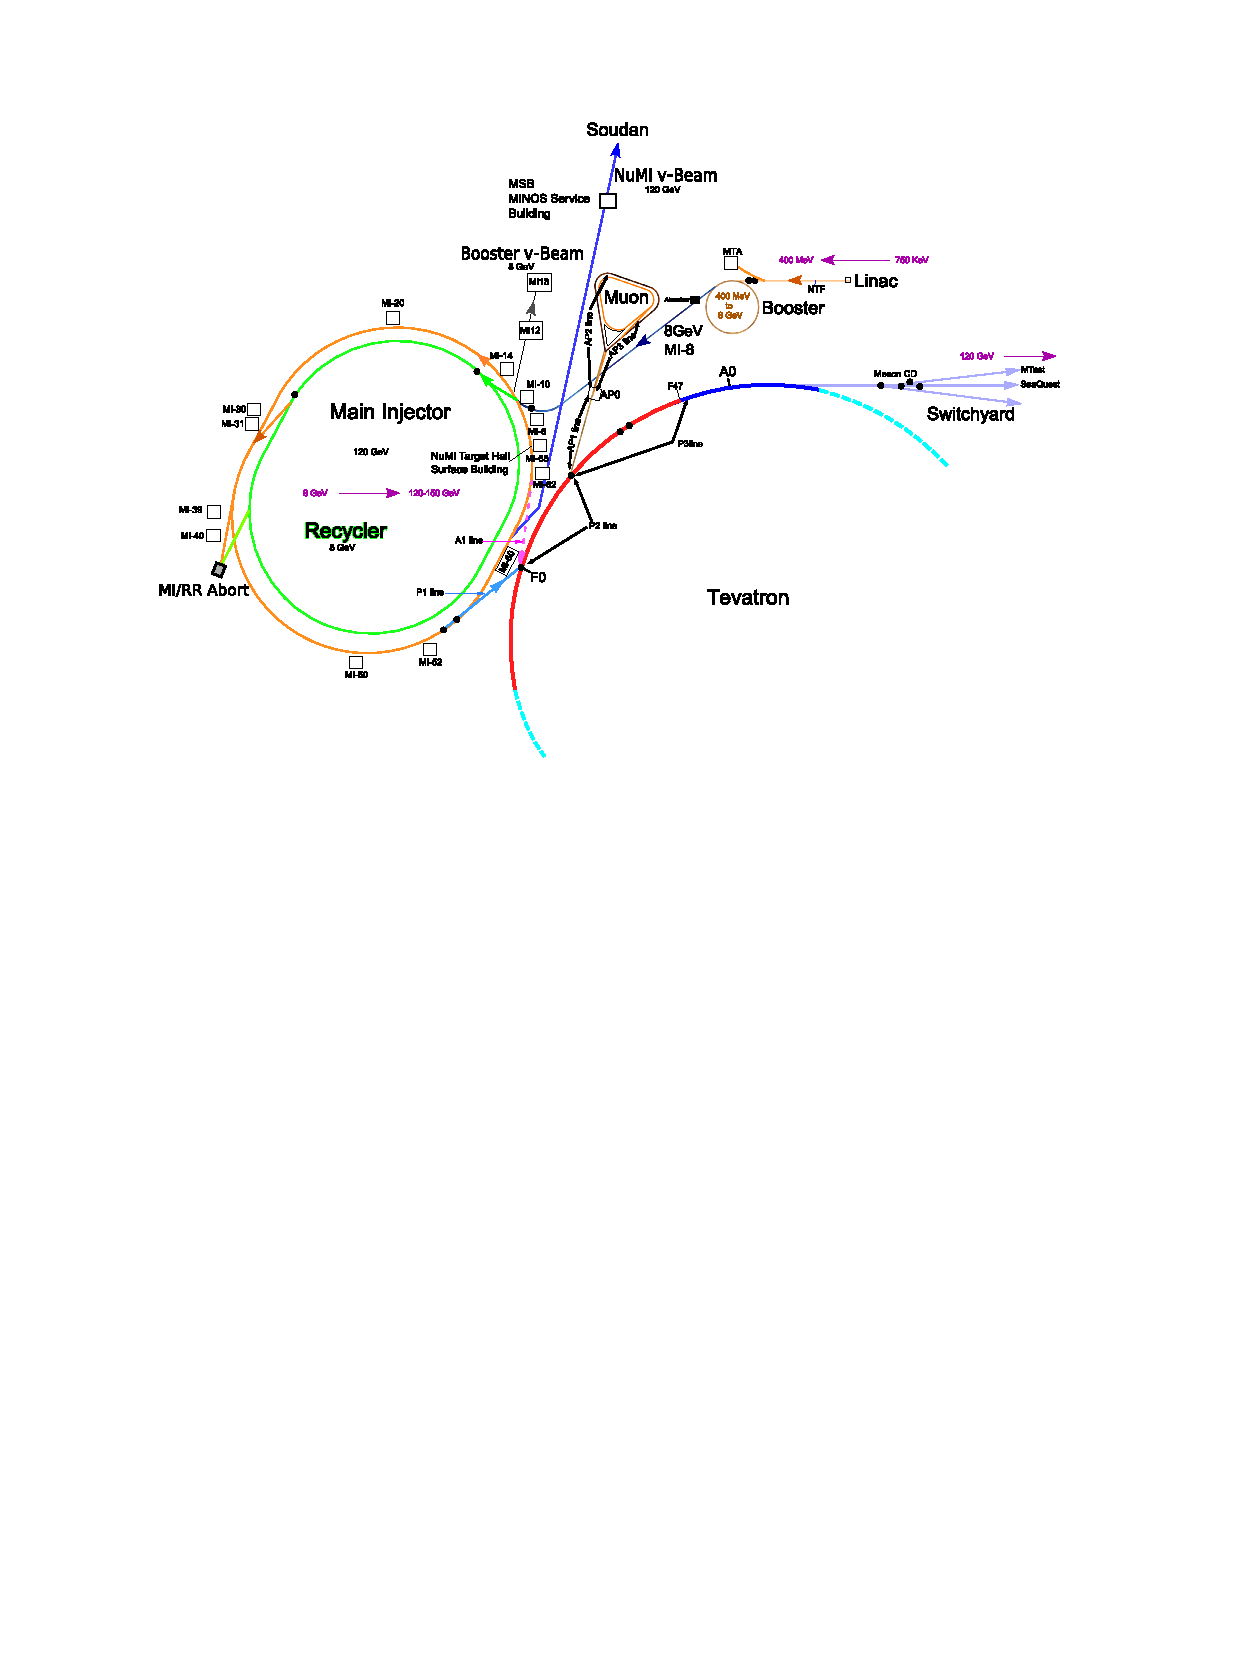
\includegraphics[scale=0.8]{Figures/acceleratorChain.pdf}
		\caption[Full Fermilab's beam chain]{ {\textbf{Full Fermilab's beam chain}} \\The image shows the Fermilab beam chain map, from the RFQ/LINAC to the main injector, BNB, or to the recycler \cite{paper_numibeamline}.}
		\label{accelerator_chain}	
	\end{center}
\end{figure}
  
In the NuMI beam, when the $120$ GeV protons impinge upon a graphite target, they produce mesons, including charged pions and kaons. These mesons are focused by magnetic horns and directed to the $675$ m long decay pipe, where they decay into muons and muon-neutrinos, as shown in the schematic view of the beamline in figure \ref{fig:numi}. After the decay pipe, an absorber blocks the remaining hadrons and muons in the beamline, allowing only the neutrinos to pass through. 
  
\begin{figure}[h!]
    \centering
    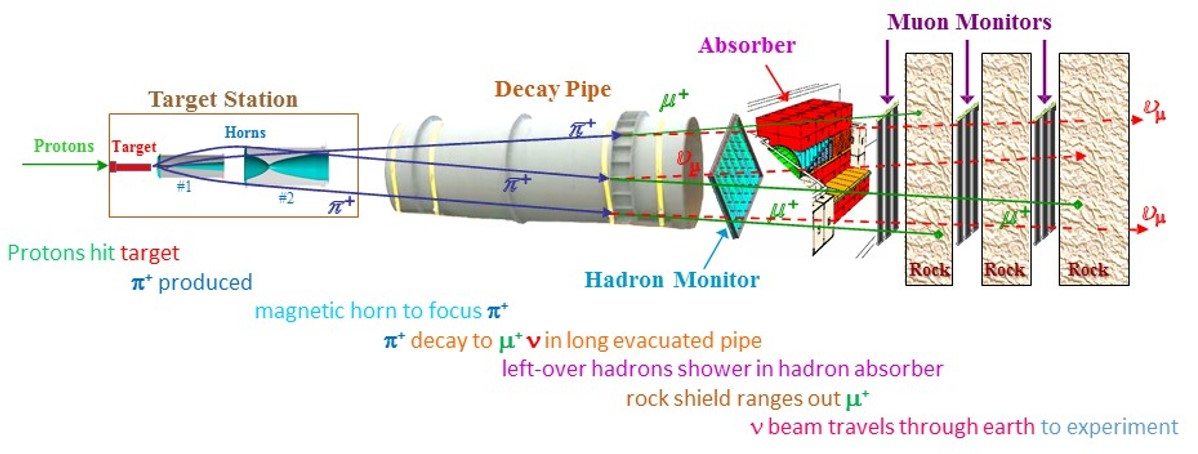
\includegraphics[width=140mm]{Figures/numi.jpg}
    \caption[NuMI layout]{{\textbf{NuMI layout}} \\Layout of the NuMI beamline \cite{numi}.}
    \label{fig:numi}
\end{figure}
  
By changing the polarity of the magnetic horns, we can select the sign of the charged mesons. By having a positive horn current, we select positive particles. We call it the Forward Horn Current (FHC) mode, or Neutrino Mode. By having a negative horn current, we select negative particles. We call it the Reverse Horn Current (RHC) mode, or Antineutrino Mode. In figure \ref{beam_mode_uboone} you can find a plot of the number of Protons on Target (POT) delivered in each run of MicroBooNE and in which mode the beam was selected. The NuMI beam delivers neutrinos in windows of $9.6 \mu$s. During MicroBooNE's operation time we collected a total of $2.3\times 10^{21}$ POT, $1.0\times10^{21}$ in Neutrino Mode and $1.3\times10^{21}$ in Antineutrino Mode
 
\begin{figure}[h!]
    \centering
    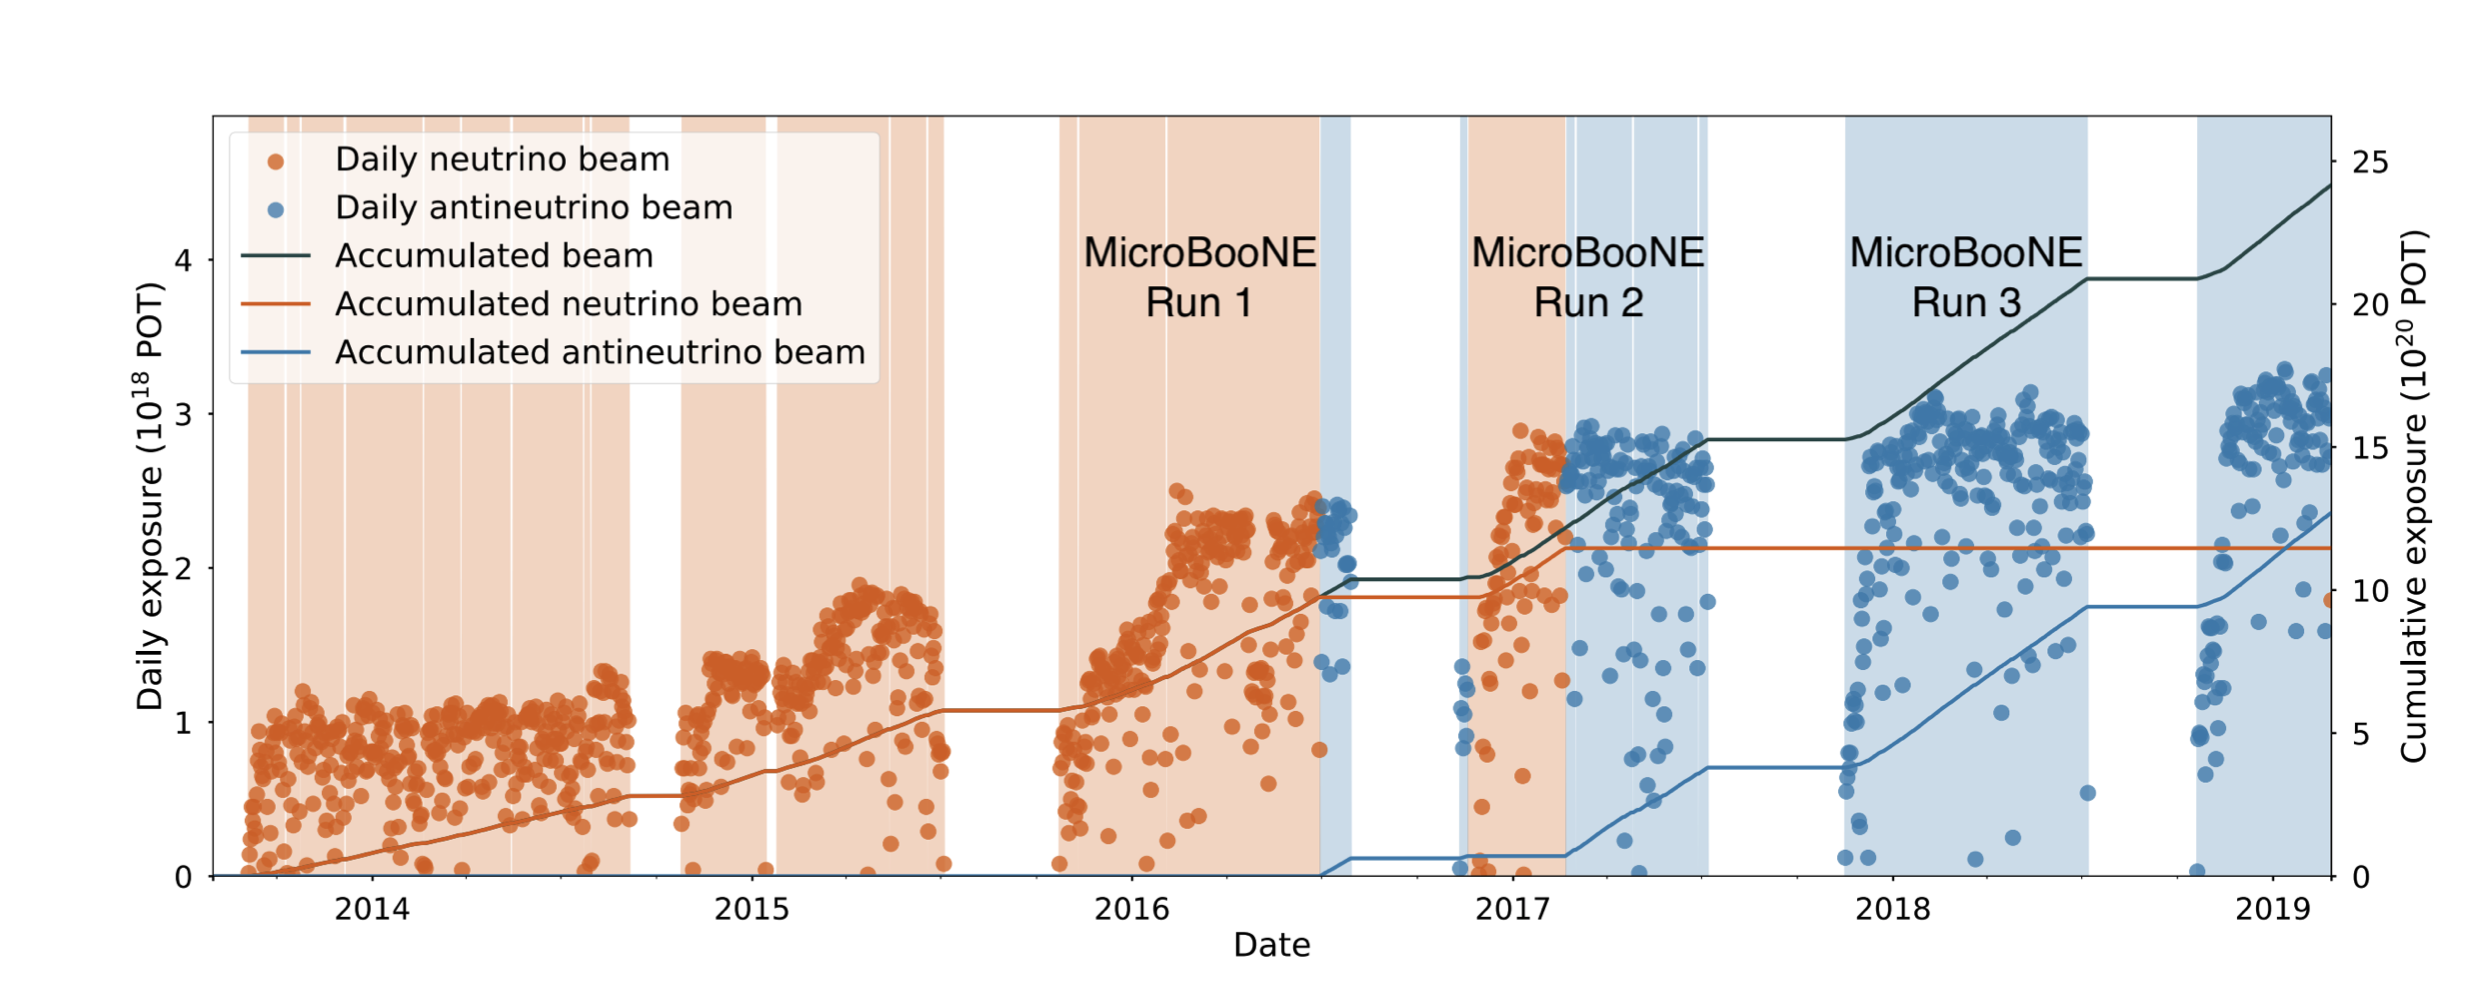
\includegraphics[width=150mm]{Figures/beam_mode_uboone.png}
    \caption[The total cumulative POT delivered by the NuMI beamline to MicroBooNE]{{\textbf{The total cumulative POT delivered by the NuMI beamline to MicroBooNE}}\\The cumulative POT from NuMI delievered to MicroBrooNE. In the orange regions the horn polarity was in Neutrino Mode. In the blue regions the horn polarity was in Antineutrino Mode. The white regions refer to periods in which the accelerator complex was shut down \cite{krish_phd}.}
    \label{beam_mode_uboone}
\end{figure}
  
\section{MicroBooNE's Readout and Trigger Systems}
  
As a surface detector, MicroBooNE's PMTs and TPC receive particle activity all the time, and recording all this data would be impossible. Additionally, only $2-3\%$ of the pulses of protons sent to the target (called ``spills") to produce the neutrinos in the NuMI beam will create a neutrino interaction in MicroBooNE. We use a trigger system to decide what data is recorded.
The trigger system starts with a signal from Fermilab's accelerator complex informing us they sent a new spill. This signal is our hardware (HW) trigger. The HW trigger gives a start to what we call the``beamgate window", in which we start the readout without any light intensity requirement (also known as ``unbiased"), which lasts $23.4$ $\mu $s. This happens $1.6$ ms into the TPC readout frame. The NuMI beam spill time window goes from $5.64- 15.44$ $\mu$s into the beamgate window. The complete readout cycle takes 3 TPC readout frames, which takes a total of $4.8$ ms.
The data collected is then passed to a buffer where a software will decide what will be permanently recorded on tape. This is our software (SW) trigger. To be recorded, the SW trigger requires the data to have at least $9.5$ PE of scintillation light in a time window of $4.69- 16.41$ $\mu$s from the beginning of the beamgate window. To account for some decline in the PMTs, during Run 3, the light requirement was updated to $5.75$ PE \cite{numi_redmine}. 
Around $14\%$ of all HW triggers pass the SW trigger conditions. 

Please see the diagram in figure \ref{trig} for a visual of the readout and trigger structure.

\begin{figure}[h!]
    \centering
    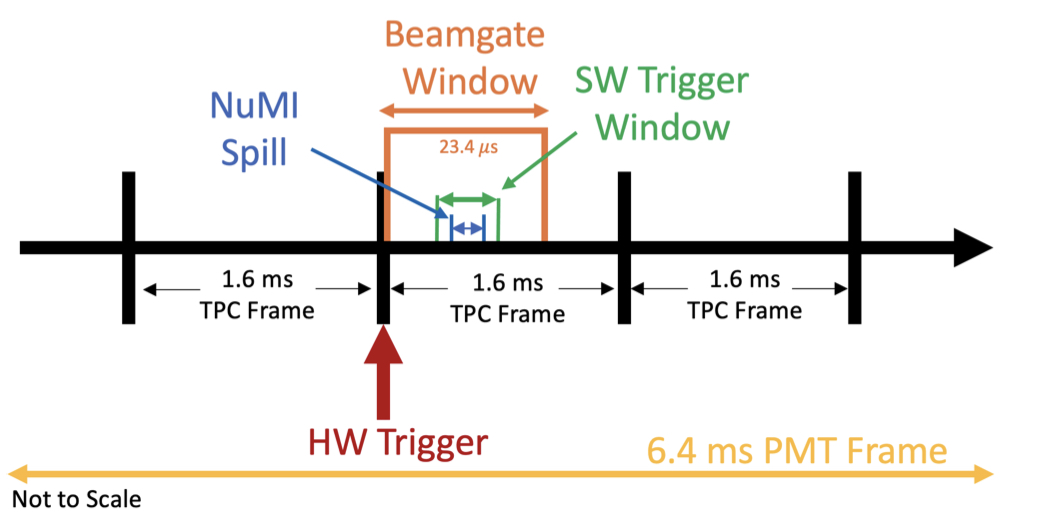
\includegraphics[width=150mm]{Figures/numi_trigger.jpg}
    \caption[MicroBooNE's NuMI readout and trigger]{\textbf{MicroBooNE's NuMI readout and trigger}\\Structure of MicroBooNE's NuMI readout and trigger \cite{krish_phd}.}
    \label{trig}
\end{figure}

From the data collected, MicroBooNE produces three data streams:
\begin{itemize}
 \item NuMI: For this stream, the data has to pass both the hardware and software triggers described above. It is also referred to as ``beam-on" data. 
 \item EXT NuMI: This is some data that passes the light requirements of the software trigger but is outside the beamgate window. The light is produced by cosmic rays, and this data is essential for us to understand the background of the neutrino analysis. It is also called ``beam-off" data. 
 \item EXT unbiased: This is data that is not in the beamgate window but with no additional requirements. Data from this stream is used to make our simulated events more realistic, as we overlay them with the simulated neutrino interactions. The procedure we use for that is documented in \cite{afro_phd}. 
\end{itemize}

MicroBooNE has a similar data stream, readout, and trigger systems for the BNB beam but with its own time windows. The beamgate window for the BNB and NuMI beams do not overlap. 

\chapter{$\mu$ Decay At Rest $\nu_{e}$-LAr CC Cross Section in MicroBooNE}
The only supernova neutrinos detected to date was the SN1987A, from a supernova that happened at the Large Magellanic Cloud. A small amount of electron neutrinos from the event were observed at Kamiokande-II ($12$ $\bar{\nu}_e$s), IMB ($8$ $\bar{\nu}_e$s), and Baksan ($5$ $\bar{\nu}_e$s). Despite the small dataset, a rich amount of analysis was published using the data, \cite{Kamiokande-II-PRL, Kamiokande-II-PRD, IMB, Baksan}. 
On the occasion of a core-collapse supernova in our galaxy, measuring the flux of neutrinos and antineutrinos from all flavors will significantly enlighten the fields of astrophysics and neutrino physics. Therefore, one of DUNE's goals is to be prepared for such an event, as it is the most potent detector to measure the electron neutrinos signal from a supernova, \cite{dune_SAND}.
In this chapter, I will explain the basics of supernovas and the neutrinos produced at them, why DUNE is particularly suitable to measure those neutrinos, and how using muos that decay at rest ($\mu$DARs) at the NuMI beam and interact in the MicroBooNE detector can help us improve neutrino-nucleus theoretical models and MeV-scale detection techniques in LArTPCs, which will be essential to accomplish the supernova detection in DUNE.

\section{Core-Collapse Supernova Neutrino Detection in DUNE}
\subsubsection{Supernovas}
Supernova is the name given to the explosive chain of events that happens during the death of some stars. Mainly, core-collapse supernovas produce a massive number of neutrinos and antineutrinos whose spectrum, if measured, can inform the characteristics of the explosion. 
At the end of the life of a star that has $8-40$ solar masses, its body is made of concentric shells that were formed at each of its previous burning phases, them being: hydrogen, helium, carbon, neon, oxygen, silicon, enveloping a core of nickel and iron. During its life, the stability of the star is a balance between the thermal pressure produced in the fusion process, which pulls everything in the outer direction, and its gravity pulling inward. When the mass of the iron core reaches $1.4$ solar masses, the pressure is not enough to balance the gravity, and the core starts to be compressed by its own weight. Temperature and density in the core rise and the reaction

\begin{equation}
    e^{-} + p \longrightarrow n + \nu_e
\end{equation}

starts to happen more frequently, causing the pressure from electrons to lower even more and the star to collapse more rapidly. At the latest stages of the collapse, the density is such that even neutrinos get trapped in the core. Eventually, the pressure created by the nucleons degeneracy interrupts the collapse. The sudden stop of the collapse in the core causes a shock wave through the outer layers, and the star explodes. At the early stage of the shock wave, the density lowers, and the neutrinos manage to escape, creating an intense few-millisecond pulse called neutronization burst. 
After the neutronization burst, outer layers of the star still falling innard manage to stall the shock wave briefly. This stage is called the accretion phase. We still don't understand why the shock wave regains energy enough to proceed. One hypothesis is that neutrino reactions produce sufficient heat for the thermal pressure to give continuity to the explosion. 
Next, in the cooling phase, the star's energy is given away in many different processes that create neutrinos and antineutrinos of various flavors. A few of them are:

\begin{align}
    & \text{{\color{gray} electron pair annihilation:}}
    && e^{-} + e^{+} \longrightarrow \nu + \bar{\nu}, \\
    & \text{{\color{gray}electron-electron neutrino bremsstrahlung:}}
    && e^{\pm} + e^{\pm} \longrightarrow e^{\pm} + e^{\pm} + \nu + \bar{\nu} \\
    & \text{{\color{gray}electron-nucleon neutrino bremsstrahlung:}}
    && e^{\pm} + N \longrightarrow e^{\pm} + N + \nu + \bar{\nu} \\
    & \text{{\color{gray}photoannihilation:}}
    && \gamma + e^{\pm} \longrightarrow e^{\pm} + N + \nu + \bar{\nu} \\
    & \text{{\color{gray}nuclear de-excitation by neutrino pair production:}} 
    && ^{Z}_{A}X^{*} \longrightarrow ^{Z}_{A}X + \nu + \bar{\nu}
\end{align}

Given the wide variety of processes, measuring the flux of neutrinos and antineutrinos from all flavors is fundamental to help us better understand aspects of the supernova and what role the processes during the explosion play in its development, \cite{Gardiner_thesis}. 

\subsubsection{Supernova detection in DUNE}

We have in operation or planned for the future a number of large detectors that would be able to detect signals from a core-collapse supernova that happens in our galaxy. The active material of those detectors is either water Cherenkov or hydrocarbon scintillator, making them mainly sensitive to electron antineutrinos via inverse beta decay (the reaction in equation \ref{inverse_beta_decay_eq}). 
Therefore, relying solely on those detectors would limit the measurement of the supernova electron neutrino flux, which is the most significant component produced during the supernova's neutronization phase. 

Luckily, DUNE's active material is liquid argon, which is mainly sensitive to eletron neutrinos, via charged current scattering in $^{40}$Ar, as in:

\begin{equation}
    \nu_e + ^{40}Ar \longrightarrow ^{40}K + e^{-}
    \label{nu_scatter_eq}
\end{equation}
 
An example of a contribution to neutrino physics that a supernova neutrino detection could make in DUNE is to shine light into the mass ordering puzzle. Figure \ref{dune_supernova} shows how the time distribution of the incoming flux of the neutrinos of a $10$ kpc supernova in DUNE could depend on the mass hierarchy. In the case of inverted hierarchy, we should see an early excess of events from the neutronization phase, whether, in the case of normal hierarchy, we should see the absence of such events. The results from figure \ref{dune_supernova} are made assuming a model describer in reference \cite{dune_supernova_model}, but those results are assumed to be fairly model-independent \cite{kate_scholberg}. 

\begin{figure}[h!]
    \centering
    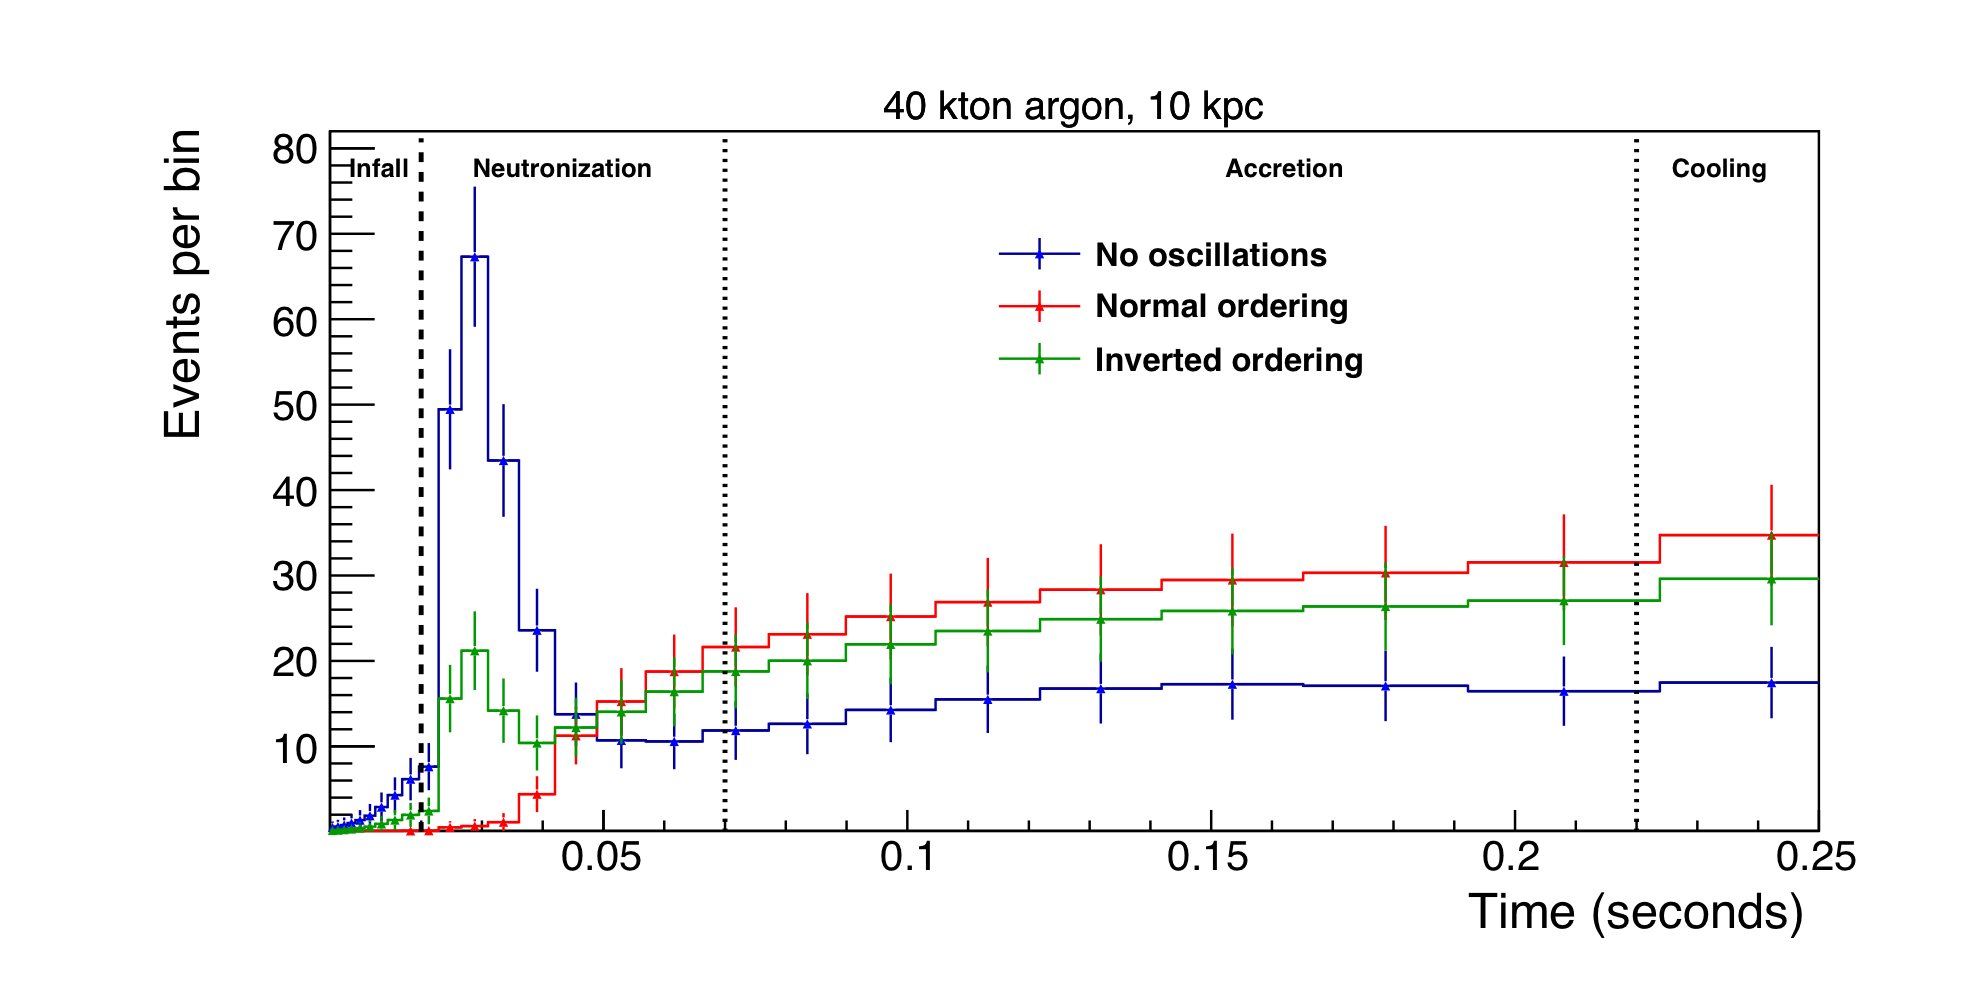
\includegraphics[width=150mm]{Figures/dune_supernova.jpeg}
    \caption[Predicted event time distribution for the detection of supernova neutrinos in a DUNE-like $40$ kt LArTPC]{{\textbf{Predicted event time distribution for the detection of supernova neutrinos in a DUNE-like 40 kt LArTPC}}\\ Predicted event time distribution for the detection of a $10$ kpc supernova neutrinos in a DUNE-like 40 kt LArTPC for each of the supernova stages. The blue curve assumes no oscillations, the green and the red curves assume oscillations for inverted and normal mass hierarchy, respectively \cite{kate_scholberg}.}Furthermore, being able to measure the flux of both neutrinos and antineutrinos is fundamental to further understanding exotic supernova processes \cite{Friedland}.
    \label{dune_supernova}
\end{figure}

Furthermore, being able to measure the flux of both neutrinos and antineutrinos is fundamental to further understanding exotic supernova processes \cite{Friedland}. 

\section{$\mu$ Decay At Rest $\nu_e$ Charged Current interactions in MicroBooNE}

\subsection{$\mu$ Decay At Rest in MicroBooNE}
As promising as the DUNE supernova neutrino program is, we currently lack an understanding of the MeV-scale neutrinos and LAr nucleus interactions, LArTPC reconstruction capabilities, and event identification at this energy range. 

As mentioned before, MicroBooNE is exposed to the BNB and NuMI beamlines. Both beamlines produce a copious amount of antimuons that will, when decaying at rest, produce a muon antineutrino, an electron neutrino, and a positron, as shown in equation \ref{mudar_decay_eq}. The energy spectrum of the electron neutrinos from this decay is well-known and can be seen in picture \ref{mudar_nue_energy}. In figures \ref{numi_nue_flux} and \ref{numi_nu_flux} you can see the NuMI flux prediction of $\nu_e$s in MicroBoone by parents and the NuMI flux prediction in MicroBooNE of all neutrinos, respectively. 

\begin{equation}
	\mu^{+} \longrightarrow e^{+} + \nu_e + \bar{\nu}_{\mu}
    \label{mudar_decay_eq}
\end{equation}

\begin{figure}[h!]
    \centering
    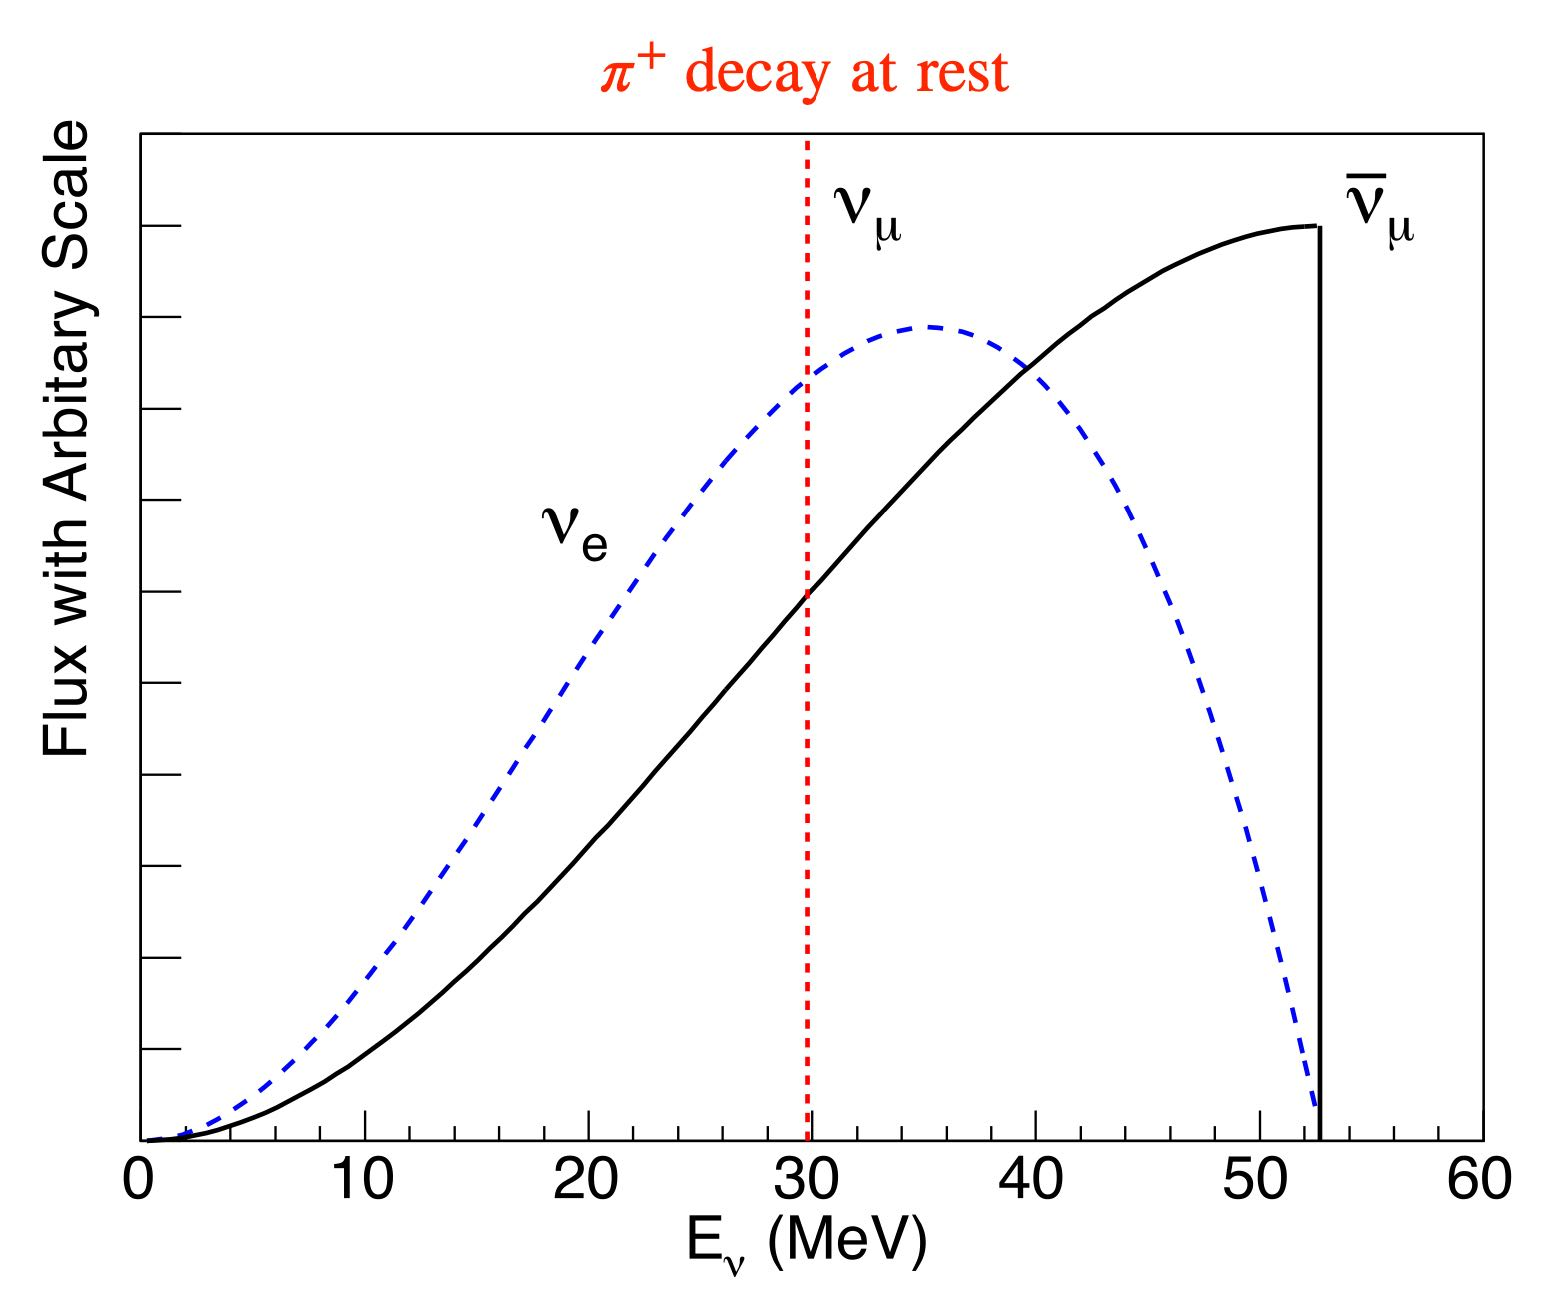
\includegraphics[width=110mm]{Figures/mudar_nue_energy.jpg}
    \caption[Neutrino spectra of pion and muon decay at rest]{{\textbf{Neutrino spectra of pion and muon decay at rest}}\\ The red line is the energy of muon neutrinos from pion decay at rest, which is well-defined. The blue and the black lines refer to the energy spectrum of electron neutrinos and muon antineutrinos from positive muon decay at rest, respectively \cite{Yang2012}.}
    \label{mudar_nue_energy}
\end{figure}

Due to the nature of the decay, the electron neutrino will have kinetic energy $0 \leqslant KE_{\nu_e} \leqslant 52.8$ MeV, which overlaps nicely with the energy range of the supernova electron neutrinos we aim to detect in DUNE!

\begin{figure}[h!]
    \centering
    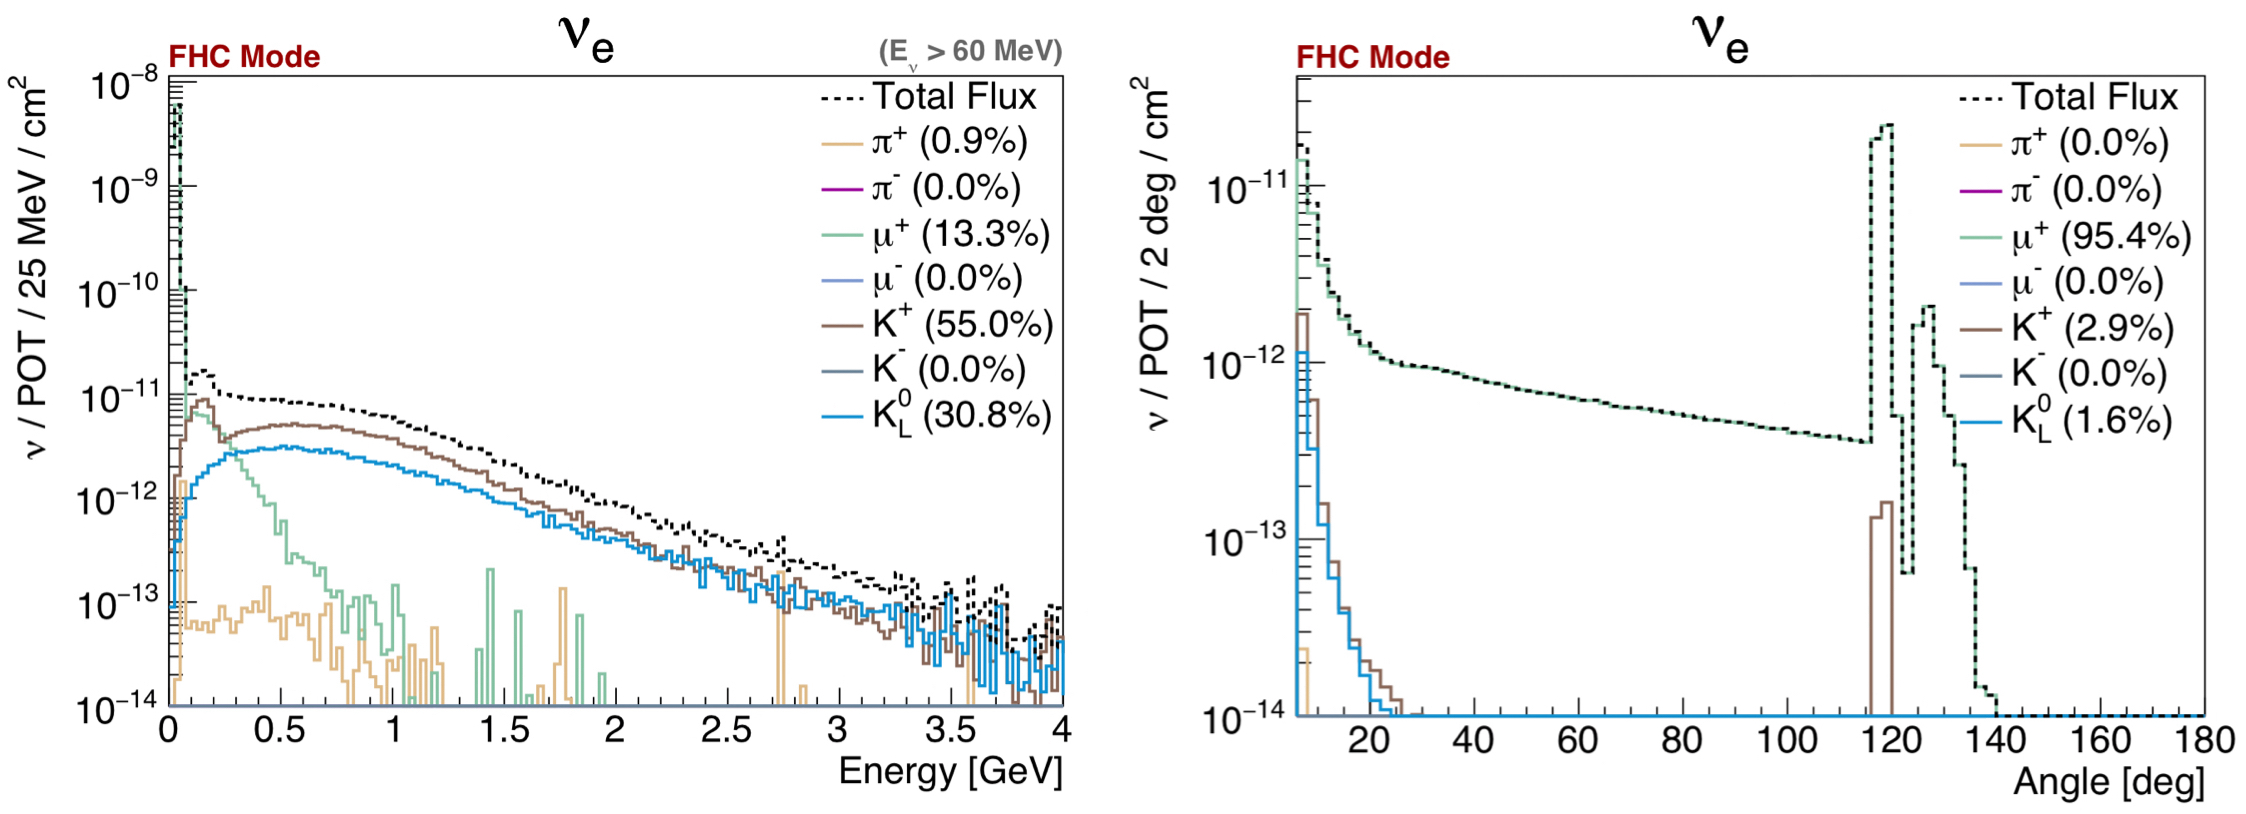
\includegraphics[width=180mm]{Figures/numi_nue_flux.jpeg}
    \caption[NumI $\nu_e$ flux in MicroBooNE]{{\textbf{NumI $\nu_e$ flux in MicroBooNE}}\\ On the right, the FHC $\nu_e$ neutrino flux at MicroBooNE from NuMI broken down by parent. Although a 60 MeV threshold is included in the percentages, the absolute value clearly shows the dominance of muon decays. On the left, the FHC neutrino flux is broken down by parent for each neutrino flavor. The percentages shown do not include an integration threshold on the angle. Decays from pions and muons dominate the majority of the flux across all angles \cite{krish_phd}.}
    \label{numi_nue_flux}
\end{figure}

\begin{figure}[h!]
    \centering
    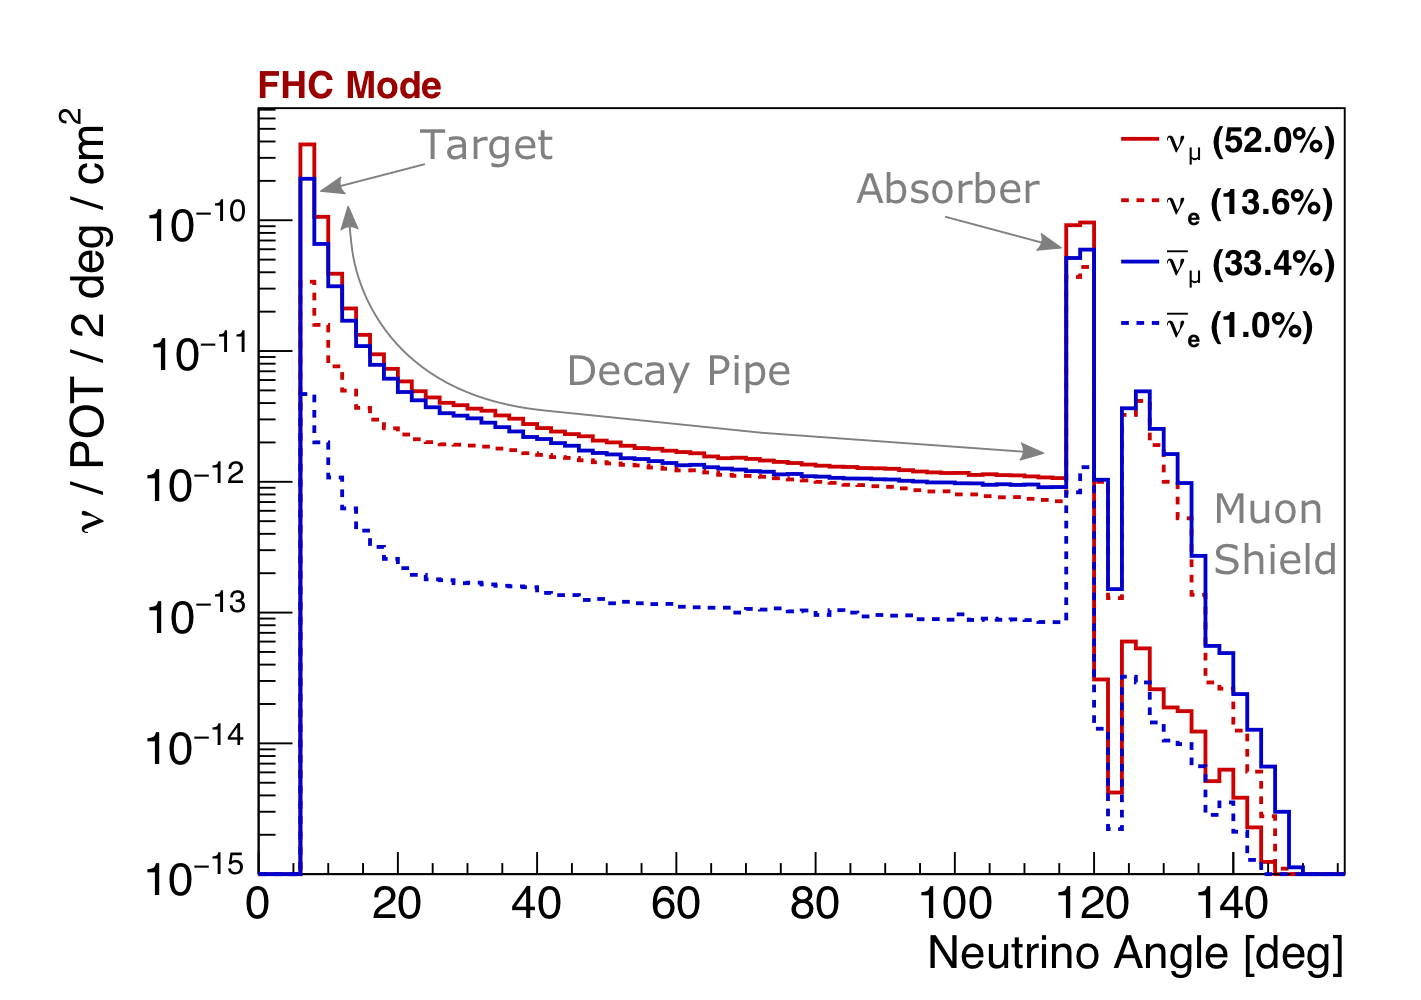
\includegraphics[width=130mm]{Figures/numi_nu_flux.jpeg}
    \caption[NumI $\nu$ flux in MicroBooNE]{{\textbf{NumI $\nu$ flux in MicroBooNE}}\\ The flux prediction for all neutrino flavours in the FHC mode in neutrino angle. No integration threshold is applied in the percentages, and the electron neutrino flux percentage is boosted by muon decay at rest. The large angular spread in the flux is due to the positioning of MicroBooNE with respect to the NuMI beamline. The flux peaks at the target location and tails off further into the beamline. From angles above $20$ deg (midway into the decay pipe), the flux remains flat up to the absorber, where there is a large peak in the flux spectrum $\approx 120$ deg. After this, the flux is attenuated rapidly going into the muon-shield $ \ge 120$ deg.\cite{krish_phd}.}
    \label{numi_nu_flux}
\end{figure}

\subsection{MeV-scale $\nu_e$-LAr Charged Current Interactions}

As explicitly shown in the \ref{nu_scatter_eq}, when MeV-scale neutrinos scatter in $^{40}$Ar, we have as product a $^{40}\textrm{K}^{*}$ and a $e^{-}$. From now on, I will refer to this electron as the ``main" electron of the signal. The energy of the incoming neutrino can be reconstructed as:

\begin{equation}
    E_{\nu} = E_e + \Delta_{final-initial} + T_{recoil} 
    \label{E_mudar_nu}
\end{equation}

where $E_e$ is the total energy of the outcoming electron and $T_{recoil}$ is the kinetic energy of the recoiling nucleus (which is negligible). As for $\Delta_{final-initial}$: 

 \begin{equation}
    \Delta_{final-initial} \equiv m_{final} - m_{initial}  
    \label{delta_fi}
\end{equation}

where $m_initial$ is the mass of the initial $^{40}$Ar nucleus, and $m_{final}$ is the mass state of the $^{40}\textrm{K}^{*}$ nucleus. The potassium nucleus can be at different excited states, depending on the event. Therefore, $m_{final}$ can be further described as:

\begin{equation}
    m_{final} = m_{final, g.s.} + E_x
    \label{mfinal}
\end{equation}

where $m_{final, g.s.}$ is the ground-state mass of a $^40$K nucleus and $E_x$ is the excitation energy. To reconstruct the total energy from the incoming neutrino, we need to look into the products from the de-excitation of the excited potassium nucleus, which are most commonly photons. Those photons can be indirectly measured in LArTPCs as they scatter on Ar atomic electrons, and the value of $\Delta_{final-initial}$ is given by:

\begin{equation}
    \Delta_{final-initial} = m_{g.s. \rightarrow g.s.} + \sum_{j}E_{\gamma, j}   
    \label{delta_fi_2}
\end{equation}

where $E_{\gamma,j}$ is the energy of each of the photons emitted and $m_{g.s. \rightarrow g.s.}$ is the mass difference between the ground state of the $^{40}$K nucleus and the ground state of the $^{40}$Ar nucleus, which is $1.5044$ MeV. 
It is also possible, although less likely, to have the excitation energy of the $^{40}$K high enough such that the de-excitation proceeds with the emission of a nucleon. A few of these channels still leave the daughter nucleus in an excited state, and there is an additional $\gamma$-ray or nucleon emission. This cascade continues until the daughter nucleus reaches the ground state. A diagram representing the different de-excitation channels can be seen in figure \ref{40K_deexcite}

\begin{figure}[h!]
    \centering
    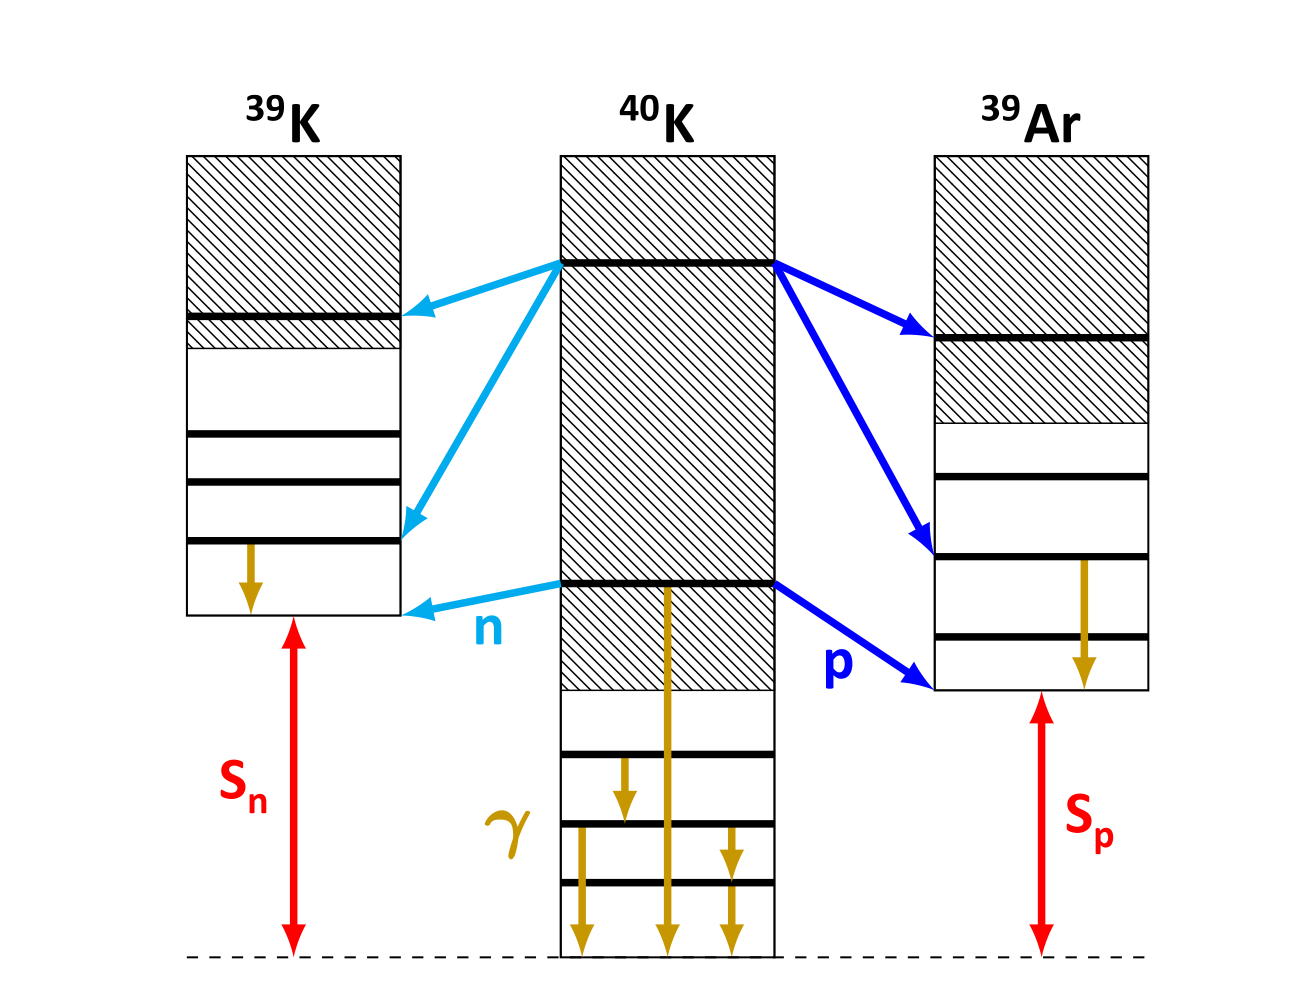
\includegraphics[width=135mm]{Figures/40K_deexcitation.jpeg}
    \caption[De-excitation channels from an excited $^{40}$K nucleus, product of a CC MeV-scale $\nu_e$-LAr scattering]{{\textbf{De-excitation channels from an excited $^{40}$K nucleus, product of a CC MeV-scale $\nu_e$-LAr scattering}}\\  The excited $^{40}$K nucleus can reach its ground state by emitting $\gamma$-ray(s) (middle diagram), a neutron (diagram on the left), or a proton (diagram on the right). In case the emission of a nucleon still leaves the daughter nucleus in an excited state, more photons are emitted until the ground state is reached \cite{Gardiner_thesis}.}
    \label{40K_deexcite}
\end{figure}

The complexity of nuclear structures and the possible final state topologies for those interactions add challenges to the proper energy reconstruction of the supernova neutrino events. Therefore, it is fundamental that we take the opportunity presented by $\mu$DAR $\nu_e$s in MicroBooNE to study these interactions to improve our techniques. 


\section{Simulation of $\mu$DAR Events in MicroBooNE}

To properly evaluate the $\mu$DAR events in MicroBooNE, we count with a chain of different simulation software to mimic the particle production and interactions at each step of the way, from the early stages of the beamline to MicroBooNE's detector response. 
To explicitly name the sequence, we start at the NuMI beam flux simulation, to the Generates Events for Neutrino Interaction Experiments (GENIE) Generator, and to the Model of Argon Reaction Low Energy Yields (MARLEY) Generator, back to the GENIE again, then to Geant4. All these softwares are integrated into a larger framework called the Liquid Argon Software (LArSoft). I will further go over each of these in this section. 

\subsection{Geant4}

 Geant4 \cite{g4} is a software toolkit that simulates the interaction of particles with matter. It can handle electromagnetic, decay, and hadronic physics interacting with complex geometries and variable EM fields. In MicroBooNE we use it during two steps of the simulation chain I described above: the NuMI beamline, and the propagation of the neutrino-LAr interaction products through LAr.

\subsection{NuMI Beam Simulation}

The NuMI beam flux simulation software has been continually developed by several experiments that use the NuMI beam, such as No$\nu$A, Main Injector Neutrino ExpeRiment to study $\nu-$A interactions (MINER$\nu$A) \cite{minerva}, and Main Injector Neutrino Oscillation Search (MINOS \cite{minos}. The software simulates the proton-target collision and its products, hadrons and muons that decay into neutrinos. MicroBooNE has two Geant4 packages that can used in the NuMI beamline simulation to handle different physics models to describe the hadron production: the g4numi\_flugg and the g4numi. In the g4numi\_flugg, FLUKA software framework is used to model the hadron production and Geant4 is used to handle the geometry of the beamline \cite{fluka}. In the g4numi, Geant4 is used for both model the hadron production and to handle the beamline geometry. In this thesis, we used the latter. 
The NuMI beam simulation also uses the Package to Predict the FluX (PPFX) to constrain the hadron production modeling and also propagate uncertainties through the beamline simulation \cite{ppfx}. Detailed description on the full NuMI beamline flux simulation can be found at \cite{krish}. 

Historically, both the NuMI beam and the BNB beam flux simulation had a minimum lower incoming neutrinos energy of $60$ MeV. This lower threshold was removed in the NuMI simulation, which, together with the higher flux of MeV-scale neutrinos, is why we opted to first perform this analysis using the NuMI beam instead of the BNB beam. 

\subsection{GENIE and MARLEY}
GENIE and MARLEY are software that falls in a specific category called ``neutrino event generators” and is specialized in neutrino-nucleus interactions. They are equipped with theoretical models of neutrino-nucleus interactions across a wide range of energies and targets. 
GENIE is the standard event generator used by MicroBooNE for physics analysis. In it, the target nucleus is modeled as a relativistic Fermi gas, i.e., non-interacting nucleons confined in a constant potential well. This makes it unfit to mimic the neutrino-nucleus interactions at the MeV-scale since the nuclear level structure is relevant for the characteristics of our final products, as described in the previous section. 
MARLEY, on the other hand, was designed to be especially capable of handling low-energy neutrino-nucleus interactions. It is based on a formalism to calculate low-energy neutrino-nucleus scattering called Walecka-Donnelly \cite{Walecka-Donnelly}. In it:
\begin{enumerate}
 \item the field gauge boson is neglected, and the effective interaction Hamiltonian density at low energies is written as the leptonic current times the nuclear current.
 \item the impulse approximation is taken, i.e., it is assumed that the matrix elements of the total nuclear current are the sum of the current of all the individual nucleon terms.
 \item it is written down the most general form of the single-nucleon current operator consistent with symmetry constraints. An approximation to a given order (usually up to the first) is taken.
 \item a multipole expansion of the nuclear current is performed \cite{Gardiner_thesis}. 
\end{enumerate}

In the end, the cross-section is given by matrix elements of seven independent multipole operators, three for the vector current and four for the axial-vector current. 
Then, the matrix elements are evaluated by taking two limits: 
\begin{enumerate}
 \item the ``long wavelength limit", in which the four-momentum transfer goes to zero
 \item the ``slow nucleon limit" in which the initial momentum of the struck nucleon is neglected compared to its mass
\end{enumerate}

These calculations lead to the differential cross-section values used by MARLEY. The mathematical steps are all explicitly done at \cite{Gardiner_thesis}. 

After simulating production of the final-state electron using this approach, MARLEY also simulates the de-excitations of the daughter $^{40}$K nucleus. This is done using a combination of tables of measured de-excitation gamma-rays and a Monte Carlo implementation of the Hauser-Feshbach statistical model. Further details are available in \cite{deexcitation-model}. 

Since the whole software structure of MicroBooNE was done using GENIE, we kept it in place, using MARLEY only to handle the neutrino-nucleus interactions, but using GENIE as a mediator between the beam simulation and MARLEY and then between MARLEY and Geant4. Since our interest is solely on $\mu$DAR neutrinos, we assume a cross-section equal to zero to all incoming neutrinos with an energy higher than $60$ MeV. 

After that, Geant4 takes over again and simulates the interactions of the outgoing particles of the neutrino-nucleus interactions and LAr. 

\section{$\mu$DAR Monte Carlo Simulation in MicroBooNE}

Using the structure described above, we produced a NuMI Monte Carlo (MC) simulation with a total of $5.74378 \times 10^{23}$ POT. For that POT amount, we have with a total of $131.687$ neutrinos interacting near MicroBooNE, being $50.605$ inside the fiducial volume. The values for the fiducial volume dimensions used in this analysis can be seen in table \ref{fiducial}. The energy distribution of the simulated neutrinos and the electrons produced after the interaction, and the interaction vertex x, y and z positions can be seen in figures \ref{sim_energy_dist_figures} and \ref{sim_vertex_dist_figures}, respectively.  

\begin{table}
	\begin{center}
		\begin{tabular}{ccc}
			\bottomrule
						 \textbf{Coordinate}	&	\textbf{Lower limit (cm)}	&	\textbf{Higher Limit (cm)}\\
			\toprule
			x &	10 & 246.35 \\ 
			y &	-106.5 & 106.5 \\
			z &	10 & 968.8 \\ 
			\toprule
		\end{tabular}
		\caption[MicroBooNE's LArTPC fiducial volume]{{\textbf{MicroBooNE's LArTPC fiducial volume}}}
		\label{fiducial}
	\end{center}
\end{table}

\begin{figure}[h!]
    \centering
    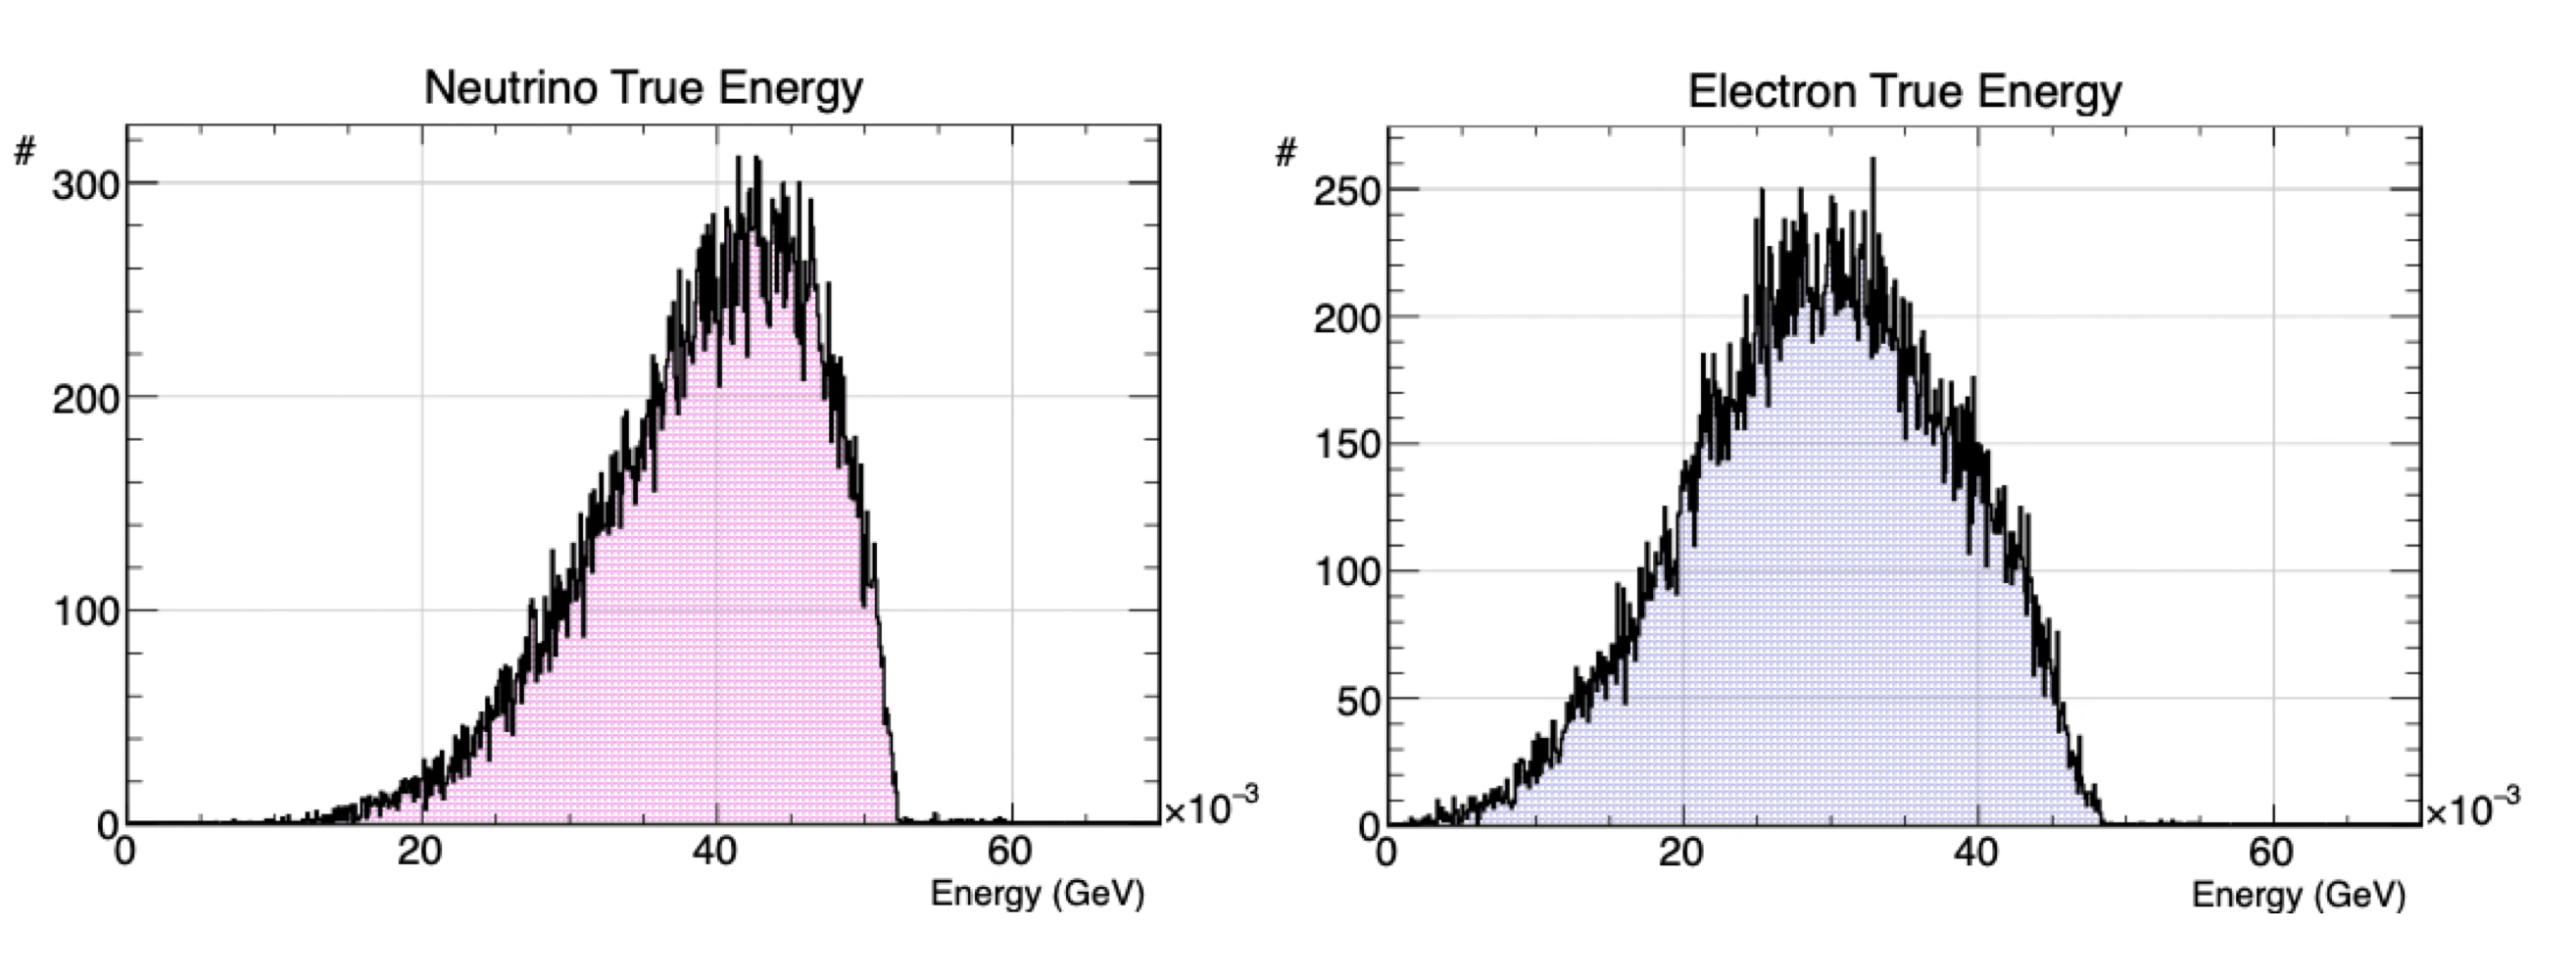
\includegraphics[width=160mm]{Figures/NuMI_muDAR_Neutrino_Electron_Energy.jpeg}
    \caption[Energy Distribution of Simulated $\mu$DAR $\nu_e$s from the NuMI Beam in MicroBooNE and the Electrons Produced in the Interaction]{{\textbf{Energy Distribution of Simulated $\mu$DAR $\nu_e$s from the NuMI Beam in MicroBooNE and the Electrons Produced in the Interaction}}\\}
    \label{sim_energy_dist_figures}
\end{figure}

\begin{figure}[h!]
    \centering
    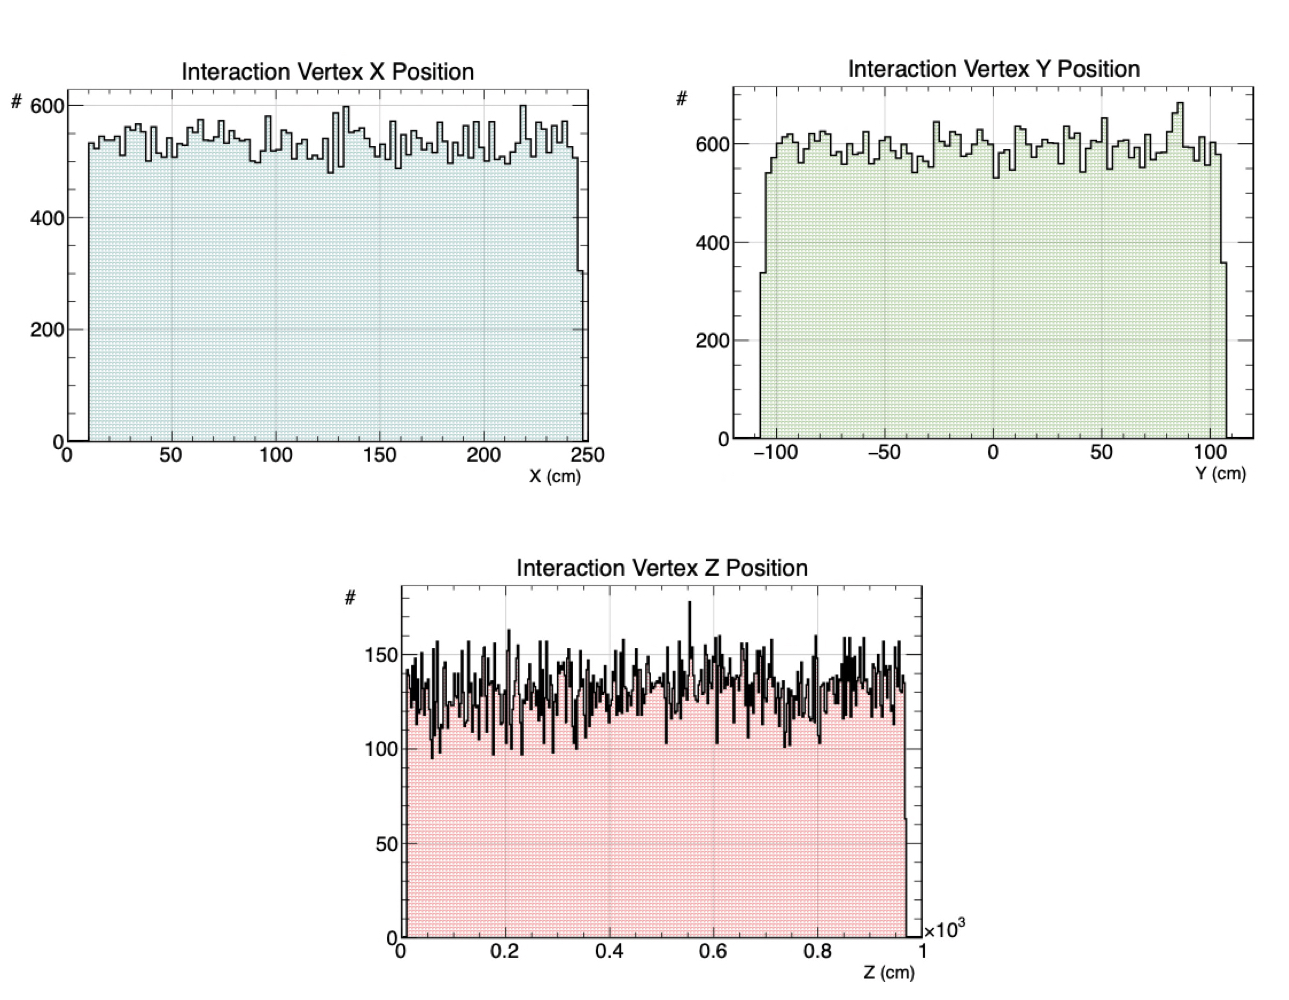
\includegraphics[width=160mm]{Figures/NuMI_muDAR_vertex.jpeg}
    \caption[Interaction Vertex Distribution of Simulated NuMI $\mu$DAR $\nu_e$s using MARLEY]{{\textbf{Interaction Vertex distribution of Simulated NuMI $\mu$DAR $\nu_e$s using MARLEY}}\\ .}
    \label{sim_vertex_dist_figures}
\end{figure}

\newpage
\section{Reconstruction of $\mu$DAR Events in MicroBooNE}

To reconstruct the events in MicroBooNE, we count on a chain of reconstruction software that processes the signal, carries it through a low level event reconstruction, up to higher level event reconstruction. In MicroBooNE, all of those are done using reconstruction algorithms that are part of LArSoft. To name the chain we used for this analysis: the signal is processed through a signal noise filter, a deconvolution algorithm, a hit finding algorithm, and the blip reconstruction algorithm (that handles two steps: cluster finding and plane matching). I will go over what each of those steps do in this chapter, and how the final algorithm performs in the Monte Carlo simulation.  

\subsection{Signal Processing}

Once the detector captures the signals presented in figure \ref{uboone_digital_signal}, we need to convert this raw signal into usable information. 
Initially, the wires record any measured voltage as a function of time in the LArTPC during the readout window, which means it will include a lot of noise from various sources. Therefore, our first step is to pass the raw data through a noise filter algorithm. Deatils on it can be found on paper \cite{noise_filter}. You can see an example of the filters performance in figure \ref{noise_filter}. 

\begin{figure}[h!]
    \centering
    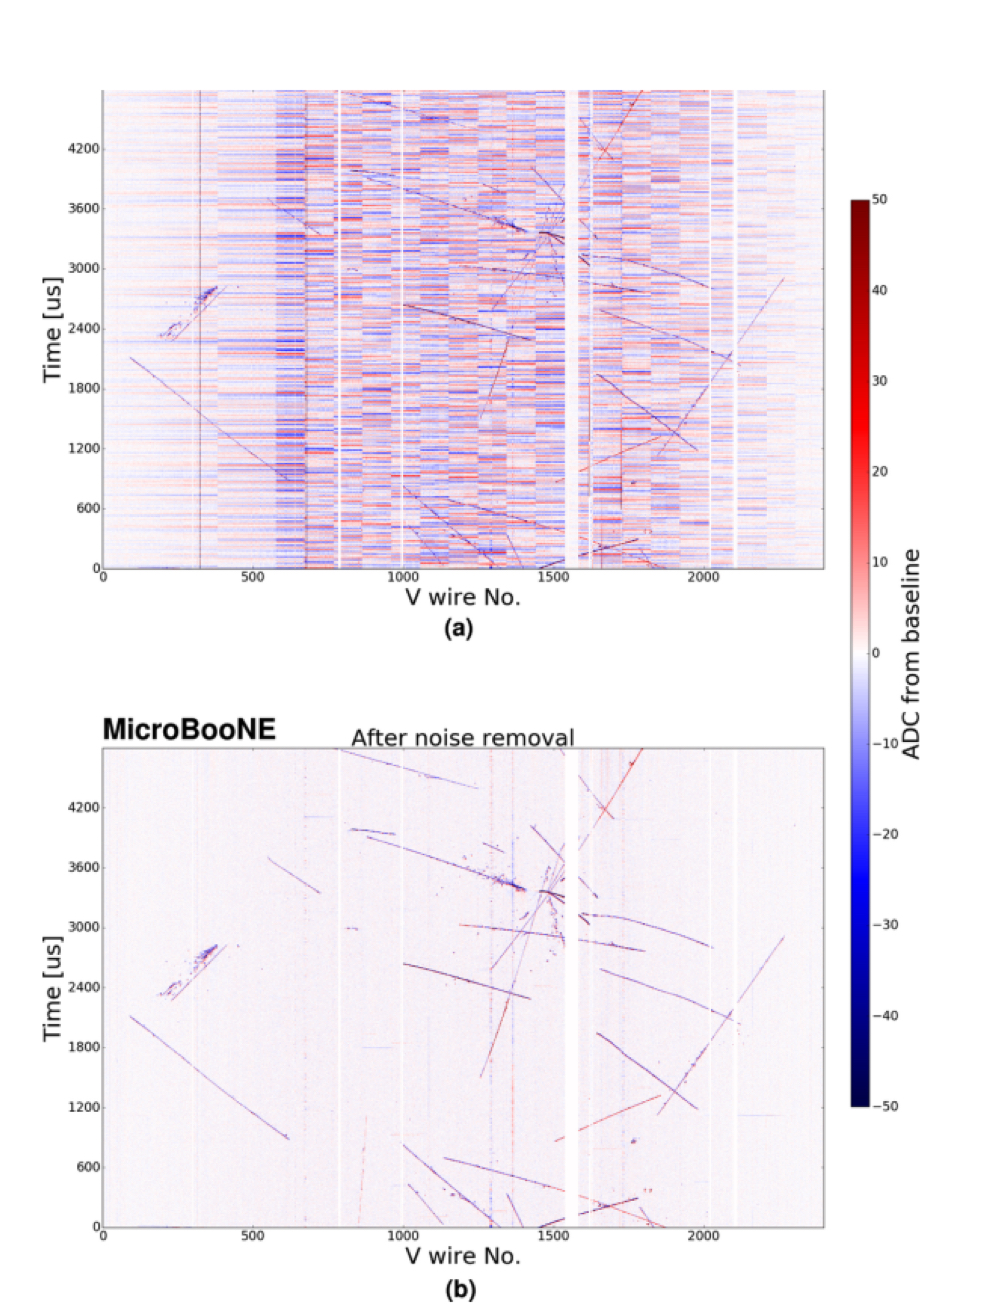
\includegraphics[width=100mm]{Figures/noise_removal.jpeg}
    \caption[MicroBooNE Software Noise Filter Performance]{{\textbf{MicroBooNE Software Noise Filter Performance}}\\ A 2D event display of the V plane from MicroBooNE data run $3493$, event $41075$ showing the raw signal (a) before and (b) after noise filtering. A clean event signature is recovered once all the identified noise sources are subtracted \cite{noise_filter}.}
    \label{noise_filter}
\end{figure}

After removing the excess noise, we need to extract the drift electron distribution from the TPC wire signals from the waveforms. The way to do this is to pass them through a 2D deconvolution procedure based on Fast Fourier Transform. This procedure suffers from low-frequency noise on the two induction planes due to the bipolar shape of the measured signals. We solve this by only considering regions of interest (ROI) on the waveforms just large enough to cover the signal. Anything that is not inside the ROI is discarded. The ROI procedure is also performed in the collection plane to reduce the data stored. The final result from this signal processing is a deconvolved wire waveform, in which a single individual element of charge signal takes the form of a Gaussian function. On figure \ref{noise_deconv} you can see the impact of each of those steps on the data. A more detailed description of MicroBooNE's signal processing is available at \cite{signal_proc}. 

\begin{figure}[h!]
    \centering
    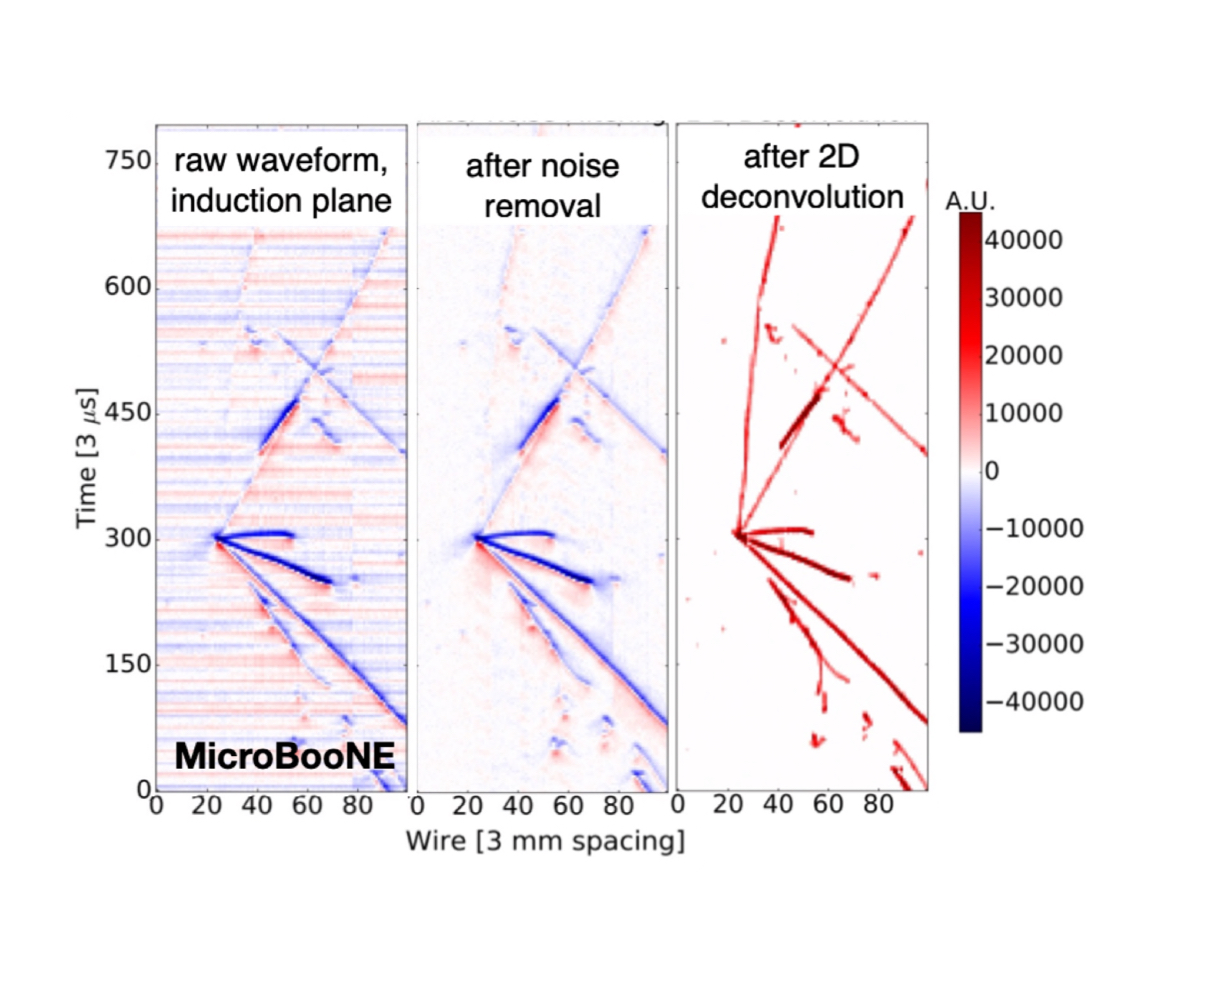
\includegraphics[width=120mm]{Figures/noise_deconv.jpeg}
    \caption[MicroBooNE Signal Processing Steps and Impact on Data]{{\textbf{MicroBooNE Signal Processing Steps and Impact on Data}}\\ 2D event displays of the U plane from MicroBooNE data run $3493$, event $41075$, zoomed in on a neutrino interaction candidate. The left-most image shows the raw digitized waveform in units of average baseline-subtracted analog-to-digital converter (ADC) scaled by $250$ per $3$ $\mu$s. The next panel shows the image after the noise removal algorithm, again in units of average baseline-subtracted ADC scaled by $250$ per $3$ $\mu$s. The last panel shows the image after processing with 2D deconvolution, also in units of electrons per $3$ $\mu$s. Adapted from \cite{Lauren_thesis}.}
    \label{noise_deconv}
\end{figure}

\subsection{Hit Finding}

The first low level reconstruction done in the signal is the ``hit finding". In it, the wire waveforms are scanned and, in case its local maxima is above a given threshold, the signal is fit into a Gaussian curve and called a ``hit". The curve's height, area, and peak time are recorded. The number of electrons detected by the wire is proportional to the area of the hit \cite{avinay_thesis}.

\subsection{Pandora}

Pandora is the multi-algorithm pattern recognition framework used by MicroBooNE to identify and reconstruct tracks in the LArTPC. It takes in the hits information in each plane and combines them to build three 2D images. Assuming the drift (x) direction is common among them, Pandora combines the different views and forms a 3D reconstruction. Beyond that, Pandora uses pattern recognition to identify the topology of the events. In a first step, Pandora tags cosmic muons and removes the associated hits. Once we have a cosmic-muons-free hit collection, Pandora works by identifying neutrino interaction vertices and reconstructing tracks and showers from it. You can see an example of a simulated neutrino interaction reconstructed using Pandora in \ref{pandora}. More information on the Pandora algorithms' use in MicroBooNE can be found in the paper \cite{pandora}.

Although Pandora is optimized to reconstruct tracks, it is not developed to identify smaller, blip-like depositions characteristic of the MeV-scale neutrino interactions. In this work, we use a combination of Pandora and Blip Reconstruction algorithms to identify the $\mu$DAR neutrino candidates. 

\begin{figure}[h!]
    \centering
    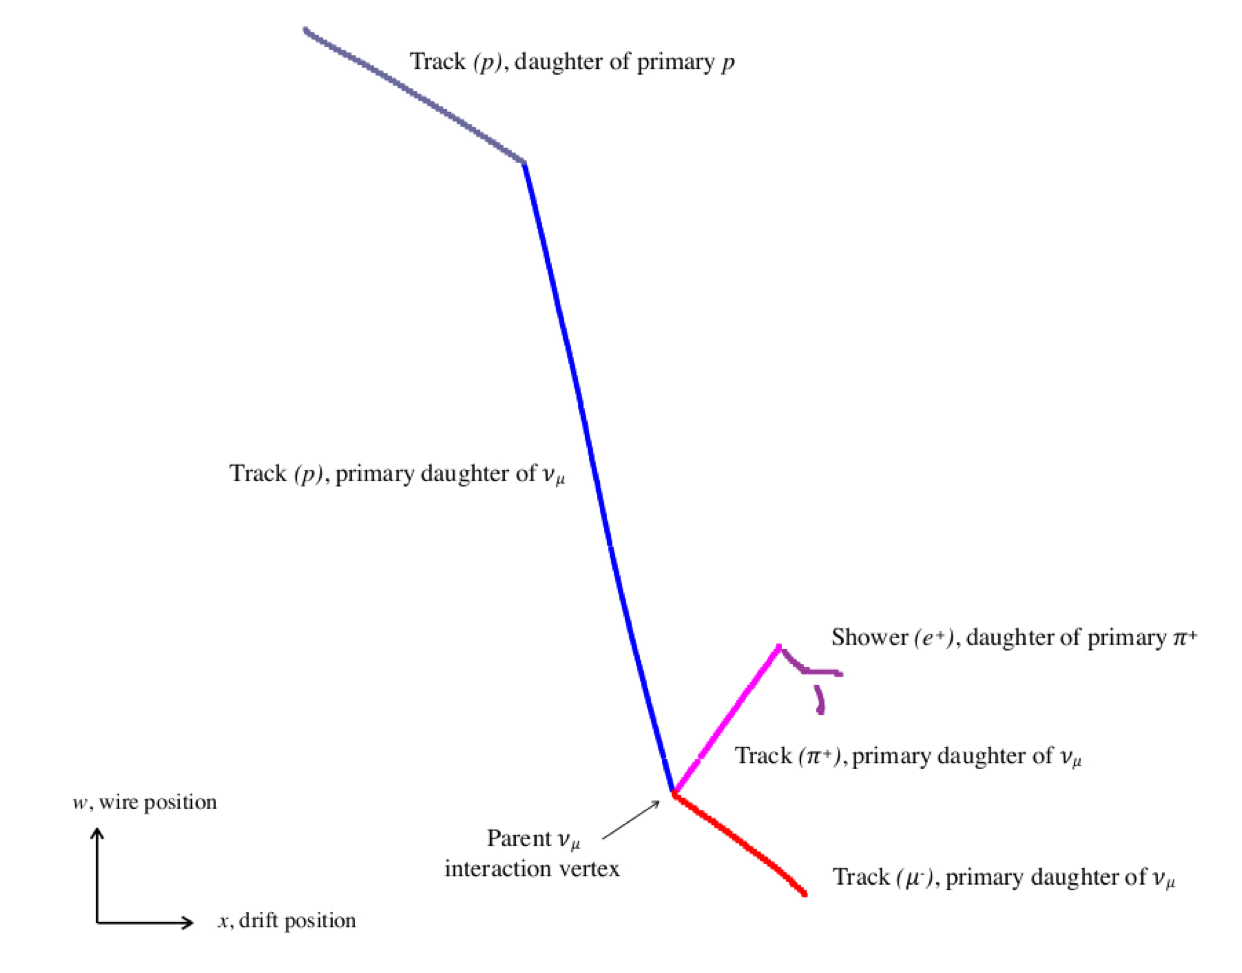
\includegraphics[width=110mm]{Figures/pandora.jpeg}
    \caption[Simulated Neutrino Interaction Reconstructed Using Pandora]{{\textbf{Simulated Neutrino Interaction Reconstructed Using Pandora}}\\ Illustration of the Pandora recontruction of a simulated charged current $\nu_{\mu}$ interaction in MicroBooNE and its products. The interaction includes a muon, proton and charged pion in the visible final state \cite{pandora}.}
    \label{pandora}
\end{figure}

\subsection{Blip Reconstruction}
The Blip Reconstruction is a class of algorithms that identifies MeV-scale charge depositions in the LArTPC and reconstructs them into 3D clusters. Due to their nature, those depositions resemble point-like signals, which we call ``blips". Their reconstruction is divided into two parts: the cluster finding and the plane matching. 

On cluster finding, the algorithm works to isolate groups of hits in each of the planes. It veto hits in or nearby a configurable distance of a Pandora-identified track. Figure \ref{blip_track_veto} illustrates that procedure. Next, it individually clusters the left-over hits in each wire plane. In our selection, we reject any tracks bigger than $25$ cm, as that is the limit length of a $53$ MeV electron track. We also set the veto to reject any blips $20$ cm away tracks bigger than $15$ cm. 

\begin{figure}[h!]
    \centering
    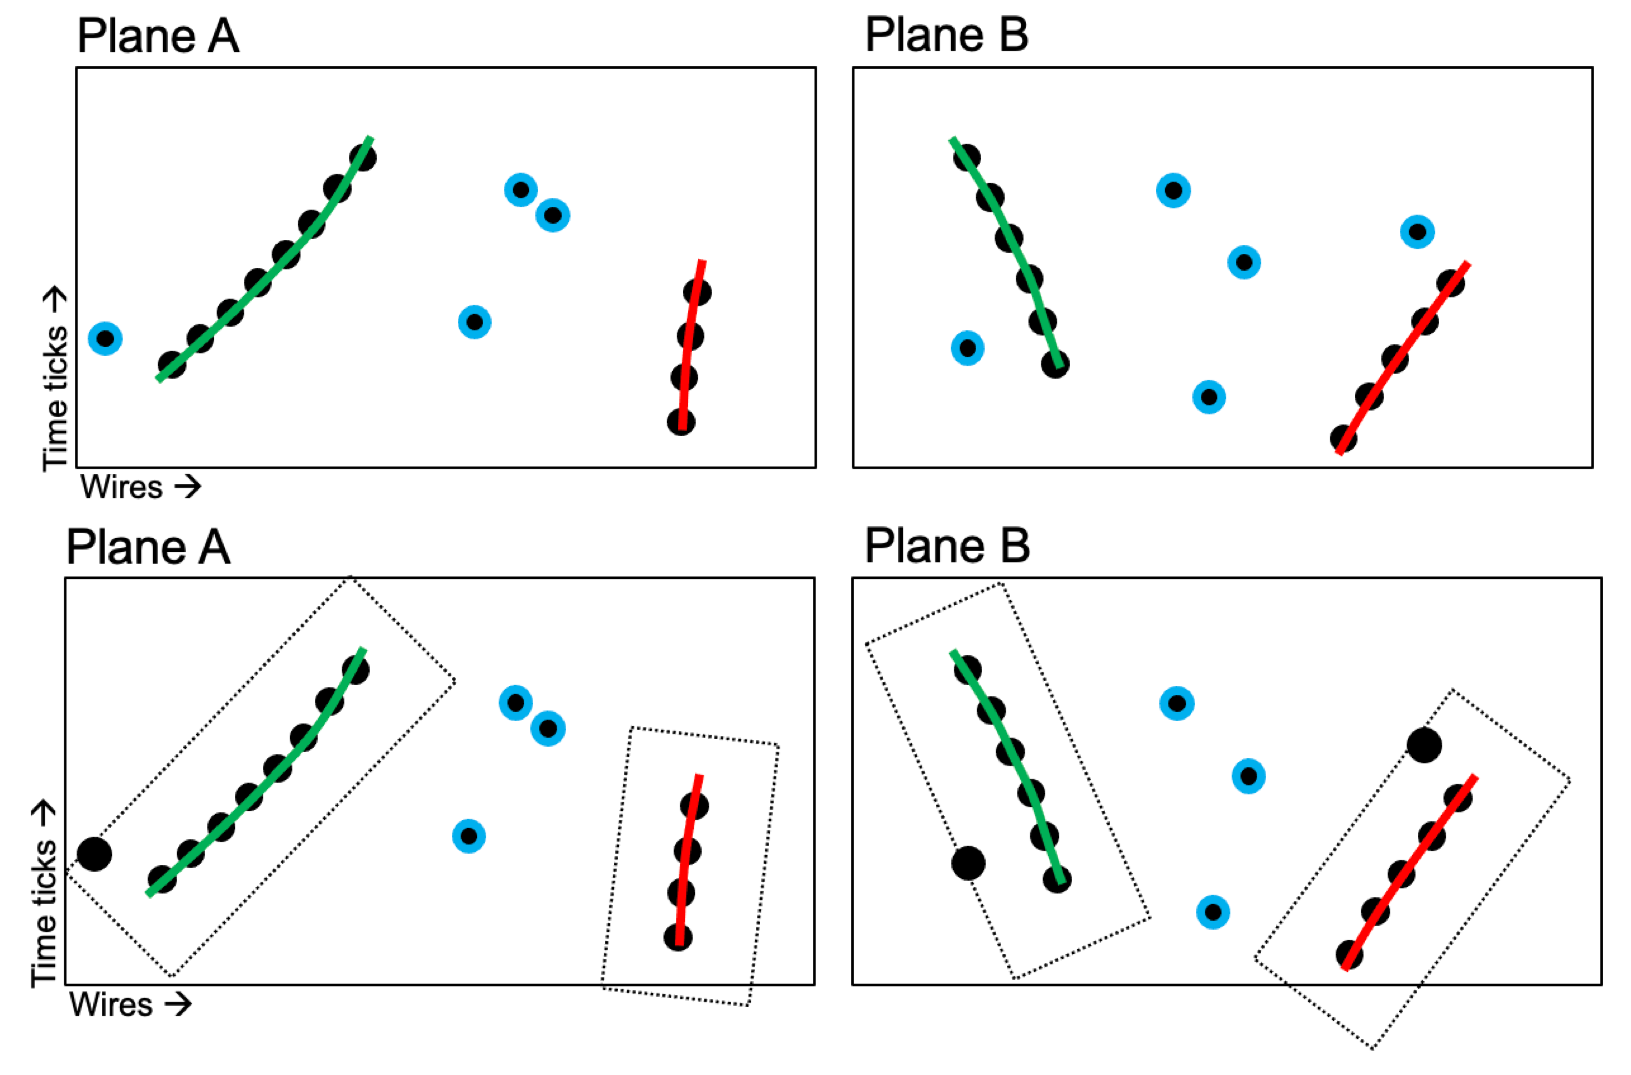
\includegraphics[width=110mm]{Figures/blip_track_veto.png}
    \caption[BlipReco - Pandora Track Hit Veto]{{\textbf{BlipReco - Pandora Track Hit Veto}}\\ In a first step, BlipReco veto all hits in or near a Pandora-identified track. Adapted from \cite{will_CM_Aug}.}
    \label{blip_track_veto}
\end{figure}

Then, on plane matching, it finds matches between the clusters from different planes based on their overlapping in position and time (see figure \ref{plane-matching}). It is also required that the clusters are located in wires that cross. 

\begin{figure}[h!]
    \centering
    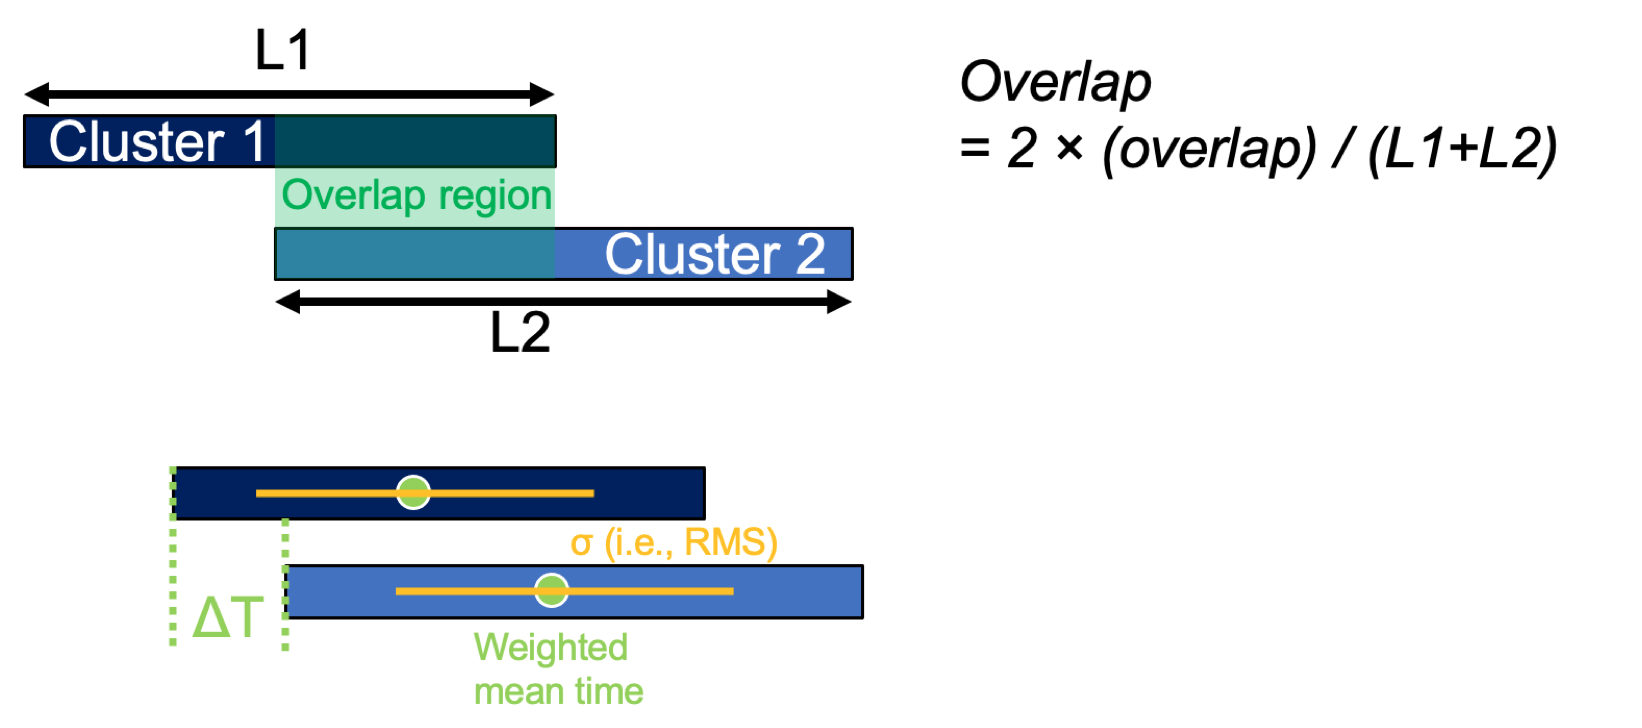
\includegraphics[width=120mm]{Figures/blip_cluster_match.png}
    \caption[BlipReco - Plane Matching]{{\textbf{BlipReco - Plane Matching}}\\ The BlipReco algorithm finds matches between clusters in different planes by comparing their time and position overlapping. Adapted from \cite{will_CM_Aug}.}
    \label{plane-matching}
\end{figure}

Then, the measured integrated charge in each plane must not differ by a configurable limit (the standard set in the code is $10^3$ e) \cite{will_CM_Aug}. In figure \ref{charge_match} you can see how the charge match is configured to only allow a certain deviation from the diagonal in a Charge in Cluster in Plane 1 versus Charge in a Cluster in Plane 2 plot.

\begin{figure}[h!]
    \centering
    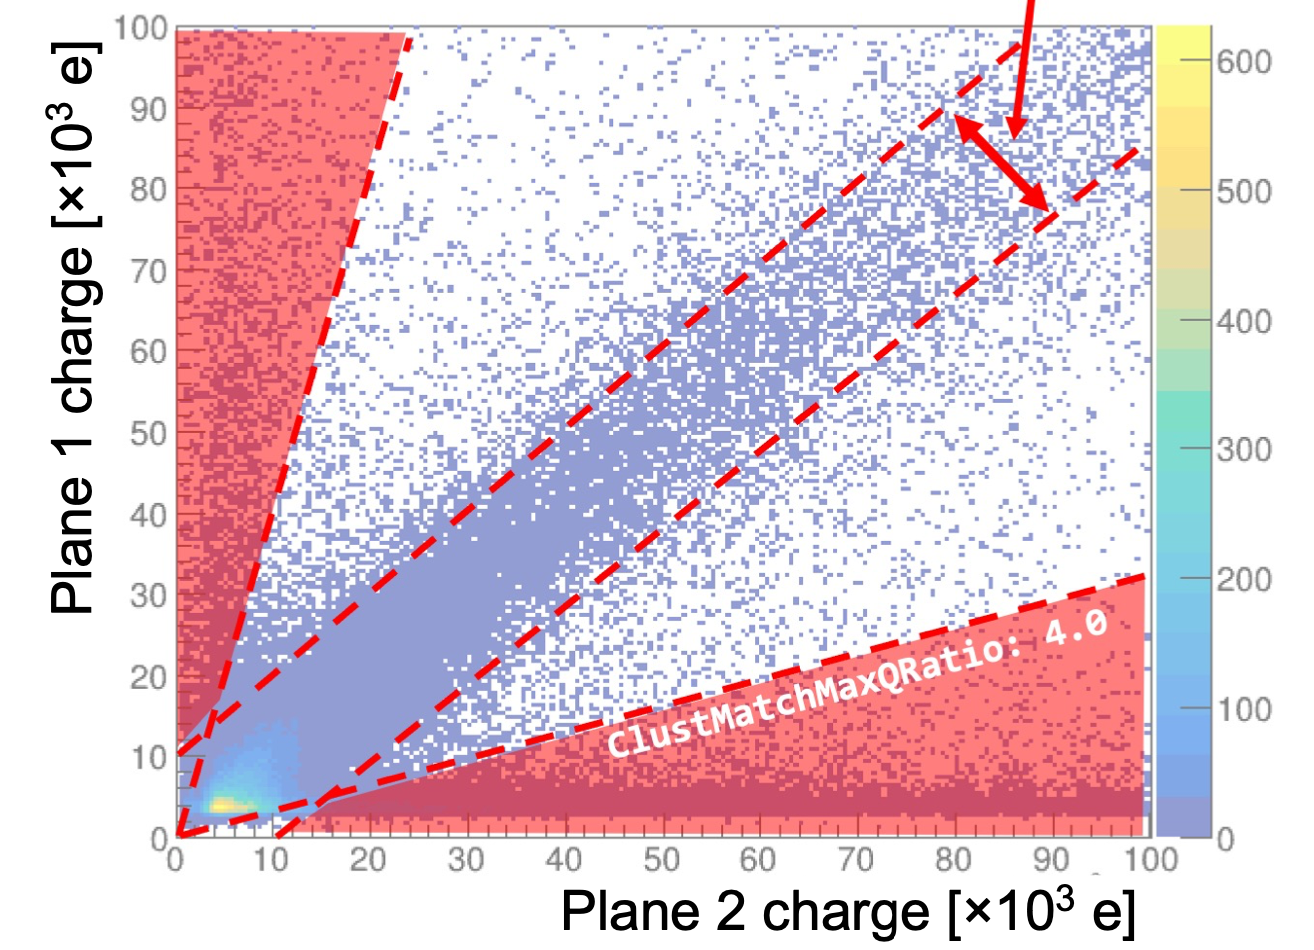
\includegraphics[width=100mm]{Figures/blip_charge_match.png}
    \caption[BlipReco - Cluster Charge Match]{{\textbf{BlipReco - Cluster Charge Match}}\\ In a last step, the BlipReco code tries to best match the integrated charge in clusters \cite{will_CM_Aug}. The red arrow points to the margin of divergence from the diagonal, allowed to consider the charge in different clusters a match. }
    \label{charge_match}
\end{figure}

Lastly, it does the energy and position reconstruction. The energy (E) is computed based on the charge (Q) collected following the expression:
\begin{equation}
    E=Q\times R^{-1} \times (24)
\end{equation}

Where R is the electron recombination factor in MicroBooNE and $24$ eV is the average energy required to ionize LAr \cite{lariat_calorimetry_lar}. 

For the position, the 3D position is reconstructed as shown in figure \ref{blip_position}. 

\begin{figure}[h!]
    \centering
    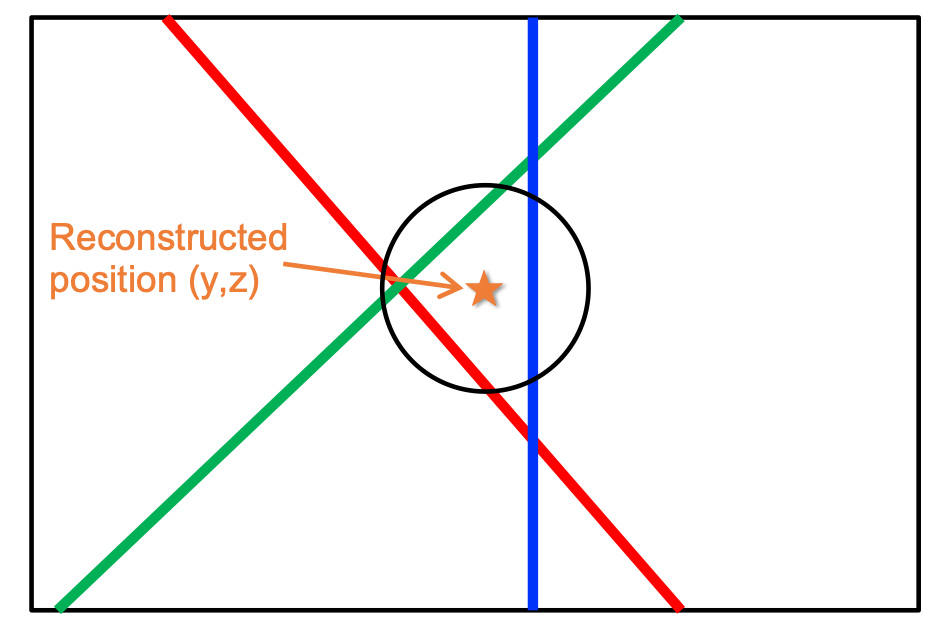
\includegraphics[width=90mm]{Figures/blip_reco_position.png}
    \caption[BlipReco - Position Reconstruction]{{\textbf{BlipReco - Position Reconstruction}}\\ The reconstruction of the position is based on the overlaping position in which the wires cross \cite{will_CM_Aug}.}
    \label{blip_position}
\end{figure}

\section{Data Analysis}
As established on the previous sessions, our $\mu$DAR $\nu_e$ candidate events are composed by a main electron, of energy between $20$ to $50$ MeV, and dexcitation photons around it. In figures \ref{signal_evd_1}, \ref{signal_evd_2}, and \ref{signal_evd_3} you can see the event display for a few simulated MARLEY signal events. 

\begin{figure}[h!]
    \centering
    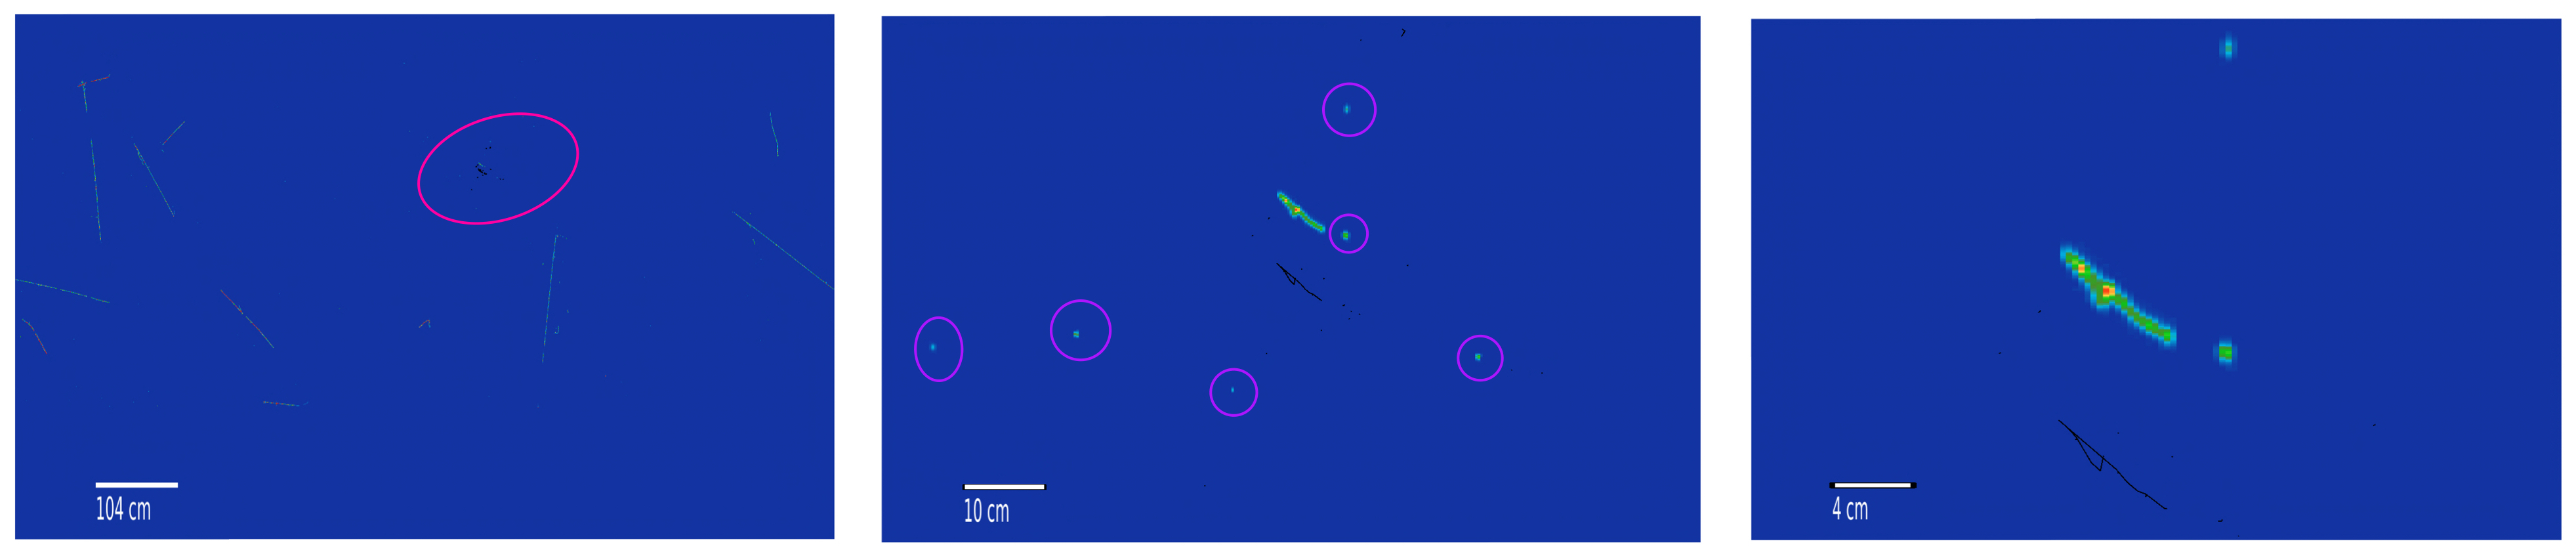
\includegraphics[width=200mm]{Figures/signal_evd_1.jpeg}
    \caption[Event display of MARLEY simulated $\mu$DAR $\nu_e$s in MicroBooNE]{{\textbf{Event display of MARLEY simulated $\mu$DAR $\nu_e$s in MicroBooNE}}\\ Event display of MARLEY simulated $\mu$DAR $\nu_e$s in MicroBooNE. From left to right, frames of the same event zoomed in. In the left one, the full event display. In the middle, its possible to see the main electron and the deexcitation photons, marked in purple. In the left, the main electron. The black shadows are the MC true information, whether the the blue-green-red are reconstructed information.}
    \label{signal_evd_1}
\end{figure}

\begin{figure}[h!]
    \centering
    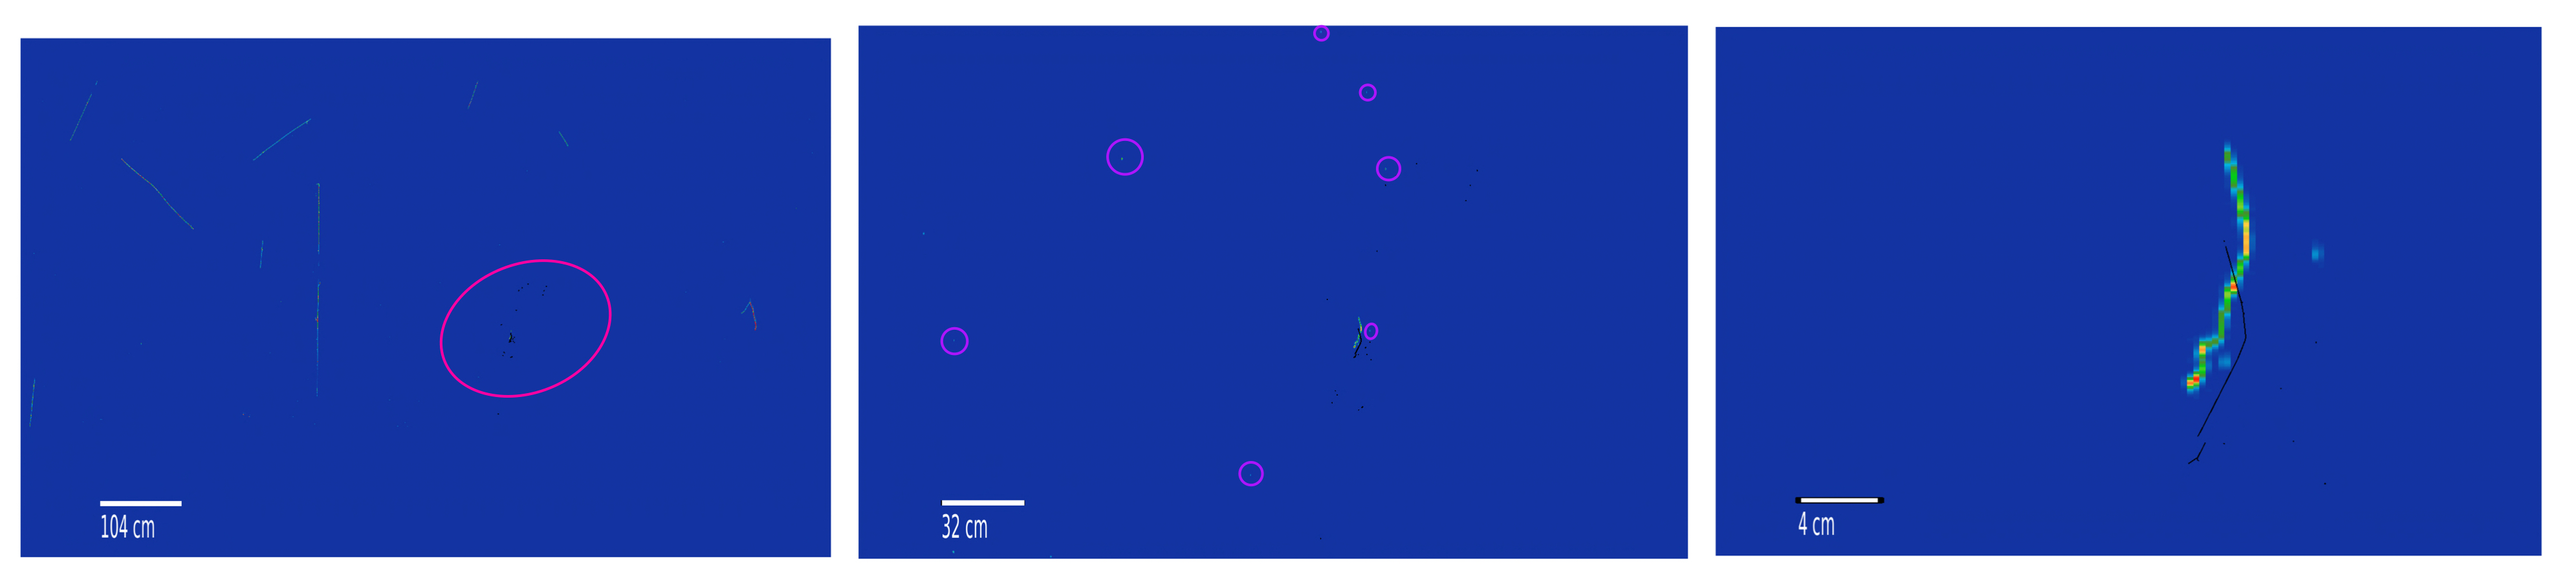
\includegraphics[width=200mm]{Figures/signal_evd_2.jpeg}
    \caption[Event display of MARLEY simulated $\mu$DAR $\nu_e$s in MicroBooNE]{{\textbf{Event display of MARLEY simulated $\mu$DAR $\nu_e$s in MicroBooNE}}\\ Event display of MARLEY simulated $\mu$DAR $\nu_e$s in MicroBooNE. From left to right, frames of the same event zoomed in. In the left one, the full event display. In the middle, its possible to see the main electron and the deexcitation photons, marked in purple. In the left, the main electron. The black shadows are the MC true information, whether the the blue-green-red are reconstructed information.}
    \label{signal_evd_2}
\end{figure}

\begin{figure}[h!]
    \centering
    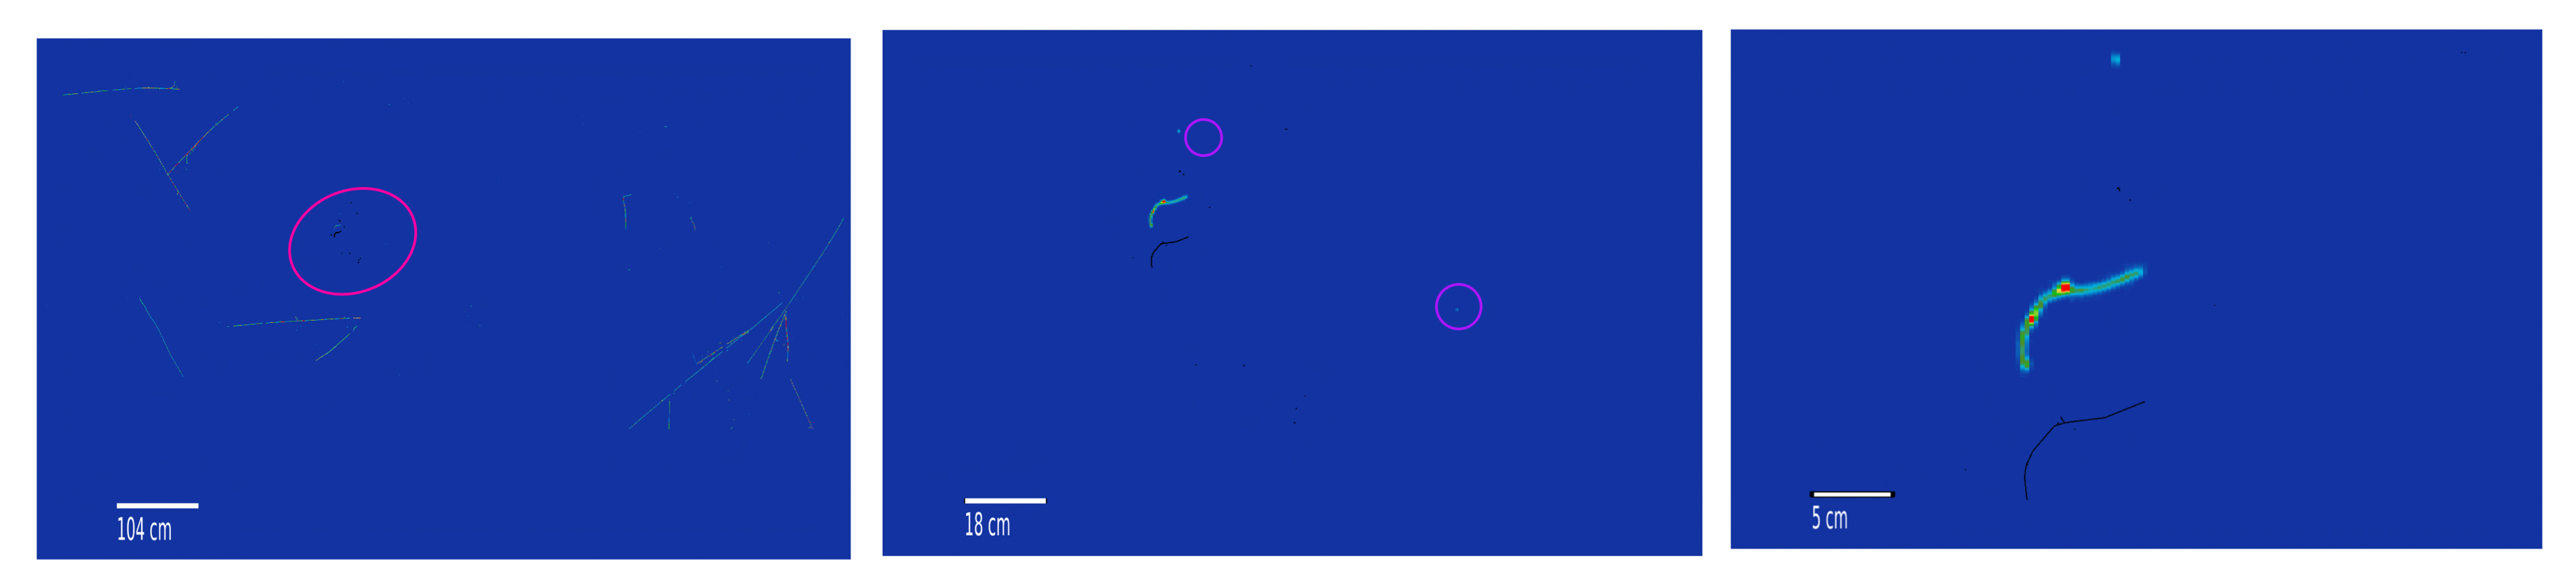
\includegraphics[width=200mm]{Figures/signal_evd_3.jpeg}
    \caption[Event display of MARLEY simulated $\mu$DAR $\nu_e$s in MicroBooNE]{{\textbf{Event display of MARLEY simulated $\mu$DAR $\nu_e$s in MicroBooNE}}\\ Event display of MARLEY simulated $\mu$DAR $\nu_e$s in MicroBooNE. From left to right, frames of the same event zoomed in. In the left one, the full event display. In the middle, its possible to see the main electron and the deexcitation photons, marked in purple. In the left, the main electron. The black shadows are the MC true information, whether the the blue-green-red are reconstructed information.}
    \label{signal_evd_3}
\end{figure}

As a first approach, this analysis focus on identifying the main electrons from the $\mu$DAR-LAr interaction. 
There are a number of background events that can mimic our main electron candidates, such as particles from higher energy $\nu_e$s and $\nu_{\mu}$s, cosmic rays, and delta-rays and Bremsstrahlung. In figures \ref{bkg_evd_1},\ref{bkg_evd_2}, and \ref{bkg_evd_3}  you can see the event display of background events from GENIE MC and from data overlay cosmics. 

\begin{figure}[h!]
    \centering
    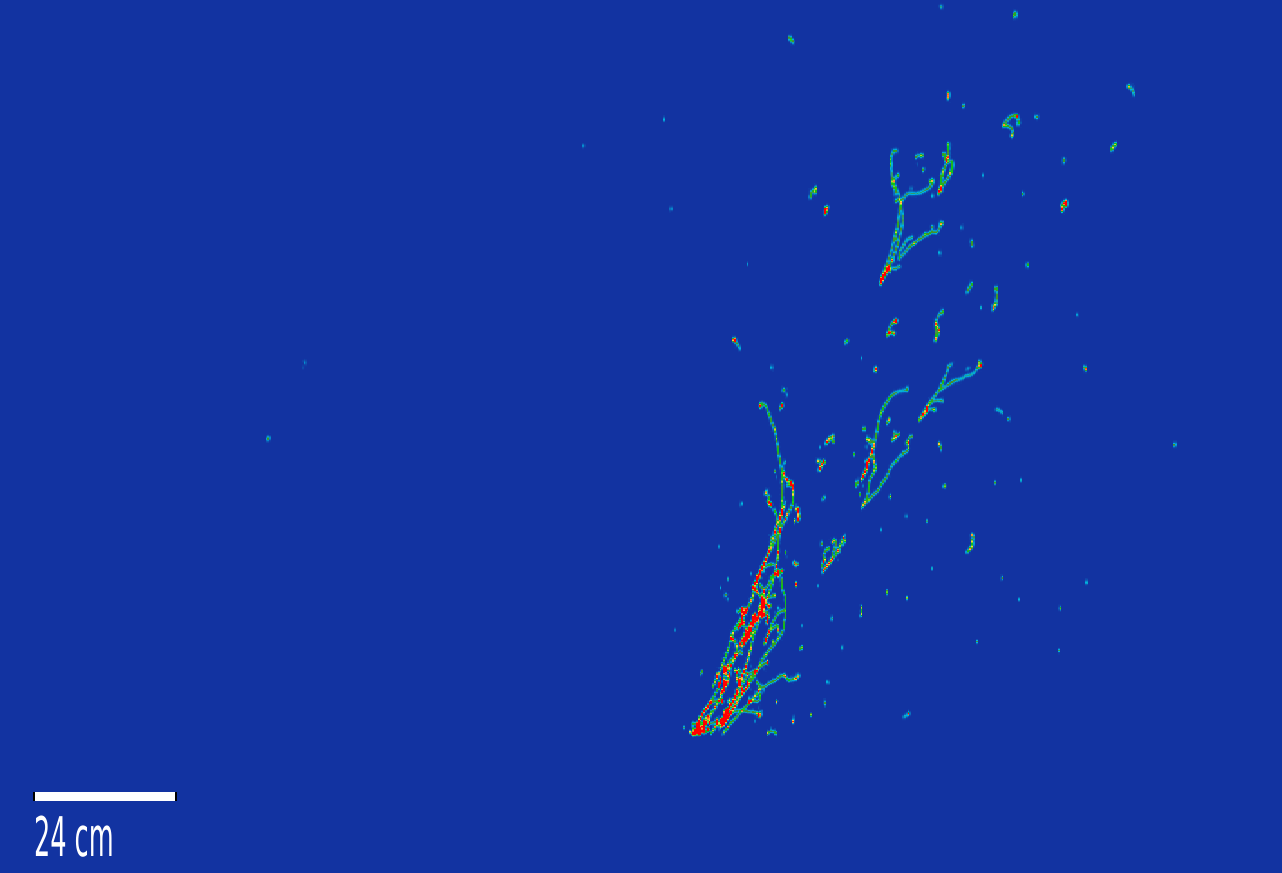
\includegraphics[width=90mm]{Figures/shower_evd_1.png}
    \caption[Event display of a background from the GENIE $\nu_{mu}$ simulated events in MicroBooNE.]{{\textbf{Event display of a background from the GENIE $\nu_{mu}$ simulated events in MicroBooNE.}}\\ this is a caption}
    \label{bkg_evd_1}
\end{figure}

\begin{figure}[h!]
    \centering
    \includegraphics[width=120mm]{Figures/numu_evd.jpeg}
    \caption[Event display of a background from the GENIE $\nu_{\mu}$ simulated event in MicroBooNE.]{{\textbf{Event display of a background from the GENIE $\nu_{\mu}$ simulated events in MicroBooNE.}}\\ this is a caption}
    \label{bkg_evd_2}
\end{figure}

\begin{figure}[h!]
    \centering
    \includegraphics[width=90mm]{Figures/shower_evd_2.png}
    \caption[Event display of a background from the GENIE $\nu_{\mu}$ simulated events in MicroBooNE.]{{\textbf{Event display of an electromagneticshower background found in the GENIE $\nu_{e}$ simulated events in MicroBooNE.}}\\ this is a caption}
    \label{bkg_evd_3}
\end{figure}


\subsubsection{$\mu$DAR events Truth versus Reco Comparitions}

To evaluate the performance of the blip reconstruction algorithm in the $\mu$DAR $\nu_e$ events, it is conviniente to plot reco versus true for the variables evaluated. You can see in figures \ref{reco_vs_true_energy}, \ref{reco_vs_true_vertex_x}, \ref{reco_vs_true_vertex_y}, and \ref{reco_vs_true_vertex_z} how the blip reconstruction tool performes for energy and vertex X, Y and Z positions.

\begin{figure}[h!]
    \centering
    \includegraphics[width=120mm]{Figures/energy_reco_vs_true.pdf}
    \caption[Energy reconstruction performance in MARLEY $\nu_e$ main electron events]{{\textbf{Energy reconstruction performance in MARLEY $\nu_e$ main electrons}}\\ Reconstructed energy versus true energy for simulated MARLEY $\nu_e$ electrons. Although the majority of the population is located at the diagonal, there is a clear deficit in the reconstructed events for a non-negligible amount of the candidates.}
    \label{reco_vs_true_energy}
\end{figure}

\begin{figure}[h!]
    \centering
    \includegraphics[width=120mm]{Figures/x_reco_vs_true.pdf}
    \caption[Vertex X position reconstruction performance in MARLEY $\nu_e$ main electron events]{{\textbf{Vertex X position reconstruction performance in MARLEY $\nu_e$ main electron events}}\\ Reconstructed vertex X versus true vertex X for simulated MARLEY $\nu_e$ electrons. Almost all candidates fall into the diagonal of the canvas, indicating that the reconstruction tools perform well in this sample.}
    \label{reco_vs_true_vertex_x}
\end{figure}

\begin{figure}[h!]
    \centering
    \includegraphics[width=120mm]{Figures/y_reco_vs_true.pdf}
    \caption[Vertex Y position reconstruction performance in MARLEY $\nu_e$ main electron events]{{\textbf{Vertex Y position reconstruction performance in MARLEY $\nu_e$ main electron events}}\\ Reconstructed vertex Y versus true vertex Y for simulated MARLEY $\nu_e$ electrons. Almost all candidates fall into the diagonal of the canvas, indicating that the reconstruction tools perform well in this sample.}
    \label{reco_vs_true_vertex_y}
\end{figure}

\begin{figure}[h!]
    \centering
    \includegraphics[width=120mm]{Figures/z_reco_vs_true.pdf}
    \caption[Vertex Z position reconstruction performance in MARLEY $\nu_e$ main electron events]{{\textbf{Vertex Z position reconstruction performance in MARLEY $\nu_e$ main electron events}}\\ Reconstructed vertex Z versus true vertex Z for simulated MARLEY $\nu_e$ electrons. Almost all candidates fall into the diagonal of the canvas, indicating that the reconstruction tools perform well in this sample.}
    \label{reco_vs_true_vertex_z}
\end{figure}

To thoroughly evaluate the background and make an informed choice on cuts for the selection, we used three different simulated MC (GENIE $\nu_{\mu}$, GENIE $\nu_{e}$, and MARLEY) and EXT NuMI data. In the GENIE $\nu_{\mu}$, we have simulated $\nu_{\mu}$ events overlayed with EXT unbiased data. In the GENIE $\nu_{e}$, we have simulated $\nu_{e}$ events overlayed with EXT unbiased data. In the MARLEY, we have simulated $\mu$DAR $\nu_e$ events overlayed with EXT unbiased data. We evaluate the background contribution of true simulated events and the overlayed cosmic rays for each MC sample. Each must be evaluated individually because of the different neutrino contributions in the beam and cosmic rays. The background is broken into its five contributions: from EXT cosmic rays, from GENIE $\nu_{e}$, from GENIE $\nu_{mu}$, from GENIE $\nu_{e}$ cosmic rays, and from GENIE $\nu_{mu}$ cosmic rays. 

The first cut applied in the selection to reject background is the fiducial volume cut to reject blips in our selection. Blips closer to the corners of the detector are more likely to be from cosmic rays and therefore are rejected, as shown in figures \ref{vertex_X},\ref{vertex_Y}, and \ref{vertex_Z}. The reconstructed blip position corresponds to the middle of the track. 

\begin{figure}[h!]
    \centering
    \includegraphics[width=120mm]{Figures/vertex_X.pdf}
    \caption[Reconstructed Blip X Position.]{{\textbf{Reconstructed Blip X Position.}}\\ Distribution of reconstructed blip X position for MARLEY simulated events, overlay cosmic-rays, Overlay GENIE $\nu_{mu}$,and Overlay GENIE $\nu_{e}$. The vertical gray lines mark the acceptance cuts on the event selection. All the events below the left mark or after the right mark were rejected.}
    \label{vertex_X}
\end{figure}

\begin{figure}[h!]
    \centering
    \includegraphics[width=120mm]{Figures/vertex_Y.pdf}
    \caption[Reconstructed Blip Y Position.]{{\textbf{Reconstructed Blip Y Position.}}\\ Distribution of reconstructed blip Y position for MARLEY simulated events, overlay cosmic-rays, Overlay GENIE $\nu_{mu}$,and Overlay GENIE $\nu_{e}$. The vertical gray lines mark the acceptance cuts on the event selection. All the events below the left mark or after the right mark were rejected.}
    \label{vertex_Y}
\end{figure}

\begin{figure}[h!]
    \centering
    \includegraphics[width=120mm]{Figures/vertex_Z.pdf}
    \caption[Reconstructed Blip Z Position.]{{\textbf{Reconstructed Blip Z Position.}}\\ Distribution of reconstructed blip Z position for MARLEY simulated events, overlay cosmic-rays, Overlay GENIE $\nu_{mu}$,and Overlay GENIE $\nu_{e}$. The vertical gray lines mark the acceptance cuts on the event selection. All the events below the left mark or after the right mark were rejected.}
    \label{vertex_Z}
\end{figure}

Next, we only accept blips with reconstructed energy, $20 <$ E$_{reco}$ $< 53$ MeV, bigger than $4$ cm, and that had a cluster match on all 3 planes of wires. The first two cuts are chosen based on the topology of the signal events, whether the last one is a data quality cut.
The distribution of those cuts for simulated signal and background can be seen in figures \ref{blip_size}, \ref{blip_energy}, and \ref{blip_nplanes}.

\begin{figure}[h!]
    \centering
    \includegraphics[width=120mm]{Figures/blip_size.pdf}
    \caption[Reconstructed Blip Size.]{{\textbf{Reconstructed Blip Size.}}\\ Distribution of reconstructed size for MARLEY simulated events, overlay cosmic-rays, Overlay GENIE $\nu_{mu}$,and Overlay GENIE $\nu_{e}$. The cuts applied are represented by the gray vertical lines.}
    \label{blip_size}
\end{figure}

\begin{figure}[h!]
    \centering
    \includegraphics[width=120mm]{Figures/Energy_MC.pdf}
    \caption[Reconstructed Energy.]{{\textbf{Reconstructed Energy.}}\\ Distribution of reconstructed energy for MARLEY simulated events, overlay cosmic-rays, Overlay GENIE $\nu_{mu}$,and Overlay GENIE $\nu_{e}$. The energy cut is represented by the vertical gray lines.}
    \label{blip_energy}
\end{figure}

\begin{figure}[h!]
    \centering
    \includegraphics[width=120mm]{Figures/blip_n_planes.pdf}
    \caption[Number of Planes Cluster-Matched.]{{\textbf{Number of Planes Cluster-Matched.}}\\ Distribution of number of planes cluster-matched for MARLEY simulated events, overlay cosmic-rays, Overlay GENIE $\nu_{mu}$,and Overlay GENIE $\nu_{e}$. It is required that there is a cluster-match between all the three planes. The cut is represented by the vertical gray line.}
    \label{blip_nplanes}
\end{figure}

In total, we are left with a total of 8776 selected background events, POT normalized to the amount of POT in NuMI Run1 data, and 1 selected signal events in MARLEY MC. Therefore, this work's selection purity computes to 0.011\%. The absolute numbers, the POT amounts in each sample, and the POT normalization can be found in \ref{bkg}. In the MARLEY $\nu_{e}$ MC sample we have a total of 30631 neutrinos interacting in the fiducial volume, and 2720 truth-matched candidates were selected. Therefore, our selection efficiency is of 8.88\%.

\begin{table}
    \centering
	\begin{tabular}{cccccc}
		\hline
		\textbf{Origin} & \textbf{Selected Events}	&	\textbf{POT in Sample}	&	\textbf{NuMI Run1 Beam On Data POT Limit} & \textbf{POT normalization Factor} & \textbf{Selected Events Data POT Normalized}\\
		\toprule
		MARLEY Signal & 2720 & 5.7437823 $\times 10^{23}$ & 2 $\times 10^{20}$ & 3.48 $\times 10^{-4}$ & 0.95 \\ 
		MARLEY Cosmic Ray & 1933 & 5.7437823 $\times 10^{23}$ & 2 $\times 10^{20}$ & 3.48 $\times 10^{-4}$ & 0.67 \\
		GENIE  $\nu_{\mu}$ Cosmic Ray &  2090  &  1.05669 $\times 10^{21}$  &  2 $\times 10^{20}$ &  1.89 $\times 10^{-1}$ & 1114.23 \\ 
        GENIE  $\nu_{\mu}$ & 5887 & 1.05669 $\times 10^{21}$ & 2 $\times 10^{20}$ & 1.89 $\times 10^{-1}$ & 395.58 \\
        GENIE  $\nu_{e}$ Cosmic Ray & 10471 & 8.11503 $\times 10^{22}$ & 2 $\times 10^{20}$ & 2.47$\times 10^{-3}$ & 25.81 \\
        GENIE  $\nu_{e}$ & 13095 & 8.11503 $\times 10^{22}$ & 2 $\times 10^{20}$ & 2.47$\times 10^{-3}$ & 32.27 \\
        EXT & 12586 & 9.19923274 $\times 10^{6}$ & 5.268051 $\times 10^{6}$ & 5.73 $\times 10^{-1}$ & 7207.52 \\
		\hline
	\end{tabular}
	\caption[Selection Background Evaluation]{{\textbf{Selection Background Evaluation Broken by Origin}}}
    \label{bkg}
\end{table}

\subsection{Data- Monte Carlo agreement}
When looking at the MC-data agreement for electron energy and track size in figures \ref{} and \ref{}, we can see a very good agreement. This is due to the fact that this analysis is dominated by cosmic ray background.

\begin{figure}[h!]
    \centering
    \includegraphics[width=120mm]{Figures/energy.pdf}
    \caption[Blip Energy Distribution for Selected Data Candidates, Simulated Background, and EXT.]{{\textbf{Blip Energy Distribution for Selected Data Candidates, Simulated Background, and EXT.}}\\ Distribution of blip energy reconstruction for NuMI Run1 Beam ON data, GENIE Overlay $\nu_{\mu}$, GENIE Overlay $\nu_{e}$, and EXT. The contribution of each of the background is stacked.}
    \label{blip_nplanes_data}
\end{figure}

\begin{figure}[h!]
    \centering
    \includegraphics[width=120mm]{Figures/size.pdf}
    \caption[Blip Size Distribution for Selected Data Candidates, Simulated Background, and EXT.]{{\textbf{Blip Size Distribution for Selected Data Candidates, Simulated Background, and EXT.}}\\ Distribution of blip size reconstruction for NuMI Run1 Beam ON data, GENIE Overlay $\nu_{\mu}$, GENIE Overlay $\nu_{e}$, and EXT. The contribution of each of the background is stacked.}
    \label{blip_size_data}
\end{figure}

\subsection{Sensitivity to nuclear structure theoretical models}

\section{Conclusion}


\chapter{Short Baseline Neutrino Detector's (SBND) Anode Plane Assemblies (APA) Assembly and Installation}
\section{The SBND Detector}
\section{APA Quality Assurance (QA) and Quality Control (QC) Tests}
\section{APA Installation Procedures}
\section{Status}

\chapter{Novel LAr Purity Monitor Using Paul Traps}
\section{Purity Monitors for LArTPCs}
\subsection{Motivation}
\subsection{Current Methods}
\section{Paul Trap as a Purity Monitor}
\subsection{Concept and Design}
\subsection{Simulation}
\subsubsection{Leapfrog integration}
\subsubsection{Paul Trap in Vacuum}
\subsubsection{Paul Trap in Fluid at $T = 0$ K}
\subsubsection{Paul Trap in Fluid at $T \geqslant 0$ K}
\section{Conclusion and Next Steps}



% Apêndices
\appendix % Não deletar
\isappendixtrue % Não deletar
\renewcommand\chaptername{Appendix}

\chapter{An appendix title}
\lipsum[1-3]


%%%%%%%%%%%%%%%%%%%%%%%%%%%%%%%%%%%%%%%%%%%%%% EPÍLOGO %%%%%%%%%%%%%%%%%%%%%%%%%%%%%%%%%%%%%%%%%%%%
\bibliography{References}

\bibliographystyle{unsrt}

\begin{thebibliography}{10}

% Escreva um simples arquivo com referências ou insira  o .bbl
%[1]
\bibitem{griffiths} D. Griffiths, \textbf{Introduction to Elementary Particle Physics}. Second edition, Wiley-VCH Verlag GmbH \& Co. KGaA, Weinheim. ISBN 978-3-527-40601-2. 2008.

%[2]
\bibitem{nobel_leptons} K. V. L. Sarma, \textbf{Nobel Leptons}. arXiv:hep-ph/9512420. 1995.

%[3]
\bibitem{cowan_reines} C. L. Cowan, F. Reines, F. B. Harrison, H. W. Kruse, and A. D. McGuire. \textbf{Detection of the Free Neutrino: A Confirmation}. Science. 1956.

%[4]
\bibitem{Konopinski_Mahmoud} E. J. Konopinski, H. M. Mahmoud, \textbf{The Universal Fermi Interaction}. Phys. Rev. \textbf{92}. 1953.

%[5]
\bibitem{two_neutrinos} G. Danby, J-M. Gaillard, K. Goulianos, L. M . Lederman, N. Mistry, M. Schwartz, J. Steinberger, \textbf{Observation of high-energy neutrino reactions and the existence of two kinds of neutrinos.} Phys. Rev. Lett. \textbf{9}, 1, 36. 1962.

%[6]
\bibitem{the_story_of_the_neutrino} G. Rajasekaran, \textbf{The Story of the Neutrino}. arXiv:1606.08715. 2016.

%[7]
\bibitem{pontecorvo_1967} B. Pontecorvo, J. Exptl., \textbf{Neutrino Experiments and The Problem of Conservation of Leptonic Charge}. Theoret. Phys. \textbf{53}, 1717 (1967), Sov. Phys. JETP \textbf{26}, 984. 1968.

%[8]
\bibitem{neutrino_oscillations_brief_history_and_present_status} S. M. Bilenky, \textbf{Neutrino oscillations: brief history and present status}. arXiv:1408.2864. 2014.

%[9]
\bibitem{tau_neutrino_discovery}K. Kodama \textit{et al.}, \textbf{Observation of tau neutrino interactions}.Phys. Lett. B \textbf{504}, 218-224. 2001. 

%[10]
\bibitem{MNS} Z. Maki \textbf{et al.}, \textbf{Remarks on the Unified Model of Elementary Particles}. Prog. Theor. Phys. \textbf{28}, 870-880. 1962.

%[11]
\bibitem{PMNS} B. Pontecorvo, \textbf{Inverse beta processes and nonconservation of lepton charge}. Soviet Phys. JETP. \textbf{7}, 172. 1958.

%[12]
\bibitem{oscillation_math} C. Giunti, C. K. Kim, \textbf{Fundamentals of Neutrino Physics and Astrophysics}. Oxford University Press. ISBN 978-0-19-850871-7. 2007.

%[13]
\bibitem{first_kamioka_measure} Y. Fukuda \textit{et al.}, \textbf{Evidence for oscillation of atmospheric neutrinos}. Phys. Rev. Lett. \textbf{81}, 1562. 1998.  

%[14]
\bibitem{superk_picture} Workers doing PMTs checking during Super-Kamiokande's construction. Digital image. Super-Kamiokande collaboration, n.p. Web 17 May, 2010. 16 Jan 2017. \href{http://www-sk.icrr.u-tokyo.ac.jp/sk/gallery/index-e.html}{http://www-sk.icrr.u-tokyo.ac.jp/sk/gallery/index-e.html}

%[15]
\bibitem{delta_2_1} A. Gando \textit{et al.}, \textbf{Neutrino-nucleus quasi-elastic and 2p2h interactions up to 10 GeV}. Phys. Rev. D \textbf{88}, 033001. 2013.

%[16]
\bibitem{delta_3_2} P. Adamson \textit{et al.}, \textbf{Combined Analysis of $\nu_\mu$ Disappearance and $\nu_\mu \rightarrow \nu_e$ Appearance in MINOS Using Accelerator and Atmospheric Neutrinos}. Phys. Rev. Lett. \textbf{112}, 191801 (2014); and update by A. Sousa for MINOS at XXVI International
Conference on Neutrino Physics and Astrophysics (Neutrino 2014), proceedings at arXiv:1502.07715. 2015.

%[17]
\bibitem{prospects_patterson} R. B. Patterson, \textbf{Prospects for measurement of the neutrino mass hierarchy}. arXiv:1506.07917v3. 2016.

%[17]
\bibitem{NOVA} P. Adamson \textit{et al.}, \textbf{Measurement of the neutrino mixing angle $\theta_{23}$ in NOvA}. 	arXiv:1701.05891. 2017.

%[18]
\bibitem{MINOS} P. Adamson \textit{et al.}, \textbf{Combined Analysis of $\nu_\mu$ Disappearance and $\nu_\mu$ $\rightarrow $ $\nu_e$ Appearance in MINOS Using Accelerator and Atmospheric Neutrinos}. Phys. Rev. Lett. \textbf{112}, 191801. 2014.

%[19]
\bibitem{T2K} K. Abe \textit{et al.},\textbf{Measurements of neutrino oscillation in appearance and disappearance channels by the T2K experiment with $6.6 \times 10^{20} $ protons on target}. Phys. Rev. D \textbf{91}, 072010. 2015.

%[18]
\bibitem{Nygren} D. R. Nygren, \textbf{The Time Projection Chamber: A New 4 pi Detector for Charged Particles}. eConf, vol. C740805, p. 58, 1974.

%[17]
\bibitem{Acciarri_presentation} R. Acciarri (LArIAT Collaboration), \textbf{LArIAT:
Liquid Argon In a Testbeam} Internal report. DocDB-1975

%[19]
\bibitem{Rubia_ANewConcept} C. Rubbia, \textbf{The Liquid Argon Time Projection Chamber: A New Concept for Neutrino Detectors}. 1977.

%[20]
\bibitem{ICARUS_proposal} S. Amerio \textit{et al.}, (ICARUS Collaboration), \textbf{Design, construction and tests of the ICARUS T600 detector}. Nucl. Instr. and Meth. in Phys. Res. \textbf{A 527}, 329. 2004.

%[21]
\bibitem{argon_purity} K. Mavrokoridis \textit{et al.}, \textbf{Argon Purification Studies and a Novel Liquid Argon Re-circulation System}. arXiv:1106.5226. 2011.	

%[23]
\bibitem{miniboone_0} A. Aguilar-Arevalo \textit{et al.}, \textbf{The MiniBooNE Detector
}. arXiv:0806.4201. 2008.

%[]
\bibitem{booster_website} \textbf{Booster Department}. Retrieved from http://www-ad.fnal.gov/proton/booster.html

%[23]
\bibitem{miniboone_1} A. Aguilar-Arevalo \textit{et al.}, \textbf{A Search for Electron Neutrino Appearance at the Delta m**2 1 eV**2 Scale.}, Phys. Rev. Lett. textbf{98}, 231801. 2007. 

%[24]
\bibitem{miniboone_2} C. Giunti and M. Laveder, textbf{$\nu_e$ Disappearance in MiniBooNE}. arXiv:0707.4593. 2008

\bibitem{miniboone} M. Sorel \textit{et al.}, \textbf{MiniBooNE: first results on the muon-to-electron neutrino oscillation search}, J. Phys.: Conf. Ser. 110 082020, 2008.
\bibitem{microboone_lee} P. Abratenko \textil{et al.}, \textbf{Search for an Excess of Electron Neutrino Interactions in MicroBooNE Using Multiple Final State Topologies}. arXiv:2110.14054. 2022.
%[25]
\bibitem{microboone_proposal} H. Chen \textit{et al.}, \textbf{A Proposal for a New Experiment Using the Booster and NuMI Neutrino Beamlines: MicroBooNE}. 2007.

\bibitem{Lauren_thesis} L. Yates, \textbf{Using the MicroBooNE Liquid Argon Detector
to Search for Electron Neutrino Interactions and Understand the MiniBooNE Anomaly}. FERMILAB-THESIS-2022-02. 2022.

\bibitem{SBN} P. Machado, O. Palamara, and D. Schmitz, \textbf{The Short-Baseline Neutrino Program at Fermilab}. arXiv:1903.04608. 2019. 

\bibitem{microboone_website} \textbf{About the Detector}. n.d. Retrieved from \href{http://www-microboone.fnal.gov/public/aboutdetector.html}{http://www-microboone.fnal.gov/public/aboutdetector.html}

%[26]
\bibitem{ICARUS_velocity} M. Antonello \textit{et al.}, \textbf{Precision measurement of the neutrino velocity with the ICARUS detector in the CNGS beam}. JHEP \textbf{11}, 049. 2012.

%[27]
\bibitem{ICARUS_fnal_proposal} M. Antonello \textit{et al.}, \textbf{ICARUS at FNAL}. 2013

%[]
\bibitem{SBND} \textbf{Short-Baseline Near Detector (SBND)}. n.d. Retrieved from \href{http://sbn-nd.fnal.gov}{http://sbn-nd.fnal.gov}


%[28]
\bibitem{DUNE_proposal} R. Acciarri \textit{et al.}, \textbf{Long-Baseline Neutrino Facility (LBNF) and Deep Underground Neutrino Experiment (DUNE) Conceptual Design Report Volume 1: The LBNF and DUNE Projects}. 	arXiv:1601.05471. 2016 

%[29]
\bibitem{DUNE_far_detector} J. Strait \textit{et al.}, \textbf{Long-Baseline Neutrino Facility (LBNF) and Deep Underground Neutrino Experiment (DUNE) Conceptual Design Report Volume 3: Long-Baseline Neutrino Facility for DUNE June 24, 2015}. arXiv:1601.05823. 2016.

%[30]
\bibitem{NOMAD_experiment} M. Anfreville \textit{et al.}, \textbf{The Drift Chambers Of The NOMAD Experiment}. 	arXiv:hep-ex/0104012. 2001

%[18]
\bibitem{Nygren} D. R. Nygren, \textbf{The Time Projection Chamber: A New 4 pi Detector for Charged Particles}. eConf, vol. C740805, p. 58, 1974.

%[17]
\bibitem{Acciarri_presentation} R. Acciarri (LArIAT Collaboration), \textbf{LArIAT:
Liquid Argon In a Testbeam} Internal report. DocDB-1975

%[19]
\bibitem{Rubia_ANewConcept} C. Rubbia, \textbf{The Liquid Argon Time Projection Chamber: A New Concept for Neutrino Detectors}. 1977.

%[20]
\bibitem{ICARUS_proposal} S. Amerio \textit{et al.}, (ICARUS Collaboration), \textbf{Design, construction and tests of the ICARUS T600 detector}. Nucl. Instr. and Meth. in Phys. Res. \textbf{A 527}, 329. 2004.

%[21]
\bibitem{argon_purity} K. Mavrokoridis \textit{et al.}, \textbf{Argon Purification Studies and a Novel Liquid Argon Re-circulation System}. arXiv:1106.5226. 2011.	

%[23]
\bibitem{miniboone_0} A. Aguilar-Arevalo \textit{et al.}, \textbf{The MiniBooNE Detector
}. arXiv:0806.4201. 2008.

%[]
\bibitem{booster_website} \textbf{Booster Department}. Retrieved from http://www-ad.fnal.gov/proton/booster.html

%[23]
\bibitem{miniboone_1} A. Aguilar-Arevalo \textit{et al.}, \textbf{A Search for Electron Neutrino Appearance at the Delta m**2 1 eV**2 Scale.} Phys. Rev. Lett. textbf{98}, 231801. 2007. 

%[24]
\bibitem{miniboone_2} C. Giunti and M. Laveder, textbf{$\nu_e$ Disappearance in MiniBooNE}. arXiv:0707.4593. 2008


%[25]
\bibitem{microboone_proposal} H. Chen \textit{et al.}, \textbf{A Proposal for a New Experiment Using the Booster and NuMI Neutrino Beamlines: MicroBooNE}. 2007.


%\bibitem{pontecorvo_1967} B. Pontecorvo, J. Exptl. \textbf{Neutrino Experiments and The Problem of Conservation of Leptonic Charge}. Theoret. Phys. \textbf{53}, 1717 (1967), Sov. Phys. JETP \textbf{26}, 984. 1968.

%\bibitem{} Last, F. M. (Year, Month Date Published). Article title. Retrieved from URL

%[22]
\bibitem{microboone_website} \textbf{About the Detector}. n.d. Retrieved from \href{http://www-microboone.fnal.gov/public/aboutdetector.html}{http://www-microboone.fnal.gov/public/aboutdetector.html}

%[26]
\bibitem{ICARUS_velocity} M. Antonello \textit{et al.}, \textbf{Precision measurement of the neutrino velocity with the ICARUS detector in the CNGS beam}. JHEP \textbf{11}, 049. 2012.

%[27]
\bibitem{ICARUS_fnal_proposal} M. Antonello \textit{et al.}, \textbf{ICARUS at FNAL}. 2013

%[]
\bibitem{sbnd} \textbf{Short-Baseline Near Detector (SBND)}. n.d. Retrieved from \href{http://sbn-nd.fnal.gov}{http://sbn-nd.fnal.gov}

\bibitem{nu_scatter_zeller} J. A. Formaggio and G. P. Zeller, \textbf{From eV to EeV: Neutrino Cross Sections across Energy Scales}, Rev. Mod. Phys. 84, 1307–1341 (2012), arXiv:1305.7513 [hep-ex]

%[28]
\bibitem{DUNE_proposal} R. Acciarri \textit{et al.}, \textbf{Long-Baseline Neutrino Facility (LBNF) and Deep Underground Neutrino Experiment (DUNE) Conceptual Design Report Volume 1: The LBNF and DUNE Projects}. 	arXiv:1601.05471. 2016 
\bibitem{lsnd} A. Aguilar-Arevalo et al. (LSND), \textbf{Evidence for neutrino oscillations from the observation of ν ̄e appearance in a ν ̄μ beam}, Phys. Rev. D 64, 112007 (2001), arXiv:hep- ex/0104049.
%[29]
\bibitem{DUNE_far_detector} J. Strait \textit{et al.}, \textbf{Long-Baseline Neutrino Facility (LBNF) and Deep Underground Neutrino Experiment (DUNE) Conceptual Design Report Volume 3: Long-Baseline Neutrino Facility for DUNE June 24, 2015}. arXiv:1601.05823. 2016.

%[30]
\bibitem{NOMAD_experiment} M. Anfreville \textit{et al.}, \textbf{The Drift Chambers Of The NOMAD Experiment}. 	arXiv:hep-ex/0104012. 2001

\bibitem{dune_snowmass_22} A. Abed Abud \textit{et al.}, \textbf{Snowmass Neutrino Frontier: DUNE Physics Summary: Executive Summary of DUNE Physics Program}. arXiv:2203.06100. 2022









%[1]
\bibitem{microboone_electronics} R. Acciarri, \textit{et al.} \textbf{Noise Characterization and Filtering in the MicroBooNE Liquid Argon TPC}. JINST 12 P08003. 2017.

%[2]
\bibitem{microboone_design} R. Acciarri, \textit{et al.} \textbf{Design and construction of the MicroBooNE detector}. JINST 12 P02017. 2017. 

%[3]
\bibitem{lar_excimers} W. Pontseele. \textbf{Search for Electron Neutrino Anomalies with the MicroBooNE Detector}. PhD thesis, Oxford U., 2020.

%[4]
\bibitem{uboone_pmt} Microboone photomultiplier. \href{https://news.fnal.gov/2015/07/microboone- photomultiplier/}{https://news.fnal.gov/2015/07/microboone- photomultiplier/}.

%[5]
\bibitem{RFQ_website} J. Orwig, \textbf{Cockcroft-Walton's successor: a peep inside the new RFQ and how it works}. 2012. Retrieved from http://www.fnal.gov/pub/today/archive/archive\_2012/today12-11-02\_RFQReadmore.html

%[6]
\bibitem{LINAC_website} \textbf{Fermilab Linac}. Retrieved from \url{http://www-bd.fnal.gov/proton/linac.html/}

\bibitem{booster_website} \textbf{Booster Department}. Retrieved from http://www-ad.fnal.gov/proton/booster.html

\bibitem{paper_numibeamline} P. Adamson, \textit{et al.} (MINOS Collaboration) \textbf{The NuMI neutrino beam}. Nucl. Instr. Meth. A \textbf{806}, 279-306. 2016.

%[7]
\bibitem{numi} \textbf(Target Systems). Retrieved from \url{https://targets.fnal.gov/NuMI_neutrino_beam.html}

%[8]
\bibitem{krish_phd} K. Mistry, \textbf{First Measurement of the Flux-Averaged Differential Charged-Current Electron-Neutrino and Antineutrino Cross Section on Argon with the MicroBooNE Detector}. PhD thesis, U. of Manchester, 2021. 

%[9]
\bibitem{afro_phd} A. Papadopoulou, \textbf{Lepton-Nucleus Scattering Measurements for Neutrino Interactions and Oscillations}. PhD thesis, MIT, 2022. 

%[10]
\bibitem{numi_redmine} MicroBooNE Collaboration, \textbf{NuMI Documentation}. Internal Documentation. Retrieved from \url{https://cdcvs.fnal.gov/redmine/projects/uboone- physics-analysis/wiki/NuMI_Documentation#Using- NuMI-samples-for-an-analyser}. 
%[1]
\bibitem{Kamiokande-II-PRL} S. Hirata, et al., Kamiokande-II Collaboration. \textbf{Observation of a neutrino burst from the supernova SN1987A}. Phys. Rev. Lett. \textbf{58}, 1490–1493. 1987.

%[2]
\bibitem{Kamiokande-II-PRD} S. Hirata, et al., Kamiokande-II Collaboration. \textbf{Observation in the Kamiokande-II detector of the neutrino burst from supernova SN1987A}. Phys. Rev. D \textbf{38}, 448–458. 1988.

%[3]
\bibitem{IMB} M. Bionta, et al., IMB Collaboration, \textbf{Observation of a neutrino burst in coincidence with supernova 1987A in the Large Magellanic Cloud}. Phys. Rev. Lett. \textbf{58}, 1494–1496. 1987. 

%[4]
\bibitem{Baksan} Alexeyev et al., \textbf{Detection of the neutrino signal from SN 1987A in the LMC using the INR Baksan underground scintillation telescope}. Phys. Lett. B \textbf{205}, 209–214. 1988.

%[5]
\bibitem{Gardiner_thesis} S. Gardiner. \textbf{Nuclear Effects in Neutrino Detection}. PhD thesis,  U. C. Davis, 2018.

%[6]

%[7]

%[8]

%[9]

%[10]

%[1]
\bibitem{Kamiokande-II-PRL} S. Hirata, et al., Kamiokande-II Collaboration. \textbf{Observation of a neutrino burst from the supernova SN1987A}. Phys. Rev. Lett. \textbf{58}, 1490–1493. 1987.

%[2]
\bibitem{Kamiokande-II-PRD} S. Hirata, et al., Kamiokande-II Collaboration. \textbf{Observation in the Kamiokande-II detector of the neutrino burst from supernova SN1987A}. Phys. Rev. D \textbf{38}, 448–458. 1988.

%[3]
\bibitem{IMB} M. Bionta, et al., IMB Collaboration, \textbf{Observation of a neutrino burst in coincidence with supernova 1987A in the Large Magellanic Cloud}. Phys. Rev. Lett. \textbf{58}, 1494–1496. 1987. 

%[4]
\bibitem{Baksan} Alexeyev et al., \textbf{Detection of the neutrino signal from SN 1987A in the LMC using the INR Baksan underground scintillation telescope}. Phys. Lett. B \textbf{205}, 209–214. 1988.

%[5]
\bibitem{Gardiner_thesis} S. Gardiner. \textbf{Nuclear Effects in Neutrino Detection}. PhD thesis,  U. C. Davis, 2018.

%[6]

%[7]

%[8]

%[9]

%[10]


\end{thebibliography}

%%%%%%%%%%%%%%%%%%%%%%%%%%%%%%%%%%%%%%%% FIM DO DOCUMENTO %%%%%%%%%%%%%%%%%%%%%%%%%%%%%%%%%%%%%%%%%
\end{document}